% =============================================================================
%  Programação Genética para Regressão Simbólica:
%  um estudo em duas fases guiado por análise de fitness landscape
%
%  Compilação:  pdflatex main -> bibtex main -> pdflatex main -> pdflatex main
%               (ou: latexmk -pdf main.tex | tectonic main.tex | Overleaf)
% =============================================================================
\documentclass[11pt,a4paper]{article}

% ----------------------------------------------------------------- Idioma/fonte
\usepackage[utf8]{inputenc}
\usepackage[T1]{fontenc}
\usepackage[brazil]{babel}
\usepackage{lmodern}
\usepackage{microtype}

% ----------------------------------------------------------------- Layout
\usepackage[a4paper,margin=2.3cm]{geometry}
\usepackage{setspace}
\setstretch{1.08}
\usepackage{titlesec}
\usepackage{enumitem}
\setlist{itemsep=2pt,topsep=4pt}

% ----------------------------------------------------------------- Matemática
\usepackage{amsmath,amssymb,amsfonts}
\usepackage{siunitx}
\sisetup{output-decimal-marker={.},group-separator={}}

% ----------------------------------------------------------------- Tabelas/figuras
\usepackage{graphicx}
\graphicspath{{figuras/}}
\usepackage{booktabs}
\usepackage{multirow}
\usepackage{tabularx}
\usepackage{array}
\usepackage{makecell}
\usepackage[table]{xcolor}
\usepackage{float}
\usepackage{caption}
\usepackage{subcaption}
\captionsetup{font=small,labelfont=bf,justification=justified}
\usepackage{threeparttable}

% ----------------------------------------------------------------- Código/algoritmos
\usepackage{listings}
\lstset{basicstyle=\ttfamily\footnotesize,breaklines=true,columns=fullflexible,
        frame=single,framerule=0.3pt,backgroundcolor=\color{gray!6}}
\usepackage[ruled,vlined,linesnumbered,portuguese]{algorithm2e}

% ----------------------------------------------------------------- Referências
\usepackage[numbers,sort&compress]{natbib}
\usepackage[hidelinks]{hyperref}
\usepackage[nameinlink,noabbrev,brazilian]{cleveref}
\crefname{table}{tabela}{tabelas}
\Crefname{table}{Tabela}{Tabelas}
\crefname{figure}{figura}{figuras}
\Crefname{figure}{Figura}{Figuras}
\crefname{section}{seção}{seções}
\Crefname{section}{Seção}{Seções}

% ----------------------------------------------------------------- Macros
\newcommand{\cfg}[1]{\textsf{#1}}                  % nome de configuração
\newcommand{\code}[1]{\texttt{#1}}                 % identificador de código
\newcommand{\pc}{p_c}
\newcommand{\pmut}{p_m}
\newcommand{\eps}{\varepsilon}
\newcommand{\best}[1]{\textbf{#1}}
\newcommand{\pmval}[2]{$#1 \pm #2$}
\definecolor{verde}{RGB}{226,240,217}
\definecolor{vermelho}{RGB}{248,215,213}
\definecolor{amarelo}{RGB}{255,242,204}

% ----------------------------------------------------------------- Metadados
\title{\textbf{Programação Genética para Regressão Simbólica:\\
       um estudo experimental em duas fases guiado pela\\
       análise da \emph{fitness landscape}}}
\author{%
  Bernardo Vale dos Santos Bento - 2023002065 \\[2pt]
  \small Departamento de Ciência da Computação --- Universidade Federal de Minas Gerais\\
}
\date{\today}

\begin{document}
\maketitle

% =============================================================================
\begin{abstract}
\noindent
Este trabalho apresenta a implementação, a partir do zero, de um arcabouço de
Programação Genética (PG) com representação em árvore aplicado à regressão
simbólica em três bases de dados (\code{synth1}, \code{synth2} e
\code{concrete1}). A investigação foi conduzida em duas fases. Na
\textbf{Fase~1}, seguindo o roteiro canônico da disciplina, foram estudados o
tamanho da população e o número de gerações, os métodos de seleção (roleta,
torneio e $\eps$-lexicase), as probabilidades de cruzamento e mutação, o
elitismo e o \emph{bloating}, sempre com 30 repetições independentes e testes
não paramétricos. A $\eps$-lexicase foi o único fator com efeito
estatisticamente significativo no \code{synth1} (RMSE de teste
$5.52 \to 1.62$, $p = 4.1\times10^{-6}$), mas a replicação nas demais bases
expôs três patologias: explosões assintóticas fora da amostra no
\code{synth2} (RMSE máximo de 415), subajuste estrutural no \code{concrete1}
($R^2 \approx 0.45$) e crescimento sistemático das árvores. Na
\textbf{Fase~2}, esses sintomas foram interpretados como propriedades da
\emph{fitness landscape} (polos, rugosidade epistática, perda de diversidade,
múltiplas bacias, platôs neutros e barreiras de escala), originando seis
hipóteses de melhoria (H1--H6) avaliadas por ablação isolada e por
empilhamento sequencial. O \emph{linear scaling} e o \emph{analytic quotient}
eliminaram as explosões do \code{synth2} (30/30 vitórias sobre o estado
anterior) e elevaram o $R^2$ do \code{concrete1} para $0.78$ com árvores
$42\%$ menores; já a combinação de rejeição de duplicatas, parcimônia
lexicográfica e mutação mista reduziu a mediana do erro no \code{synth1} de
$4.28$ (Fase~1) para $0.093$, recuperando a expressão geradora exata em 7 das
30 execuções. Mostra-se ainda que os efeitos são fortemente dependentes da
base (o que ajuda uma paisagem atrapalha outra) e propõe-se a melhor
configuração por base e uma configuração global de compromisso
(\cfg{Stack~B3}), que supera a Fase~1 nas três bases.

\end{abstract}


% =============================================================================
\section{Introdução}
\label{sec:introducao}

A regressão simbólica consiste em encontrar, a partir de $m$ amostras
$\langle X, Y\rangle$ com $X\in\mathbb{R}^{m\times n}$ e $Y\in\mathbb{R}^{m}$,
uma \emph{expressão} que aproxime a função desconhecida
$f:\mathbb{R}^n\to\mathbb{R}$. Ao contrário da regressão paramétrica
tradicional, não se fixa \emph{a priori} a forma do modelo: a estrutura e os
coeficientes são buscados simultaneamente. A Programação Genética
(PG)~\cite{koza1992genetic,poli2008field} é a técnica clássica para esse
problema, evoluindo populações de árvores sintáticas por seleção, cruzamento e
mutação.

O desempenho de uma PG depende de um grande número de decisões de projeto e
de parâmetros que interagem entre si. Este trabalho tem três objetivos:
(i)~implementar do zero os componentes de um arcabouço de PG para regressão
simbólica; (ii)~analisar a sensibilidade do algoritmo aos seus parâmetros
(população, gerações, seleção, operadores, elitismo e controle de tamanho);
e (iii)~avaliar as soluções de forma rigorosa, separando treino e teste,
usando 30 repetições independentes e testes estatísticos não paramétricos.

A investigação foi organizada em \textbf{duas fases}:

\begin{description}
  \item[Fase~1 --- estudo canônico.] Responde às questões do enunciado
        seguindo o guia experimental proposto: escolha de população e
        gerações, troca do método de seleção, variação de $\pc$ e $\pmut$,
        retirada do elitismo e medição do \emph{bloating}. Os melhores
        parâmetros encontrados no \code{synth1} são replicados no
        \code{synth2} e no \code{concrete1}.
  \item[Fase~2 --- estudo guiado pela \emph{fitness landscape}.] Os sintomas
        observados na Fase~1 (explosões no teste, subajuste, clones,
        crescimento das árvores, crossover destrutivo) são interpretados
        como propriedades da paisagem de aptidão, gerando seis hipóteses de
        melhoria. Cada hipótese é testada isoladamente e, depois, empilhada
        de forma auditável. Os resultados são cruzados com as perguntas da
        Fase~1 para verificar como cada intervenção altera convergência,
        diversidade, contribuição dos operadores, \emph{bloating} e
        sobreajuste.
\end{description}

As principais contribuições são: (a)~um arcabouço configurável e reprodutível
de PG com seleção por roleta, torneio e $\eps$-lexicase; (b)~um estudo
paramétrico completo com análise estatística; (c)~uma cadeia auditável
\emph{dado observado $\to$ hipótese sobre a paisagem $\to$ intervenção $\to$
veredito estatístico}; e (d)~a identificação da melhor configuração para cada
base e de uma configuração global de compromisso, com a justificativa de
\emph{por que} cada uma funciona.

O restante do artigo está estruturado conforme as diretrizes do trabalho:
a \cref{sec:implementacao} detalha a implementação completa do arcabouço,
incluindo representação em árvore, função de aptidão, operadores genéticos,
mecanismos de seleção ($\eps$-lexicase, torneio e roleta) e controle de
\emph{bloat}; a \cref{sec:experimentos} concentra a análise experimental do
impacto dos parâmetros, articulada na metodologia, no estudo canônico da
Fase~1, no aprofundamento orientado pela \emph{fitness landscape} da Fase~2, no
cruzamento de resultados e na eleição dos melhores modelos; e a
\cref{sec:conclusao} conclui o documento com as considerações finais.

% =============================================================================
\section{Implementação}
\label{sec:implementacao}

% -----------------------------------------------------------------------------
\subsection{Representação dos Indivíduos (Genótipo)}
\label{sec:impl_representacao}

Os indivíduos são estruturados como árvores sintáticas recursivas através da
classe \code{Node(value, children)}, encapsuladas na entidade
\code{Individual}. O genótipo é composto por:

\begin{itemize}
  \item \textbf{Nós Terminais ($\mathcal{T}$):} constituídos pelas variáveis
        do problema ($x_0, x_1, \dots, x_{d-1}$) e por Constantes Efêmeras
        Aleatórias (ERC). Quando uma folha é sorteada, uma constante é
        gerada com probabilidade $p_{\text{const}} = 0.3$, amostrada
        uniformemente no intervalo $[-1.0, 1.0]$.
  \item \textbf{Nós Internos / Funções ($\mathcal{F}$):} aplicam operações
        aritméticas ou não-lineares aos nós filhos.
  \item \textbf{Forma Canônica:} cada indivíduo gera uma assinatura
        algébrica canônica normalizada (\code{canonical\_}\allowbreak\code{repr()}), que comuta operandos
        em nós simétricos (ex.: $x_0 + x_1 \equiv x_1 + x_0$), viabilizando a
        detecção exata de clones sintáticos na população.
\end{itemize}

\paragraph{Critério de Limite de Tamanho.}
O enunciado especifica o ``tamanho máximo do indivíduo igual a~7''.
Adotou-se \textbf{profundidade máxima 7} (na qual uma folha isolada possui
profundidade~1 e a raiz com filhos tem profundidade $1 + \max(d_i)$). Em
árvores estritamente binárias, esse teto comporta até $2^7 - 1 = 127$ nós.
Qualquer operador que gere descendentes com profundidade $>7$ tem a operação
rejeitada e reamostrada (até 20 tentativas); caso o limite persista em ser
violado, o pai original é preservado por reprodução.

% -----------------------------------------------------------------------------
\subsection{Função de Avaliação (Fitness) e Desacoplamento Numérico}
\label{sec:impl_fitness}

A aptidão básica a ser minimizada é a Raiz do Erro Quadrático Médio (RMSE):
\begin{equation}
  f(\mathit{Ind}) = \sqrt{\frac{1}{N}\sum_{i=1}^{N}\big(\mathrm{Eval}(\mathit{Ind},\mathbf{x}_i)-y_i\big)^2 },
  \label{eq:rmse}
\end{equation}
em que $\mathbf{x}_i$ é a $i$-ésima linha da matriz $X \in \mathbb{R}^{N \times d}$
e $y_i$ é o valor alvo correspondente. A avaliação é totalmente vetorizada: a
árvore executa diretamente sobre arrays NumPy em uma única passada. Quaisquer
ocorrências de indefinições numéricas (\code{NaN} ou \code{Inf}) são
interceptadas e penalizadas com aptidão de $10^{12}$.

\paragraph{Escalonamento Linear Ótimo (\emph{Linear Scaling}).}
Em problemas numéricos contínuos, forçar a árvore a buscar simultaneamente a
forma funcional $g(X)$ e a escala/deslocamento dos dados cria barreiras severas
na paisagem de busca. Para contornar essa dificuldade, implementou-se o
\emph{Linear Scaling}~\cite{keijzer2003improving}. A resposta ajustada é dada
por $\hat{y} = \alpha + \beta g(X)$, em que os coeficientes ótimos são
resolvidos analiticamente por Mínimos Quadrados Ordinários (OLS) em tempo
$\mathcal{O}(N)$ sobre o conjunto de treino:
\begin{equation}
  \beta = \frac{\sum_{i=1}^{N} (y_i - \bar{y})(g_i - \bar{g})}{\sum_{i=1}^{N} (g_i - \bar{g})^2},
  \qquad \alpha = \bar{y} - \beta\,\bar{g}.
  \label{eq:ls}
\end{equation}
Caso a variância de $g(X)$ seja nula ($\sum (g_i-\bar{g})^2 < 10^{-12}$), fixa-se
$\beta = 0$ e $\alpha = \bar{y}$. No conjunto de teste, a expressão é avaliada
utilizando exatamente os valores de $\alpha$ e $\beta$ congelados durante o
treino.

% -----------------------------------------------------------------------------
\subsection{Conjunto de Primitivas e Tratamento de Descontinuidades}
\label{sec:impl_primitivas}

O conjunto padrão da Fase~1 utiliza $\mathcal{F}_{\text{canônico}} = \{ +, -, \times, \div \}$,
com a \textbf{divisão protegida de Koza}~\cite{koza1992genetic}:
\begin{equation}
  \mathrm{div}(a,b) =
  \begin{cases}
    1.0, & |b| < 10^{-6},\\
    a/b, & \text{caso contrário.}
  \end{cases}
  \label{eq:div}
\end{equation}
Conforme demonstrado adiante nos experimentos, essa formulação clássica
introduz falésias artificiais quando $10^{-6} < |b| \ll 1$, gerando polos
assintóticos fora da amostra de treino. Para solucionar essa deficiência na
Fase~2, implementou-se o \textbf{\emph{Analytic Quotient} (AQ)}~\cite{ni2013analytic}:
\begin{equation}
  \mathrm{aq}(a,b) = \frac{a}{\sqrt{1 + b^2}},
  \label{eq:aq}
\end{equation}
que é infinitamente diferenciável e contínuo em todo o $\mathbb{R}^2$,
eliminando assíntotas verticais. Para problemas com dinâmicas não-lineares
complexas e respostas amortecidas, foram também disponibilizadas primitivas
unárias protegidas: $\log(|a| + 10^{-6})$, $\sqrt{|a|}$ e $\exp(a)$ (com corte
em $[-50, 50]$ para prevenir \emph{overflow}).

% -----------------------------------------------------------------------------
\subsection{População Inicial}
\label{sec:impl_init}

Foram implementados três métodos clássicos de geração:
\begin{enumerate}
  \item \textbf{\emph{Full}:} nós internos são sorteados até a profundidade
        alvo $d$, gerando árvores perfeitamente simétricas com folhas na
        profundidade máxima.
  \item \textbf{\emph{Grow}:} nós internos e folhas são sorteados com igual
        probabilidade desde a raiz, gerando topologias assimétricas e de
        tamanhos variados.
  \item \textbf{\emph{Ramped Half-and-Half} (Padrão adotado):} a população é
        particionada equitativamente entre as profundidades $d \in \{1, \dots, \text{max\_size}\}$.
        Em cada faixa, $50\%$ dos indivíduos são gerados via \emph{full} e
        $50\%$ via \emph{grow}. Esse mecanismo produz árvores com tamanho
        médio inicial de $26.2$ nós e profusão de material genético (cerca
        de $89.5\%$ a $95.1\%$ de indivíduos únicos na geração~0).
\end{enumerate}

% -----------------------------------------------------------------------------
\subsection{Operadores Genéticos de Variação}
\label{sec:impl_operadores}

A cada geração, o processo de reprodução opera em pares sobre cópias imutáveis
dos progenitores:
\begin{itemize}
  \item \textbf{\emph{Crossover} de Subárvore:} seleciona um ponto de corte em
        cada progenitor e permuta as subárvores correspondentes. Para evitar
        trocas triviais entre folhas, adota-se uma probabilidade de $90\%$ de
        sortear nós internos e $10\%$ para terminais.
  \item \textbf{Mutação de Subárvore:} sorteia um nó aleatório da árvore e o
        substitui por uma nova subárvore gerada pelo algoritmo \emph{grow}.
  \item \textbf{Mutação Pontual:} substitui uma função por outra de mesma
        aridade ou altera uma variável/constante, mantendo intacta a estrutura.
  \item \textbf{Mutação Mista (\emph{Mixed}):} introduzida na Fase~2 para
        suavizar a paisagem epistática, sorteia entre três modalidades:
        (i)~$35\%$ de perturbação gaussiana direta sobre constantes ERC
        ($c \leftarrow c + \mathcal{N}(0, \sigma^2)$, com $\sigma = 0.25\max(1, |c|)$);
        (ii)~$35\%$ de mutação pontual; e (iii)~$30\%$ de micro-subárvore
        \emph{grow}.
\end{itemize}
No fluxo geracional padrão, com probabilidade $\pc$ aplica-se o \emph{crossover}
(ou clonagem dos pais caso contrário) e, em seguida, cada descendente gerado
está sujeito à mutação com probabilidade $\pmut$.

% -----------------------------------------------------------------------------
\subsection{Mecanismos de Seleção, Elitismo e Controle de Bloat}
\label{sec:impl_selecao}

O arcabouço disponibiliza três paradigmas de seleção:

\paragraph{1. Seleção por Roleta (Proporcional à Aptidão).}
A seleção por roleta requer valores positivos proporcionais à qualidade a serem
maximizados. Como o RMSE é uma métrica de custo (minimização), converte-se o
erro em uma aptidão estritamente decrescente $\phi_i = 1 / (1 + \mathrm{RMSE}_i)$.
Dessa forma, indivíduos com menor erro recebem fatias proporcionalmente maiores
na roleta (por exemplo, um indivíduo perfeito com $\mathrm{RMSE}=0$ obtém
$\phi=1.0$, enquanto um com $\mathrm{RMSE}=99$ recebe apenas $\phi=0.01$). A
probabilidade de seleção do indivíduo $i$ em uma população de tamanho $P$ é:
\begin{equation}
  p_i = \frac{\phi_i}{\sum_{j=1}^{P} \phi_j}.
\end{equation}
Quando a média dos erros populacionais é elevada, as diferenças relativas
entre $1/(1+\text{RMSE})$ tornam-se insignificantes, reduzindo a pressão
seletiva.

\paragraph{2. Seleção por Torneio.}
Amostram-se aleatoriamente $k$ indivíduos com reposição e seleciona-se aquele
com o menor RMSE. O parâmetro $k$ regula diretamente a intensidade da pressão
seletiva ($k=2$ é o padrão e $k=3$ impõe maior rigor).

\paragraph{3. Seleção $\eps$-Lexicase (MAD).}
Diferente dos métodos escalares, a seleção lexicase~\cite{helmuth2015lexicase}
trabalha diretamente com a matriz de erros individuais $E \in \mathbb{R}^{P \times N}$,
em que $e_t(i) = |\mathrm{Eval}(\mathit{Ind}_i, \mathbf{x}_t) - y_t|$. O algoritmo
executa os seguintes passos para selecionar cada progenitor:
\begin{enumerate}
  \item O conjunto de candidatos sobreviventes inicia com toda a população
        ($C = \{1, \dots, P\}$) e os $N$ casos de treino são embaralhados
        aleatoriamente.
  \item Para o caso $t$, calcula-se o menor erro entre os candidatos atuais:
        $e^*_t = \min_{i \in C} e_t(i)$.
  \item Na variante $\eps$-lexicase para regressão~\cite{lacava2016epsilon},
        sobrevivem ao caso $t$ todos os indivíduos cujo erro satisfaça:
        \begin{equation}
          e_t(i) \le e^*_t + \lambda(e_t),
          \label{eq:eps_lexicase}
        \end{equation}
        onde o limiar adaptativo $\lambda(e_t)$ é o Desvio Absoluto Mediano
        (MAD) dos erros dos candidatos no caso $t$:
        \begin{equation}
          \lambda(e_t) = \operatorname{mediana}_{j \in C}\Big(\big|e_t(j) - \operatorname{mediana}_{k \in C}(e_t(k))\big|\Big).
        \end{equation}
  \item O processo itera sequencialmente pelos casos. Se $|C| = 1$, o indivíduo
        remanescente é retornado imediatamente. Se os $N$ casos forem
        esgotados com múltiplos sobreviventes, sorteia-se um deles
        uniformemente.
\end{enumerate}
Esse mecanismo preserva linhagens que se destacam em subconjuntos distintos
de dados, evitando que soluções com erro médio medíocre, mas cruciais em
casos raros, sejam prematuramente eliminadas.

\paragraph{Elitismo e Desempate Parcimonioso.}
O arcabouço implementa elitismo (\code{elite\_size=1}) preservando o melhor
indivíduo absoluto de treino. Em caso de empate de aptidão dentro de uma
tolerância relativa de $10^{-6}$, o desempate prioriza a árvore com menor
número total de nós.

\paragraph{Pressão de Parcimônia Lexicográfica (\emph{Bloat Control}).}
Inspirado em \citet{luke2002lexicographic}, implementou-se um desempate
anti-inchaço na seleção: quando a $\eps$-lexicase atinge $\le 4$ candidatos
finais após avaliar ao menos $25\%$ dos casos de treino, escolhe-se o
indivíduo com menor tamanho em nós dentre aqueles cuja aptidão global esteja
dentro de $5\%$ do melhor candidato.

\paragraph{Rejeição de Duplicatas (\code{dedup\_offspring}).}
Para impedir que clones inertes ocupem vagas na nova geração, cada descendente
tem sua forma canônica confrontada com as já aceitas na geração atual; caso já
exista indivíduo idêntico, o descendente sofre mutação obrigatória (até 3
tentativas) antes da inserção.

% -----------------------------------------------------------------------------
\subsection{Coleta Estatística e Verificação de Software}
\label{sec:impl_testes}

Em todas as gerações, o módulo \code{stats.py} registra: erro mínimo, médio,
máximo e desvio-padrão; contagem de indivíduos únicos e repetidos; número de
filhos de crossover melhores e piores que a média e que o melhor pai; eficácia
das mutações; e tamanho médio, máximo e profundidade média da população.
% =============================================================================
\section{Experimentos: Análise do Impacto dos Parâmetros}
\label{sec:experimentos}

Nesta seção é conduzida a análise empírica rigorosa do arcabouço de Programação
Genética, avaliando sistematicamente a sensibilidade e o impacto dos
parâmetros e mecanismos evolutivos sobre a qualidade das soluções obtidas em
regressão simbólica.

A investigação foi estruturada em cinco etapas complementares:
(i)~a definição da \textbf{metodologia experimental}, bases de dados e
métricas de avaliação (\cref{sec:metodologia});
(ii)~a \textbf{Fase~1} (\cref{sec:fase1}), que responde integralmente às
questões e ao guia experimental canônico do enunciado;
(iii)~a \textbf{Fase~2} (\cref{sec:fase2}), que parte dos sintomas da Fase~1,
interpreta a topologia da \emph{fitness landscape} e avalia hipóteses
mecanicistas por ablação isolada e por empilhamento cumulativo;
(iv)~a identificação fundamentada da \textbf{melhor configuração para cada base}
e a eleição de um \textbf{modelo ótimo global} (\cref{sec:melhores}); e
(v)~a discussão integrada de \textbf{implicações teóricas e ameaças à
validade} (\cref{sec:discussao}).

% =============================================================================
\subsection{Metodologia Experimental e Protocolo}
\label{sec:metodologia}

\subsubsection{Bases de dados}

As três bases (\cref{tab:bases}) são fornecidas já divididas em treino e
teste, com a saída $y$ na última coluna. O treino é usado para evoluir as
soluções e o teste é usado \emph{apenas} ao final, para avaliar o melhor
indivíduo de cada execução. As bases sintéticas possuem duas variáveis de
entrada ($x_0, x_1$); a base \code{concrete1} representa um problema de
dados empíricos multivariados com oito atributos contínuos ($x_0, \dots, x_7$),
totalizando 1030 observações particionadas em 824 amostras de treino e 206
de teste, cuja variável alvo $y$ apresenta magnitude média substancialmente
mais elevada ($\bar{y} \approx 35.76$ e $\sigma_y \approx 16.27$).

\begin{table}[htbp]
  \centering
  \caption{Bases de dados utilizadas. $\sigma_y$ é o desvio-padrão da saída no
           conjunto de teste, usado como referência de escala do RMSE.}
  \label{tab:bases}
  \small
  \begin{tabular}{@{}lcccccl@{}}
    \toprule
    Base & Entradas & Treino & Teste & $\bar{y}_{\text{teste}}$ & $\sigma_{y,\text{teste}}$ & Tipo \\
    \midrule
    \code{synth1}    & 2 & 60  & 600  & 17.75 & 25.89 & Sintética (polinomial) \\
    \code{synth2}    & 2 & 300 & 1000 & 0.36  & 4.03  & Sintética (racional) \\
    \code{concrete1} & 8 & 824 & 206  & 35.76 & 16.27 & Empírica / Real \\
    \bottomrule
  \end{tabular}
\end{table}

Para facilitar a comparação entre bases, também se reporta o coeficiente de
determinação no teste, $R^2 = 1-\mathrm{RMSE}^2/\sigma_{y}^2$.

\subsubsection{Protocolo Experimental e Métricas}

\begin{itemize}
  \item \textbf{Repetições:} cada configuração foi executada 30 vezes com as
        sementes $0,\dots,29$. Como as mesmas sementes são usadas em todas as
        configurações, as amostras podem ser pareadas por semente.
  \item \textbf{Medidas:} RMSE de treino e de teste do melhor indivíduo
        (média $\pm$ desvio-padrão, mediana, intervalo interquartil (IQR),
        mínimo e máximo), tamanho do melhor indivíduo (nós) e tempo de
        execução. Como as distribuições de RMSE são fortemente assimétricas,
        com caudas longas, a \textbf{mediana} é a medida central privilegiada
        na discussão.
  \item \textbf{Testes estatísticos:} teste U de
        Mann--Whitney~\cite{mann1947test} (bilateral, $\alpha=0.05$) para
        comparar configurações; na Fase~2 também o teste de postos sinalizados
        de Wilcoxon~\cite{wilcoxon1945individual}, pareado por semente, e a
        contagem de vitórias/derrotas (W/L) por semente.
  \item \textbf{Um fator por vez:} ao variar um parâmetro, todos os demais
        são mantidos constantes.
\end{itemize}

\subsubsection{Organização das Duas Fases Experimentais}

\begin{description}
  \item[Fase~1] (\cref{sec:fase1}). Configuração base, conforme o guia do
        enunciado: \code{pop}=100, \code{gen}=100, profundidade máxima 7,
        \emph{ramped half-and-half}, torneio com $k=2$, $\pc=0.9$,
        $\pmut=0.05$, mutação de subárvore, elitismo com 1 indivíduo e
        $\mathcal{F}=\{+,-,\times,\div\}$. O estudo é feito no \code{synth1},
        e a configuração resultante é replicada no \code{synth2} e no
        \code{concrete1}. Ao todo, foram 22 configurações $\times$ 30
        execuções.
  \item[Fase~2] (\cref{sec:fase2}). Parte de um \emph{estado atual}
        (\cfg{S0}), igual à configuração base, mas com $\eps$-lexicase (o
        vencedor da Fase~1), avaliado nas três bases. Seis hipóteses (H1--H6)
        são testadas \textbf{isoladamente} contra \cfg{S0} e, em seguida,
        \textbf{empilhadas} em duas ``escadas'' cumulativas (A e B). Todas
        as 14 configurações foram executadas nas três bases
        ($14\times3\times30 = 1260$ execuções), o que permite avaliar também
        o efeito de cada intervenção nas bases para as quais ela
        \emph{não} foi concebida.
\end{description}

% =============================================================================
\subsection{Fase 1: Investigação Canônica dos Parâmetros}
\label{sec:fase1}

Esta fase segue o guia do enunciado no \code{synth1}: (1)~escolha de
população e gerações; (2)~troca do método de seleção; (3)~variação de $\pc$ e
$\pmut$; (4)~retirada do elitismo; e (5)~medição do \emph{bloating}.

Um primeiro achado transversal é que, no \code{synth1}, as distribuições do
RMSE de teste são \textbf{bimodais}: parte das execuções encontra a bacia da
expressão correta (RMSE $<2$) e parte fica presa em aproximações ruins
(RMSE entre 6 e 10). Por isso, a mediana e o IQR oscilam muito entre
configurações vizinhas, e diferenças grandes nas médias muitas vezes não são
estatisticamente significativas.

% -----------------------------------------------------------------------------
\subsubsection{Tamanho da população e número de gerações}
\label{sec:f1_pop}

\begin{table}[htbp]
  \centering
  \caption{População e gerações no \code{synth1} (30 execuções, torneio
           $k=2$). ``Sat.'' é a geração em que se atinge $95\%$ da melhoria
           total do erro de treino. Valores de $p$ (Mann--Whitney) em relação
           à configuração base (100/100).}
  \label{tab:f1_popgen}
  \small
  \resizebox{\linewidth}{!}{%
  \begin{tabular}{@{}lrcccccrr@{}}
    \toprule
    Pop./Ger. & Aval. & RMSE treino & RMSE teste & Mediana (IQR) & $p$ & Sat. & Tam. melhor & Tempo (s) \\
    \midrule
    50/100   & 5\,000  & $4.57 \pm 2.31$ & $6.95 \pm 5.13$ & 7.45 (6.87) & 0.191 & 87  & $38.9 \pm 16.1$ & 2.0 \\
    100/50   & 5\,000  & $4.79 \pm 2.40$ & $7.60 \pm 5.62$ & 8.16 (7.32) & 0.055 & 45  & $40.5 \pm 14.2$ & 2.4 \\
    \rowcolor{verde}
    100/100  & 10\,000 & $3.69 \pm 2.19$ & $5.52 \pm 4.89$ & 4.28 (6.38) & ---   & 80  & $46.5 \pm 17.5$ & 5.3 \\
    500/100  & 50\,000 & $1.84 \pm 1.45$ & $2.62 \pm 4.08$ & 1.36 (0.43) & 0.001 & 84  & $41.8 \pm 16.5$ & 31.7 \\
    100/500  & 50\,000 & $1.97 \pm 2.16$ & $3.33 \pm 4.74$ & 1.33 (4.89) & 0.004 & 425 & $64.2 \pm 21.7$ & 47.5 \\
    \bottomrule
  \end{tabular}}
\end{table}

\begin{figure}[htbp]
  \centering
  \begin{subfigure}{0.56\linewidth}
    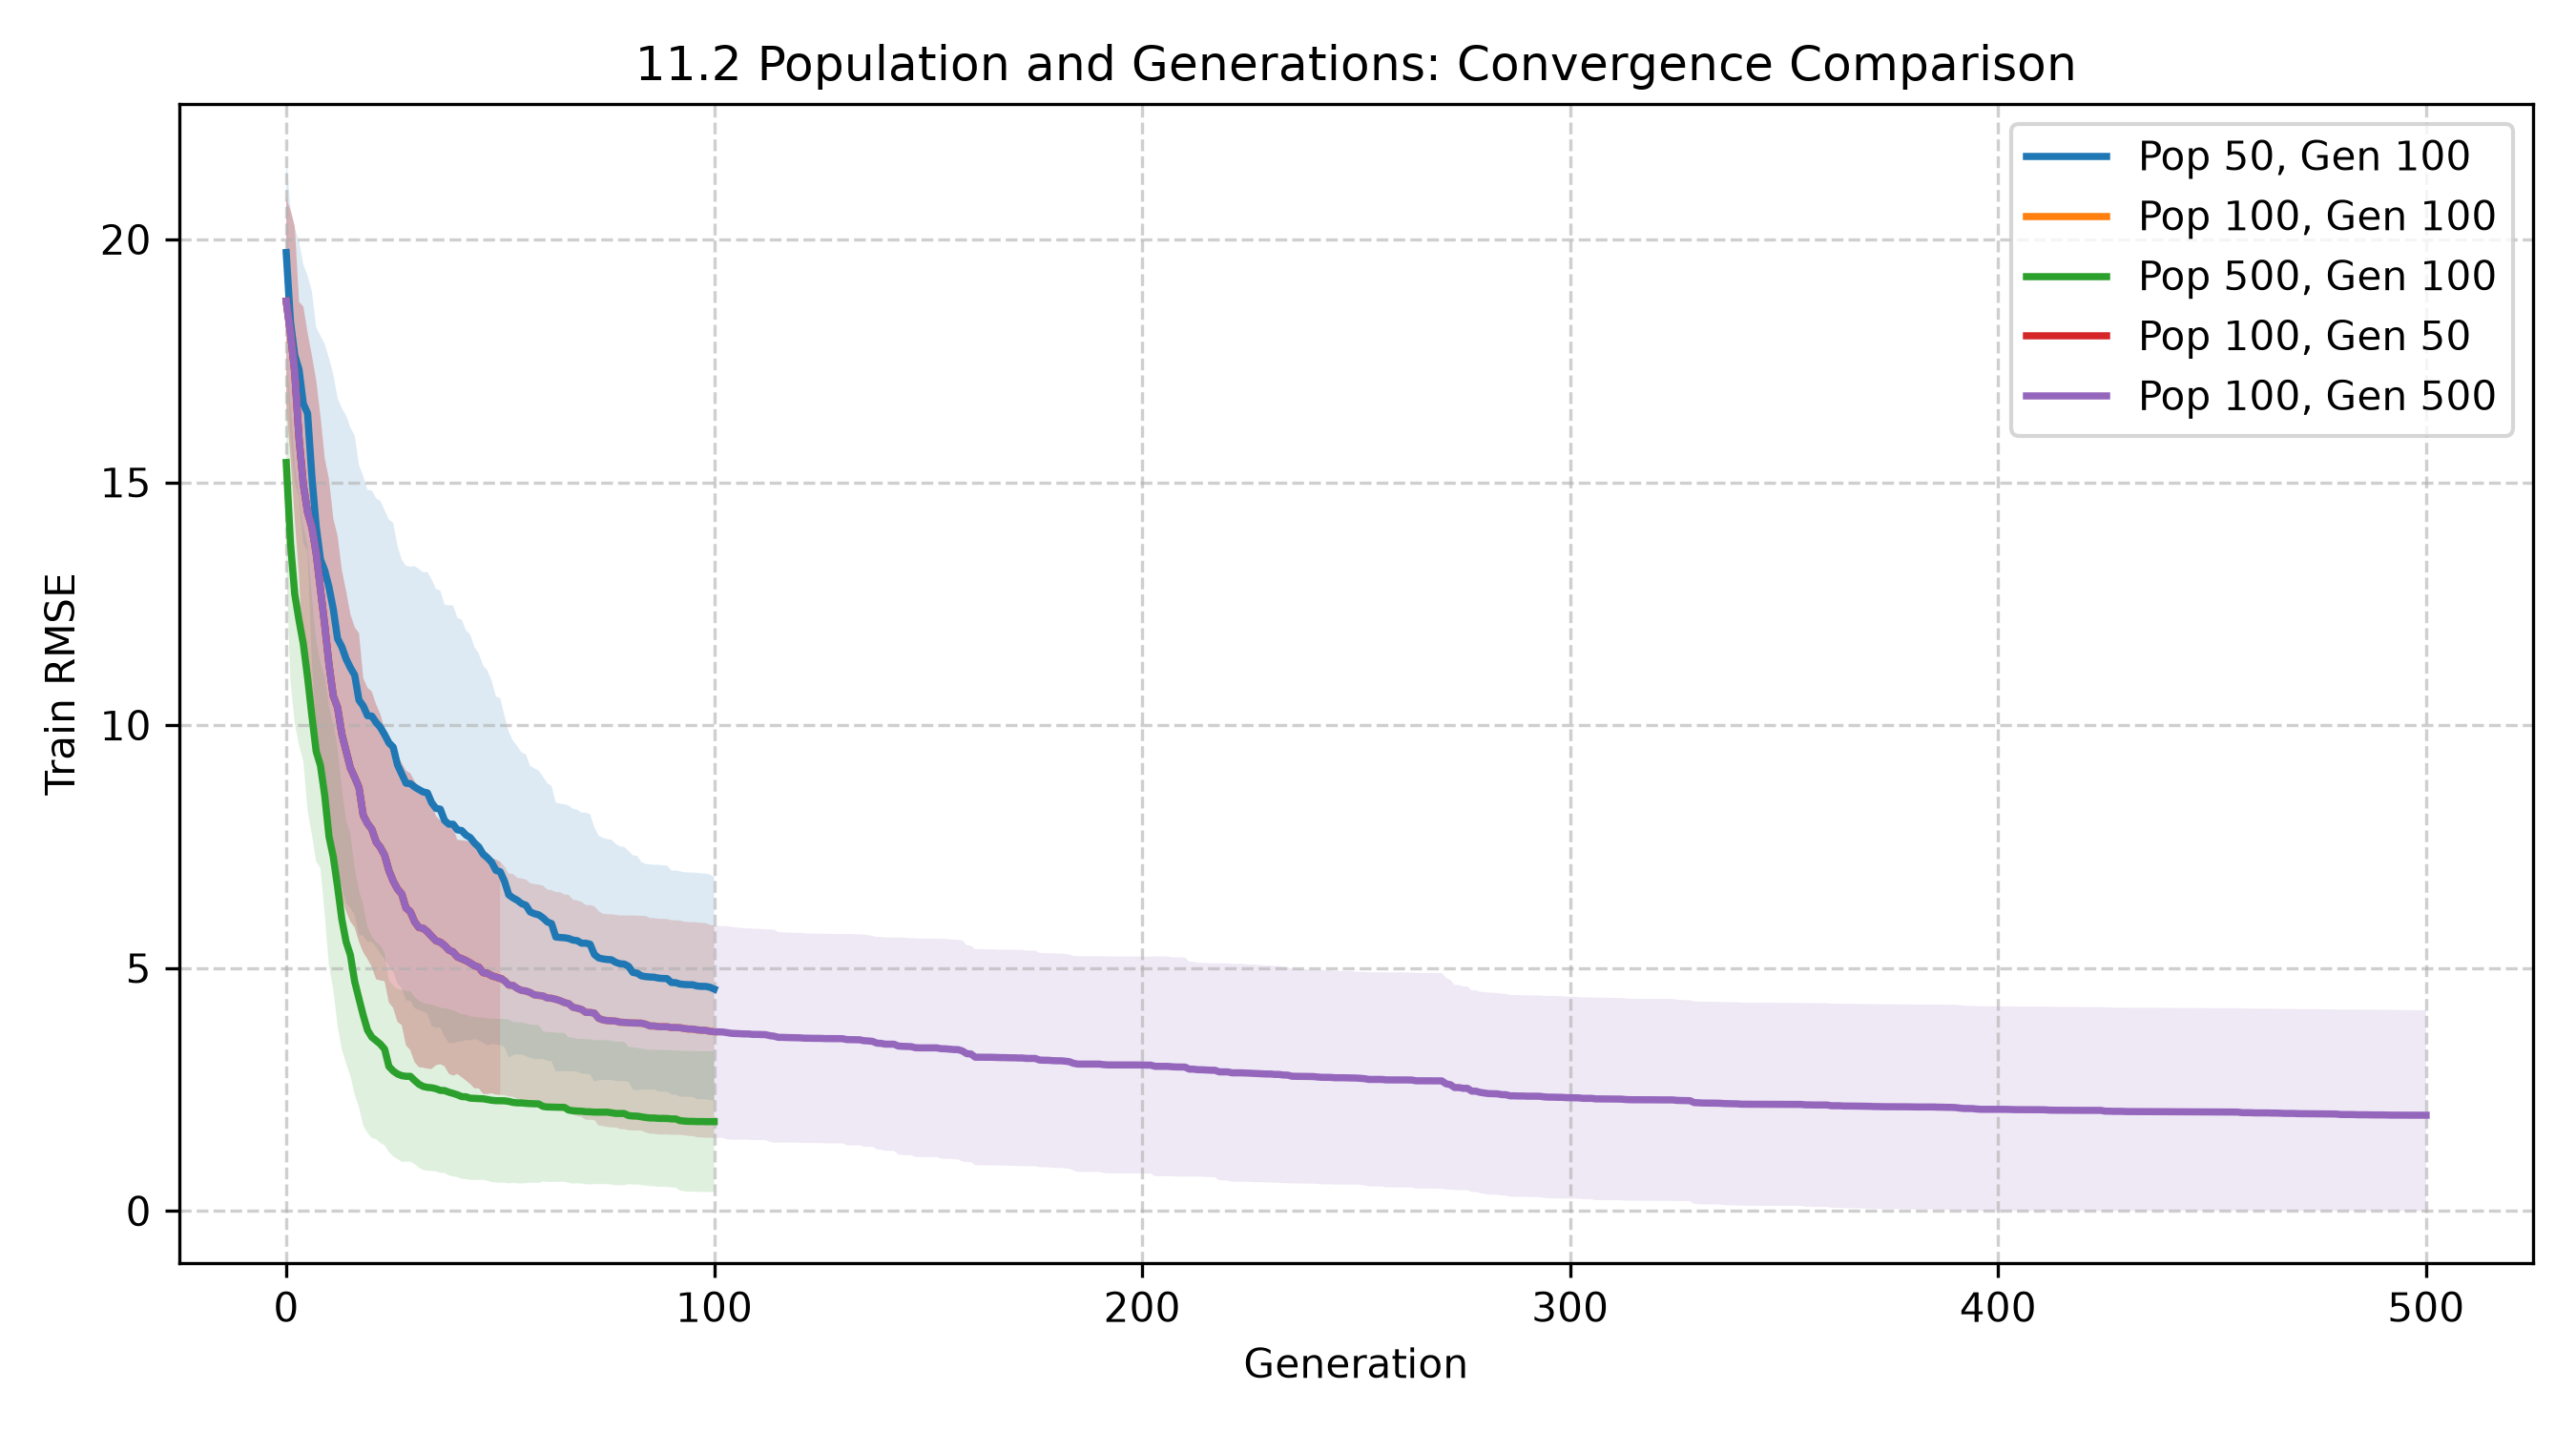
\includegraphics[width=\linewidth]{pop_gens_convergence.png}
    \caption{Convergência (melhor RMSE de treino).}
  \end{subfigure}\hfill
  \begin{subfigure}{0.42\linewidth}
    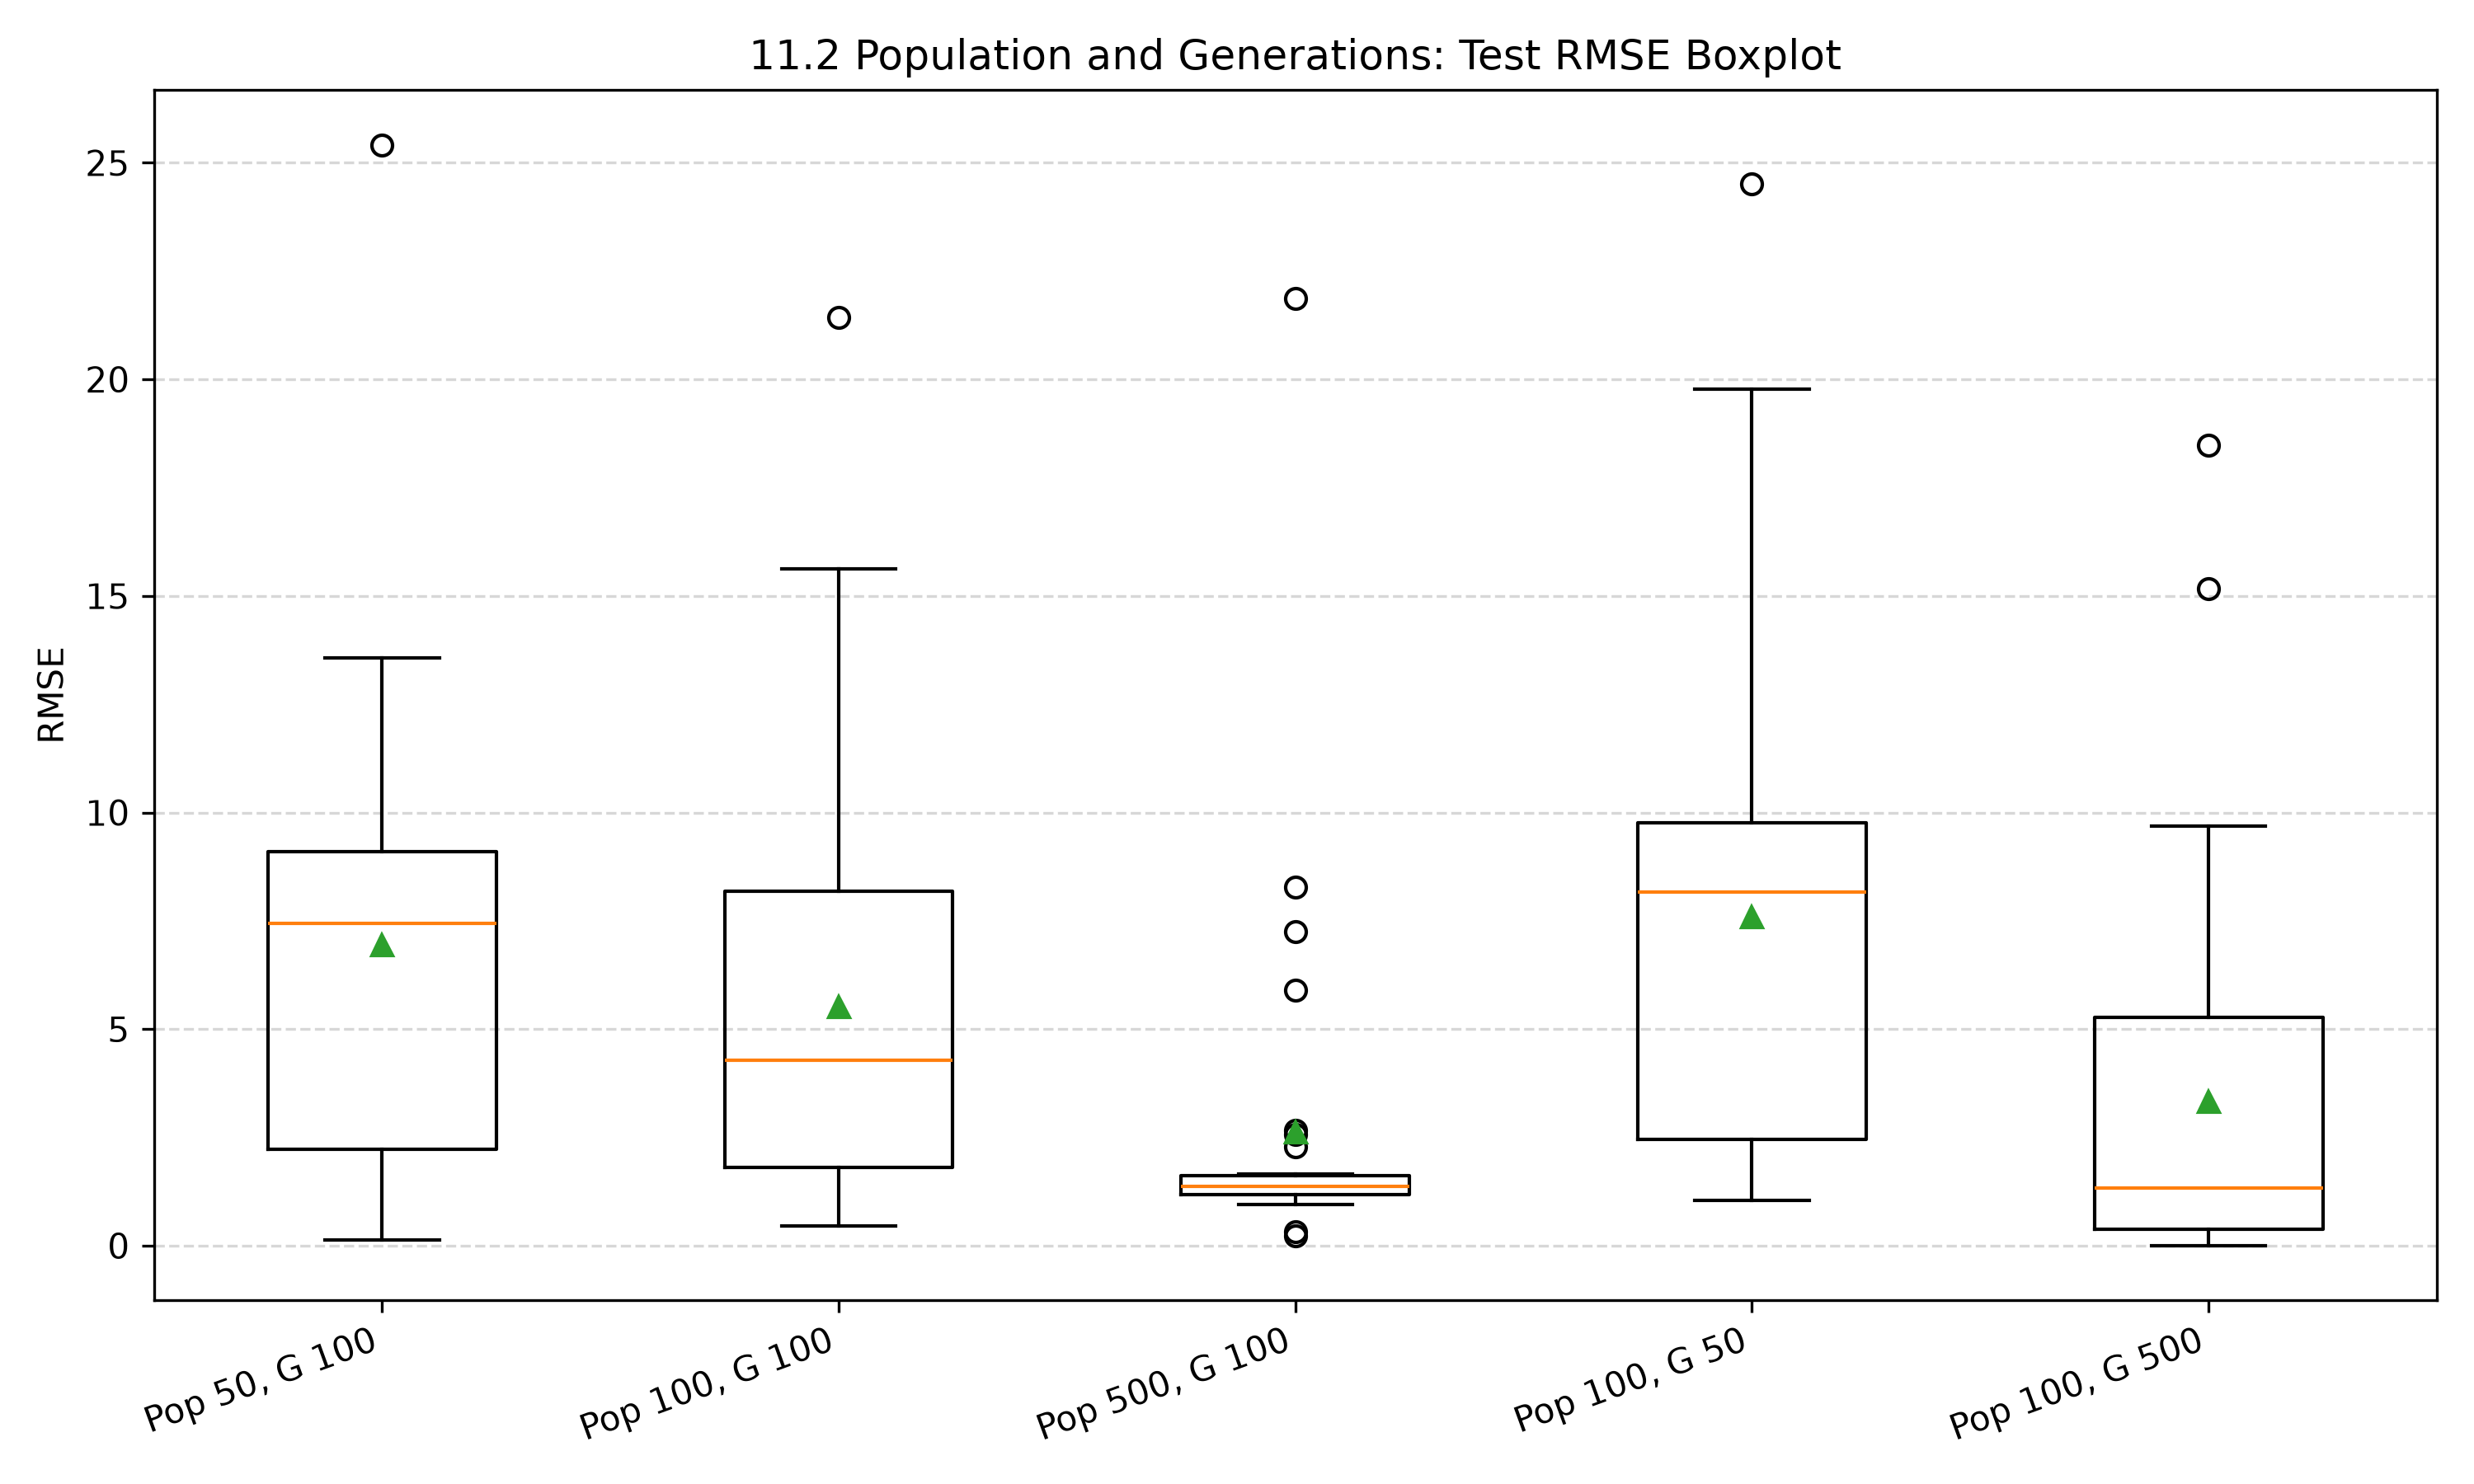
\includegraphics[width=\linewidth]{pop_gens_test_boxplot.png}
    \caption{RMSE de teste.}
  \end{subfigure}
  \caption{Efeito da população e do número de gerações no \code{synth1}.}
  \label{fig:f1_popgen}
\end{figure}

A \cref{tab:f1_popgen} e a \cref{fig:f1_popgen} mostram que aumentar o
orçamento de avaliações reduz o erro: as duas configurações com 50\,000
avaliações são significativamente melhores que a base ($p<0.005$). Já as
configurações com 5\,000 avaliações são piores, embora sem significância a
$5\%$ pelo teste não pareado.

\paragraph{População versus gerações.} Com o mesmo orçamento (50\,000
avaliações), \code{pop=500} e \code{gen=500} não diferem significativamente
na mediana ($p=0.50$), mas \code{pop=500} apresenta IQR dez vezes menor
($0.43$ contra $4.89$), árvores $35\%$ menores ($41.8$ contra $64.2$ nós) e
menor tempo de execução. Prolongar a evolução depois da saturação (por volta
da geração~80) alimenta principalmente o crescimento das árvores, enquanto
ampliar a população aumenta a cobertura do espaço de busca já na geração~0.

\paragraph{A população converge?} Sim. Com 100 gerações, a curva de treino
atinge $95\%$ da melhoria total por volta da geração~80. O número de
indivíduos repetidos atinge um pico na geração~5 (27 de 100 com torneio) e
depois se estabiliza em torno de 9--11, indicando perda parcial de
diversidade.

\paragraph{Escolha.} Foi mantido \code{pop=100}, \code{gen=100}: é a menor
configuração que satura dentro do orçamento, e é cerca de $6\times$ mais
barata que \code{pop=500}, o que viabilizou as mais de 1\,900 execuções do
estudo. Reconhece-se, porém, que \code{pop=500} seria preferível se o custo
não fosse restritivo.

% -----------------------------------------------------------------------------
\subsubsection{Métodos de seleção}
\label{sec:f1_selecao}

\begin{table}[htbp]
  \centering
  \caption{Métodos de seleção no \code{synth1}. ``Rep.'' é o número médio de
           indivíduos repetidos nas gerações 0, 5, 20 e final. Valores de $p$
           (Mann--Whitney) em relação ao torneio com $k=2$.}
  \label{tab:f1_selecao}
  \small
  \resizebox{\linewidth}{!}{%
  \begin{tabular}{@{}lcccccccr@{}}
    \toprule
    Seleção & RMSE treino & RMSE teste & Mediana (IQR) & Mín./Máx. & $p$ & Sat. & Rep. (G0/5/20/F) & Tempo (s) \\
    \midrule
    Roleta          & $3.16 \pm 2.24$ & $5.66 \pm 8.85$  & 2.17 (7.28) & 0.70 / 48.36  & 0.595 & 80 & 10.5/20.3/14.5/9.1 & 7.8 \\
    Torneio $k=2$   & $3.69 \pm 2.19$ & $5.52 \pm 4.89$  & 4.28 (6.38) & 0.46 / 21.44  & ---   & 80 & 10.5/27.1/10.8/9.0 & 7.8 \\
    Torneio $k=3$   & $4.06 \pm 2.20$ & $13.33 \pm 42.80$& 7.01 (6.38) & 0.20 / 239.17 & 0.530 & 63 & 10.5/26.1/14.0/13.9 & 6.6 \\
    \rowcolor{verde}
    $\eps$-Lexicase & $\mathbf{0.99 \pm 1.21}$ & $\mathbf{1.62 \pm 3.36}$ & \textbf{0.68 (1.12)} & 0.01 / 18.19 & $\mathbf{4.1{\times}10^{-6}}$ & 94 & 10.5/\textbf{4.0}/8.7/13.4 & 22.5 \\
    \bottomrule
  \end{tabular}}
\end{table}

\begin{figure}[htbp]
  \centering
  \begin{subfigure}{0.49\linewidth}
    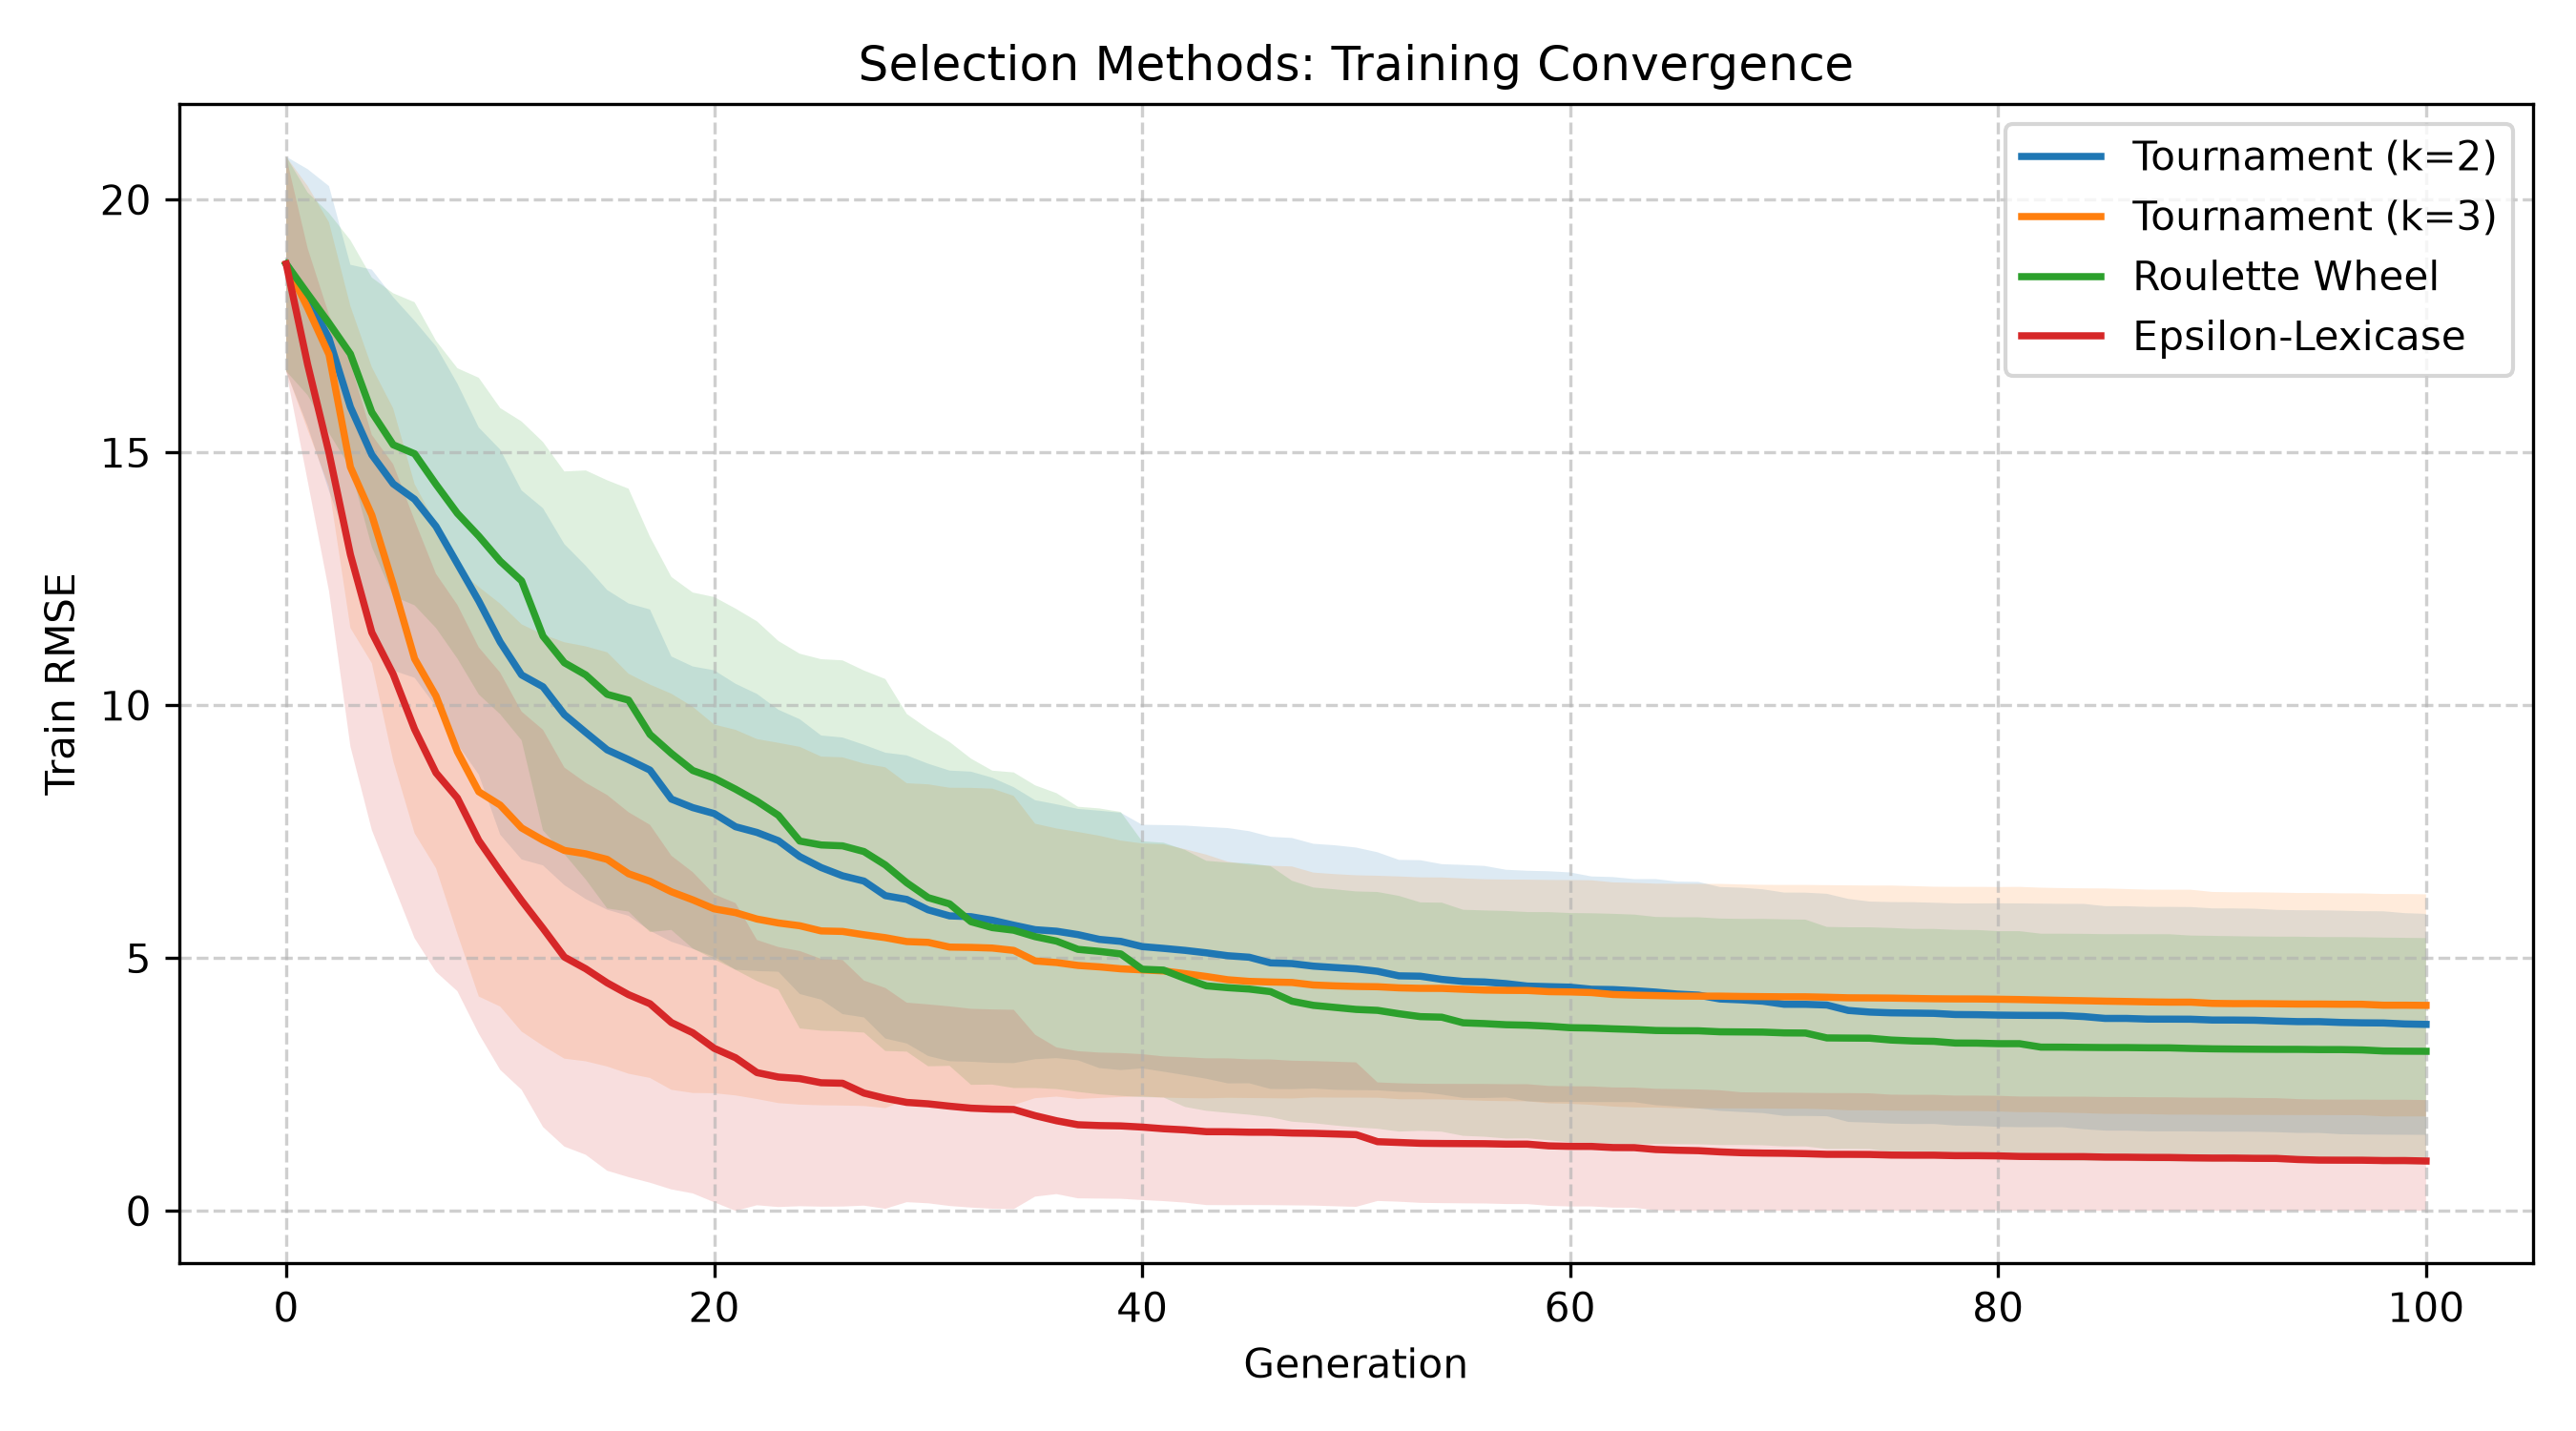
\includegraphics[width=\linewidth]{selection_convergence.png}
    \caption{Convergência.}
  \end{subfigure}\hfill
  \begin{subfigure}{0.49\linewidth}
    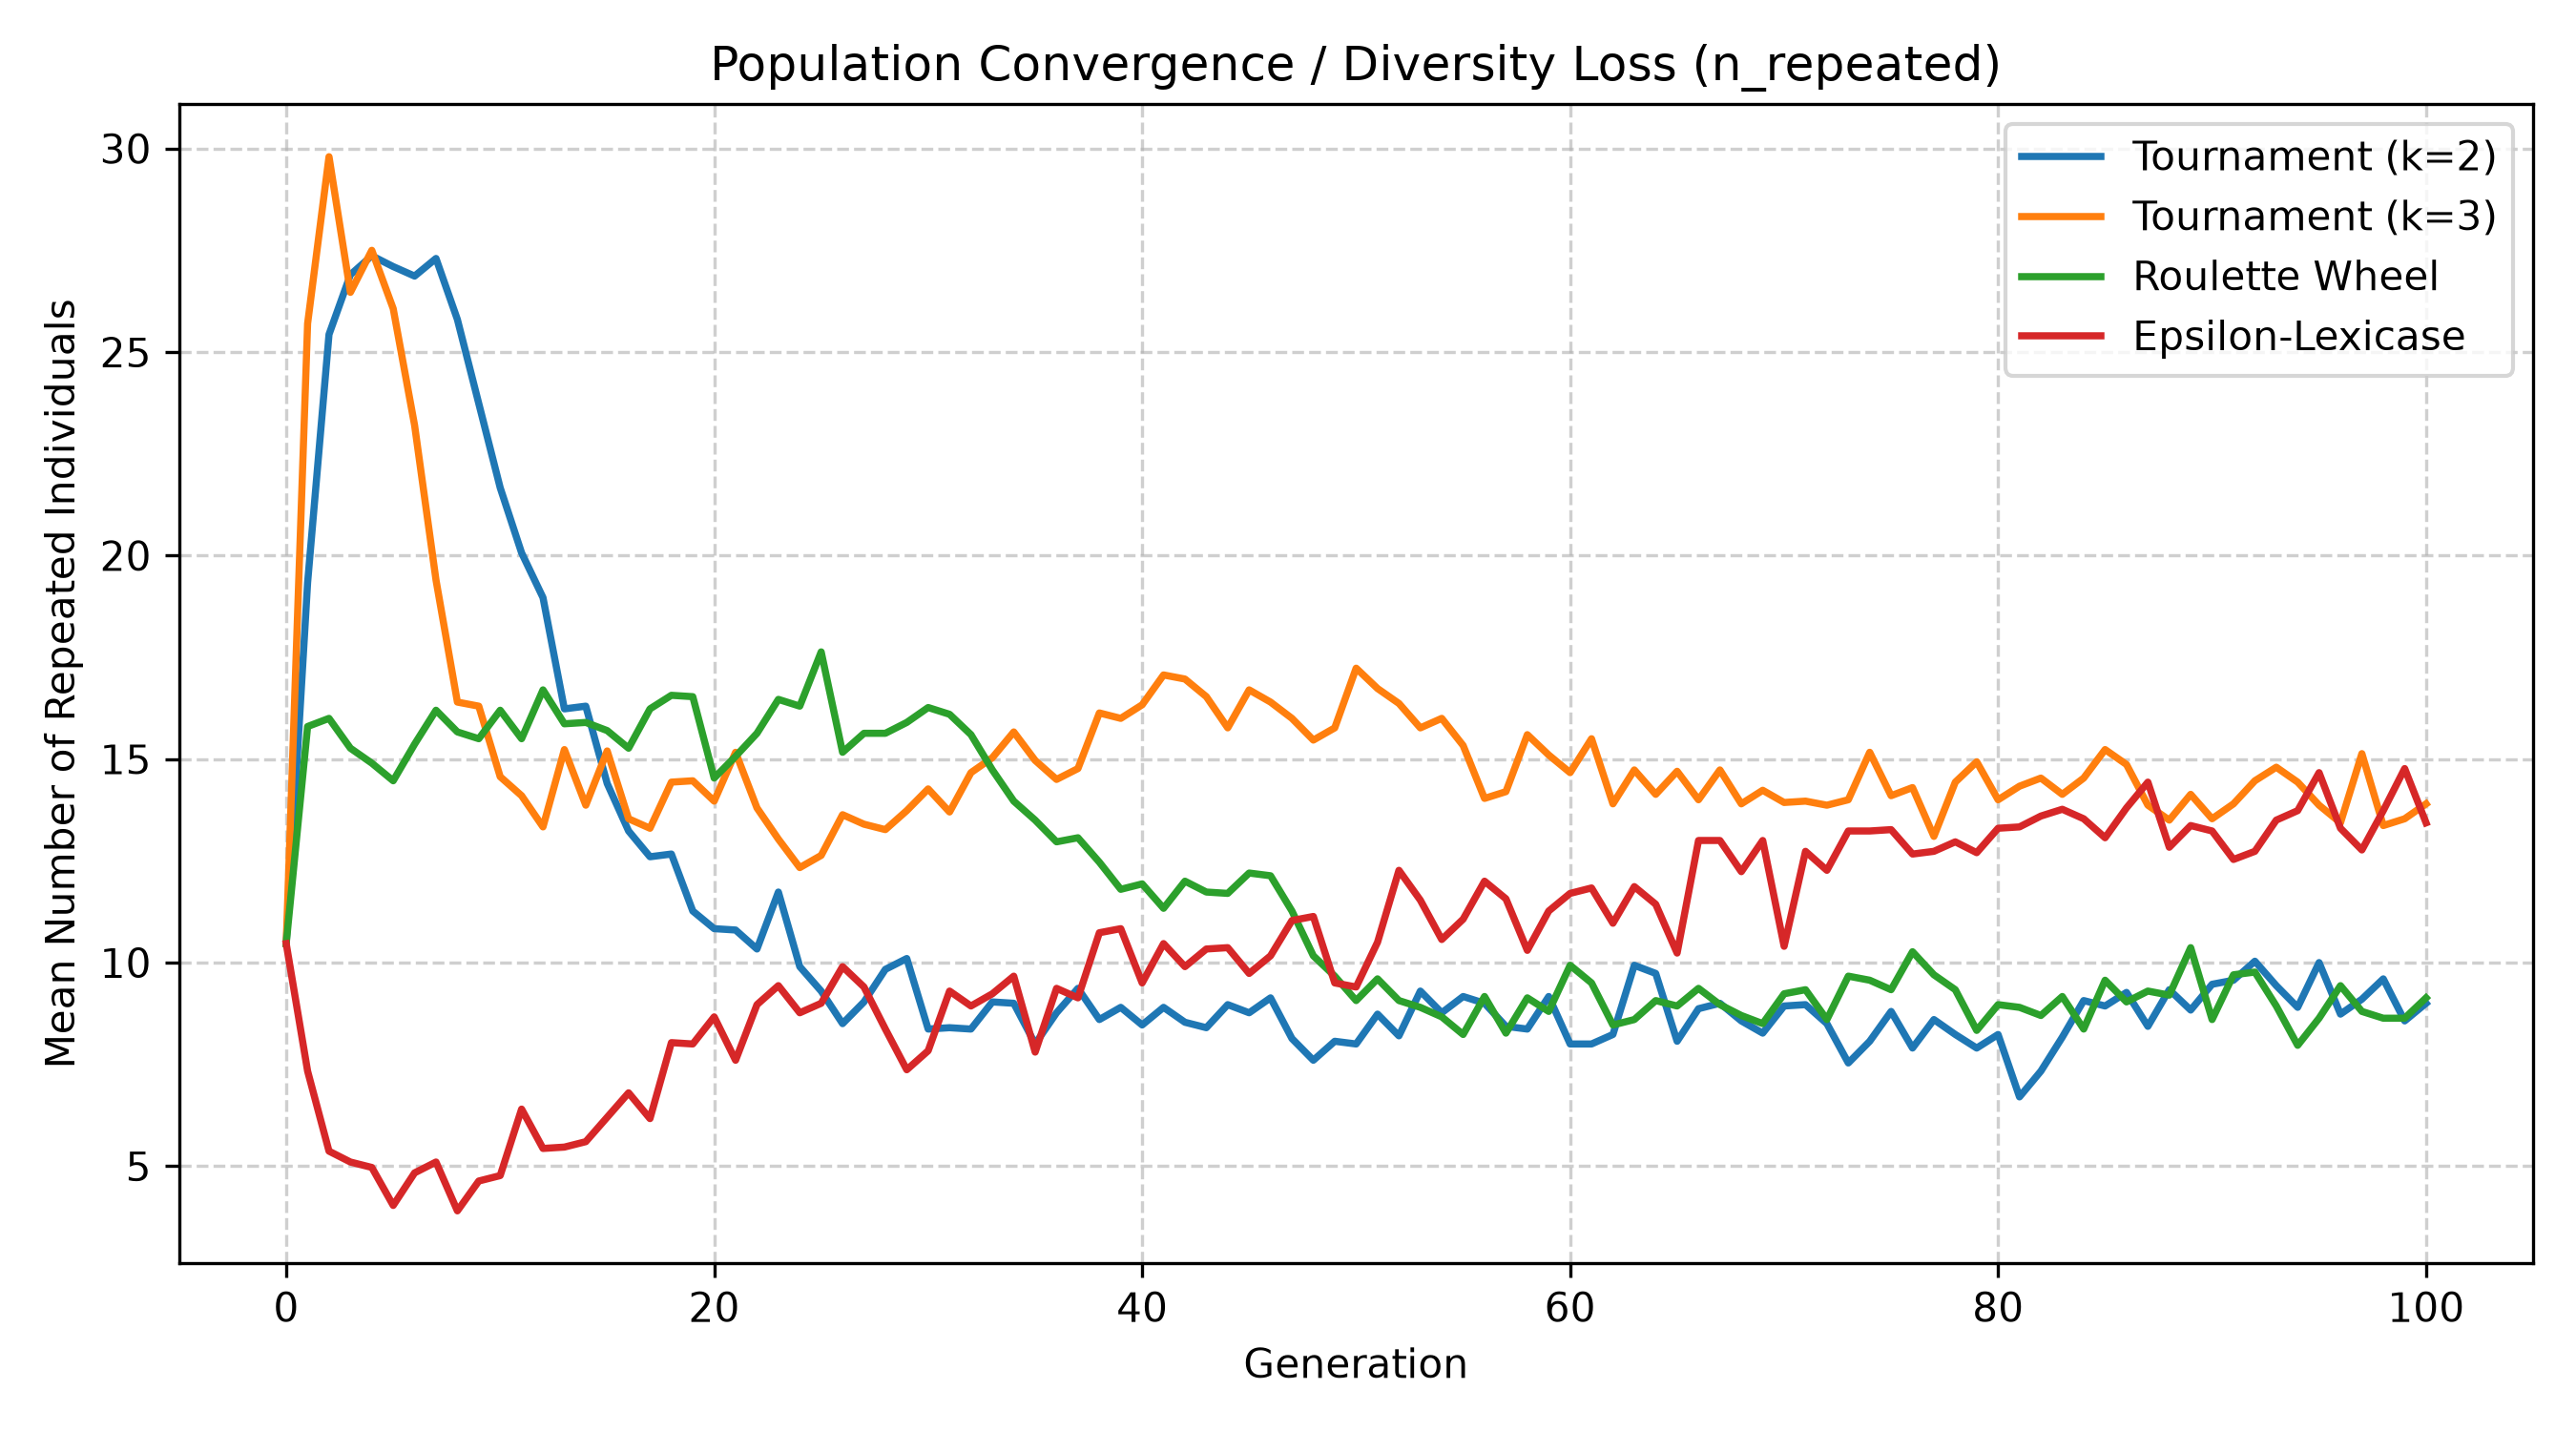
\includegraphics[width=\linewidth]{selection_diversity_n_repeated.png}
    \caption{Indivíduos repetidos por geração.}
  \end{subfigure}
  \caption{Dinâmica dos métodos de seleção no \code{synth1}.}
  \label{fig:f1_selecao}
\end{figure}

A $\eps$-lexicase foi o \textbf{único fator da Fase~1 com efeito
estatisticamente significativo} sobre a configuração base
(\cref{tab:f1_selecao}): o RMSE médio de teste caiu $70.7\%$
($5.52\to1.62$; $p=4.1\times10^{-6}$; 26 vitórias em 30 sementes), e a mediana
caiu de $4.28$ para $0.68$. As mudanças observadas ao trocar a seleção foram:

\begin{itemize}
  \item \textbf{Roleta:} a transformação $1/(1+\mathrm{RMSE})$ achata as
        diferenças entre indivíduos e reduz a pressão seletiva. O resultado
        não difere significativamente do torneio ($p=0.595$), mas a
        variância no teste é muito maior (desvio de $8.85$, máximo de
        $48.4$).
  \item \textbf{Torneio $k=3$:} o aumento da pressão seletiva antecipa a
        saturação (geração~63 contra~80) e produz execuções catastróficas no
        teste (máximo de $239$), um sinal de convergência prematura para
        expressões que extrapolam mal.
  \item \textbf{$\eps$-Lexicase:} na geração~5, o número de clones cai de
        27.1 (torneio) para 4.0, e a população continua melhorando até a
        geração~94 (\cref{fig:f1_selecao}). Ao selecionar especialistas em
        subconjuntos distintos de casos, o método mantém múltiplas
        linhagens e evita que um único indivíduo domine a população cedo.
        O custo é cerca de $3\times$ maior, devido à filtragem caso a caso.
\end{itemize}

% -----------------------------------------------------------------------------
\subsubsection{\emph{Crossover} e mutação}
\label{sec:f1_operadores}

Conforme estabelecido no guia experimental do enunciado, foram investigadas duas
configurações de partida para os operadores genéticos de variação:
(i)~\textbf{Configuração~A} ($\pc=0.90$, $\pmut=0.05$), que adota o regime
canônico clássico de Koza onde o \emph{crossover} atua como o principal motor
evolutivo e a mutação é mantida em nível residual; e
(ii)~\textbf{Configuração~B} ($\pc=0.60$, $\pmut=0.30$), que testa uma hipótese
balanceada com mutação substancialmente mais agressiva ($6\times$ superior) e
cruzamento atenuado, investigando se uma exploração local mais frequente previne
a estagnação prematura. Subsequentemente, realizaram-se varreduras
unidimensionais de $\pc\in\{0.5,0.7,0.9\}$ e $\pmut\in\{0.01,0.05,0.1,0.2\}$,
todas fixando seleção por torneio $k=2$ (\cref{tab:f1_operadores}).

\begin{table}[htbp]
  \centering
  \caption{Contribuição dos operadores no \code{synth1} (totais médios por
           execução em 100 gerações). ``Cx $>$ média'' e ``Cx $>$ melhor''
           indicam a fração de filhos de \emph{crossover} melhores que a
           média dos pais e que o melhor pai, respectivamente.}
  \label{tab:f1_operadores}
  \small
  \resizebox{\linewidth}{!}{%
  \begin{tabular}{@{}lccccccc@{}}
    \toprule
    Config. & Cx melhor/pior (média pais) & Cx $>$ média & Cx $>$ melhor & Mut. $+$ (bruta)$^a$ & Mut. $+$ (corrigida)$^b$ & RMSE teste & Mediana (IQR) \\
    \midrule
    A: $\pc{=}0.9$, $\pmut{=}0.05$ & 2643.6 / 5606.1 & 32.0\% & 11.0\% & 92.5\% & $\approx$25\% & $5.52 \pm 4.89$ & 4.28 (6.38) \\
    B: $\pc{=}0.6$, $\pmut{=}0.30$ & 1233.5 / 2894.4 & 29.9\% & 11.5\% & 69.3\% & $\approx$23\% & $5.96 \pm 4.52$ & 7.79 (7.98) \\
    \midrule
    $\pc{=}0.5$, $\pmut{=}0.05$    &  955.6 / 3516.4 & 21.4\% &  5.4\% & 56.4\% & $\approx$13\% & $7.92 \pm 9.12$ & 7.48 (7.16) \\
    \rowcolor{verde}
    $\pc{=}0.7$, $\pmut{=}0.05$    & 1744.5 / 4627.2 & 27.4\% &  8.5\% & 75.9\% & $\approx$20\% & $3.97 \pm 3.41$ & 2.09 (6.54) \\
    $\pc{=}0.9$, $\pmut{=}0.01$    & 2709.6 / 5886.8 & 31.5\% & 10.5\% & 92.5\% & $\approx$25\% & $6.46 \pm 4.27$ & 7.26 (6.26) \\
    \rowcolor{verde}
    $\pc{=}0.9$, $\pmut{=}0.10$    & 2575.9 / 5332.8 & 32.6\% & 12.3\% & 92.2\% & $\approx$22\% & $3.89 \pm 3.15$ & 2.47 (5.93) \\
    $\pc{=}0.9$, $\pmut{=}0.20$    & 2390.5 / 4693.7 & 33.7\% & 13.9\% & 92.8\% & $\approx$28\% & $6.53 \pm 4.16$ & 8.03 (6.70) \\
    \bottomrule
  \end{tabular}}

  \vspace{3pt}
  \raggedright\footnotesize
  $^a$ Fração de mutações que melhoraram a aptidão, conforme registrada pelo arcabouço.\\
  $^b$ Estimativa que remove o artefato descrito no texto: $(b-\pc N)/((1-\pc)N)$, com $b$ o número de mutações benéficas e $N$ o total de mutações não neutras.
\end{table}

\begin{figure}[htbp]
  \centering
  \begin{subfigure}{0.49\linewidth}
    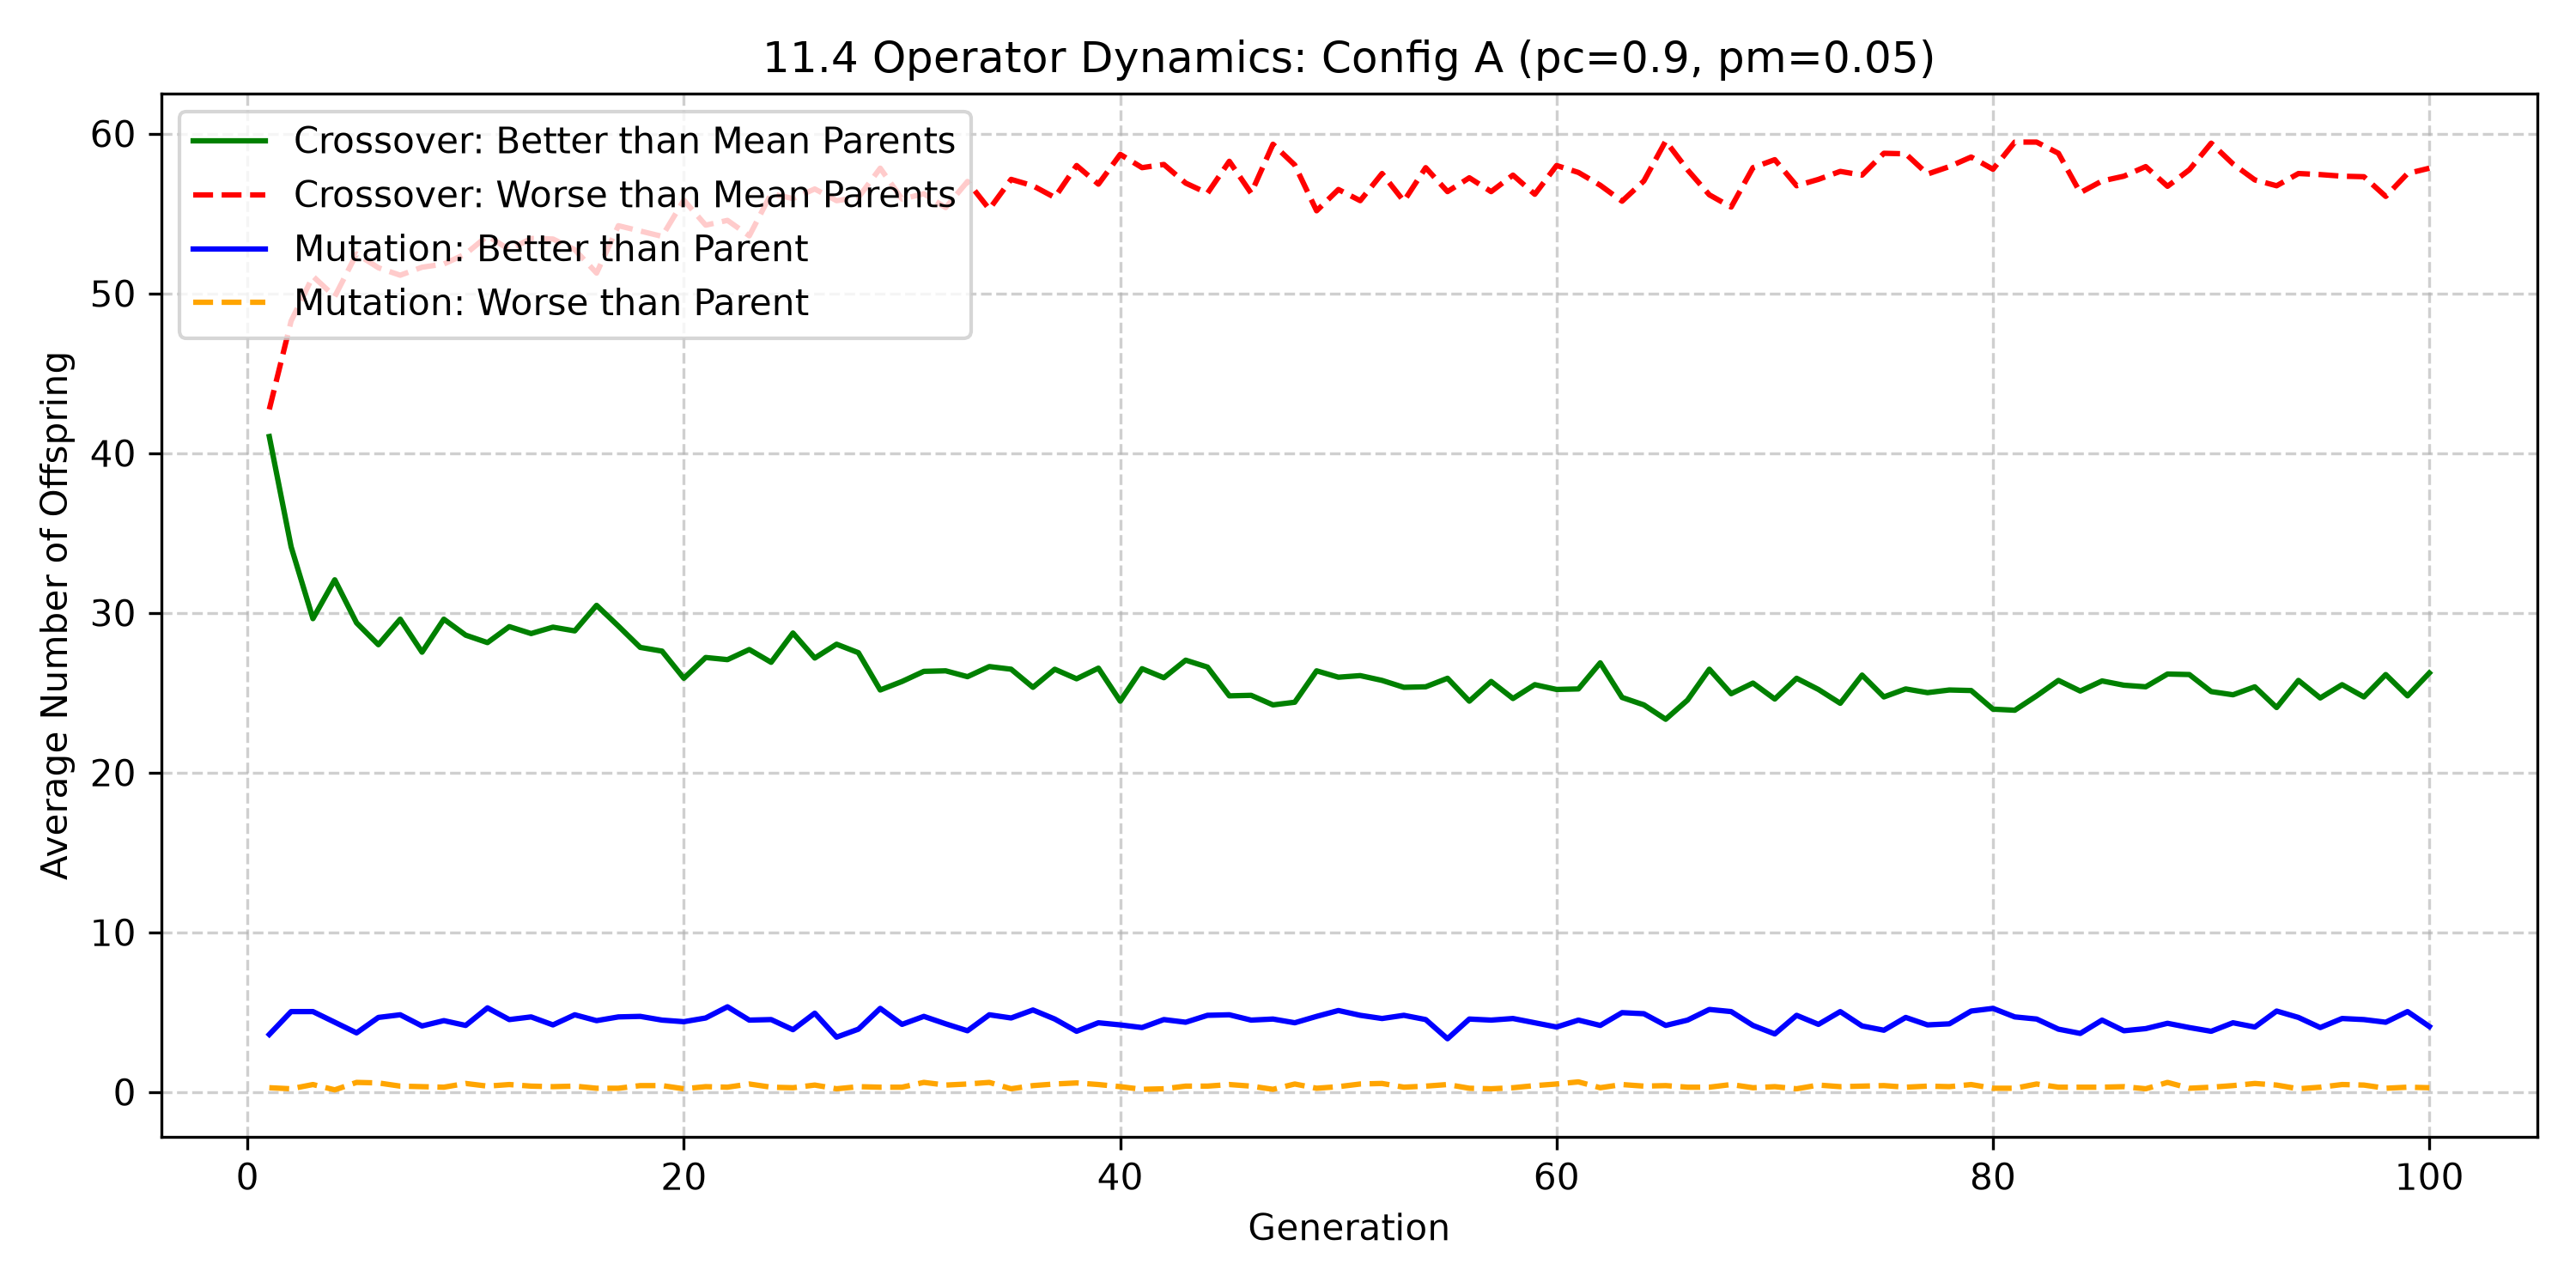
\includegraphics[width=\linewidth]{operator_dynamics_config_A.png}
    \caption{Config.~A ($\pc=0.9$, $\pmut=0.05$).}
  \end{subfigure}\hfill
  \begin{subfigure}{0.49\linewidth}
    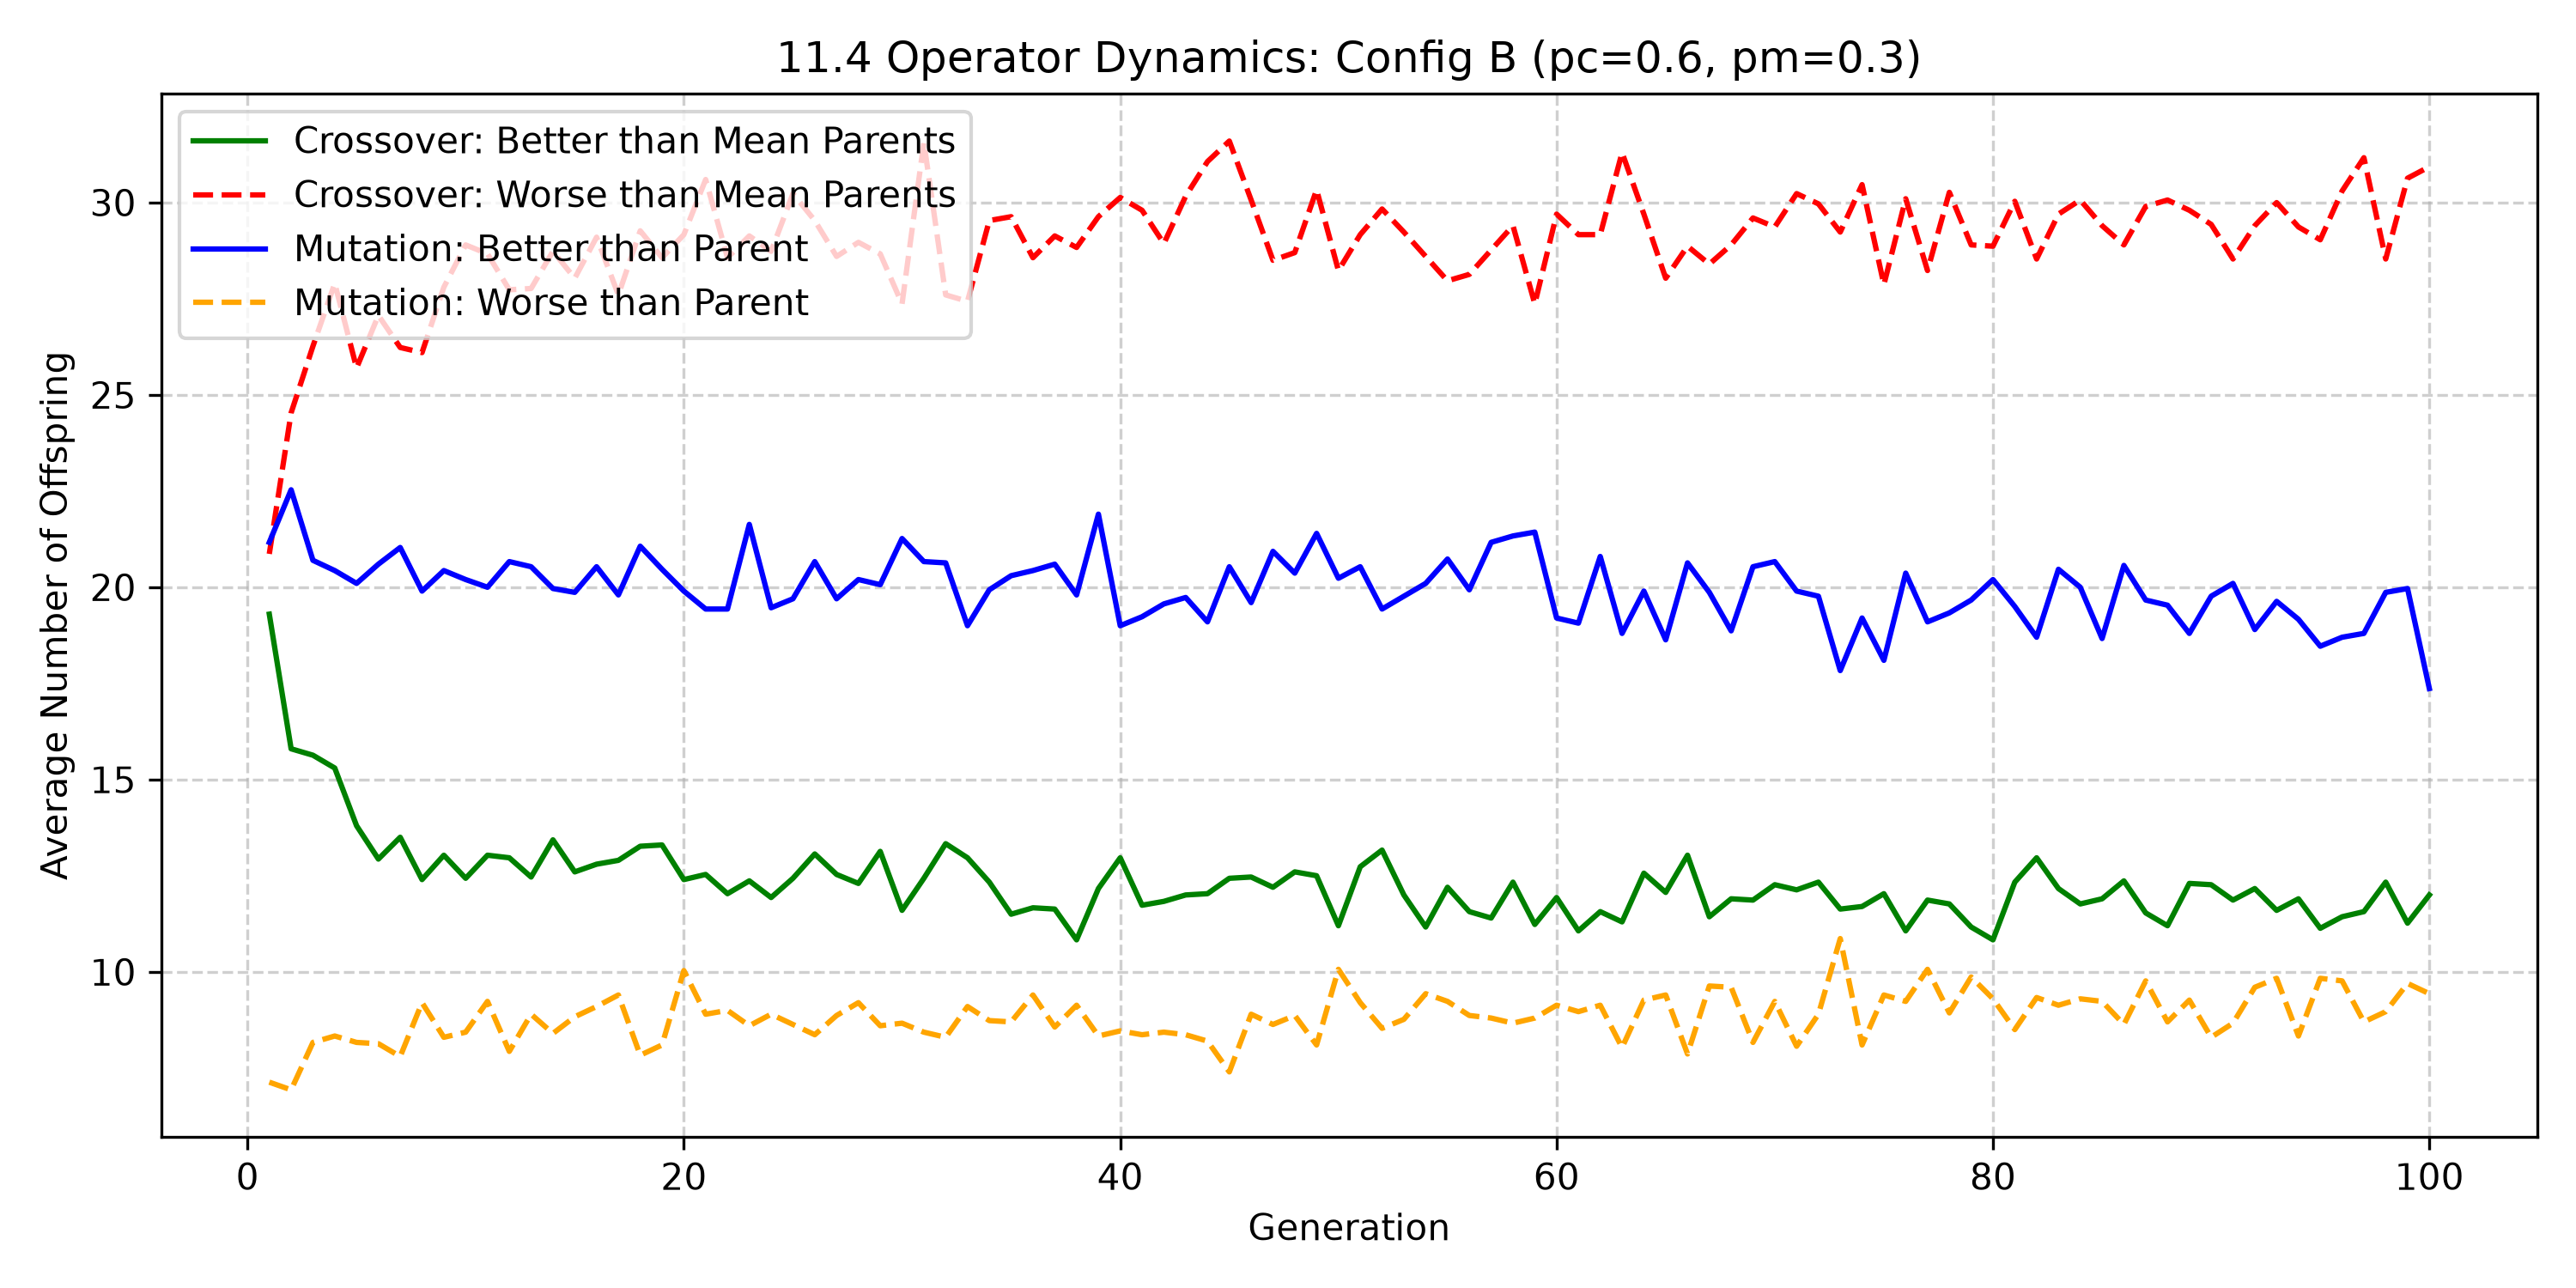
\includegraphics[width=\linewidth]{operator_dynamics_config_B.png}
    \caption{Config.~B ($\pc=0.6$, $\pmut=0.3$).}
  \end{subfigure}
  \caption{Número de filhos melhores e piores que os pais por geração.}
  \label{fig:f1_operadores}
\end{figure}

\paragraph{Em quantos casos cada operador contribui?} O \emph{crossover} é
predominantemente destrutivo: na Config.~A, apenas $32\%$ dos filhos superam
a média dos pais e apenas $11\%$ superam o melhor pai, ou seja, $89\%$ das
recombinações pioram o melhor material genético disponível. A
\cref{fig:f1_operadores} mostra que a fração positiva é máxima nas primeiras
gerações (cerca de 41 filhos melhores que a média dos pais na geração~1) e
cai rapidamente para cerca de 25 por geração, à medida que a população se
especializa e a troca de subárvores passa a desmontar expressões já
ajustadas. A produtividade em relação ao melhor pai cai de $10.1$ filhos por
geração (gerações 1--20) para $6.8$ (gerações 81--100).

\paragraph{Artefato na métrica de mutação.} A taxa de sucesso bruta da
mutação ($\approx92\%$ com $\pc=0.9$) está \textbf{superestimada}. Quando a
mutação é aplicada a um filho recém-gerado por \emph{crossover}, esse filho
ainda não foi avaliado, e a sua aptidão ``anterior'' é registrada como
$+\infty$. Assim, toda mutação pós-\emph{crossover} é contada como benéfica.
O indício é que a taxa bruta acompanha $\pc$ (56\%, 69\%, 76\% e 92\% para
$\pc=0.5$, $0.6$, $0.7$ e $0.9$). Removendo a fração esperada de casos
contaminados, a taxa real de mutações benéficas fica entre $13\%$ e $28\%$
(\cref{tab:f1_operadores}). Ou seja, a mutação de subárvore também é
majoritariamente destrutiva, embora menos que o \emph{crossover} em relação
ao melhor pai. O artefato não afeta a evolução, apenas a estatística.

\paragraph{Config.~A versus Config.~B.} Não há diferença significativa
($p=0.641$). A Config.~B produz árvores menores ($37.5$ contra $46.5$ nós),
mas a mutação de subárvore a $30\%$ substitui blocos inteiros de soluções
boas, e a mediana sobe de $4.28$ para $7.79$.

\paragraph{Valores propostos.} As varreduras indicam um ótimo
\emph{intermediário}: tanto reduzir $\pc$ para $0.7$ (mediana $2.09$) quanto
elevar $\pmut$ para $0.1$ (mediana $2.47$) melhoram a configuração base, e os
extremos ($\pc=0.5$, $\pmut=0.01$ ou $\pmut=0.2$) pioram. Nenhuma dessas
diferenças é significativa isoladamente ($p>0.3$), por causa da
bimodalidade. A proposta resultante, $\pc\approx0.7$ e
$\pmut\in[0.1,0.15]$, \textbf{não foi testada em conjunto na Fase~1}, mas ela foi
validada na Fase~2 (hipótese H2). Os parâmetros anteriores (população e
gerações) permanecem adequados: em todas as varreduras, a saturação ocorre
antes da geração~100.

% -----------------------------------------------------------------------------
\subsubsection{Elitismo}
\label{sec:f1_elitismo}

\begin{table}[htbp]
  \centering
  \caption{Efeito do elitismo no \code{synth1} (torneio $k=2$).}
  \label{tab:f1_elitismo}
  \small
  \begin{tabular}{@{}lccccc@{}}
    \toprule
    Configuração & RMSE treino & RMSE teste & Mediana (IQR) & Mín./Máx. & Tam. melhor \\
    \midrule
    \rowcolor{verde}
    Com elitismo (1) & $3.69 \pm 2.19$ & $5.52 \pm 4.89$ & 4.28 (6.38) & 0.46 / 21.44 & $46.5 \pm 17.5$ \\
    Sem elitismo     & $4.91 \pm 1.91$ & $6.57 \pm 3.07$ & 8.16 (2.90) & 0.94 / 10.97 & $54.3 \pm 15.6$ \\
    \bottomrule
  \end{tabular}
\end{table}

\begin{figure}[htbp]
  \centering
  \begin{subfigure}{0.56\linewidth}
    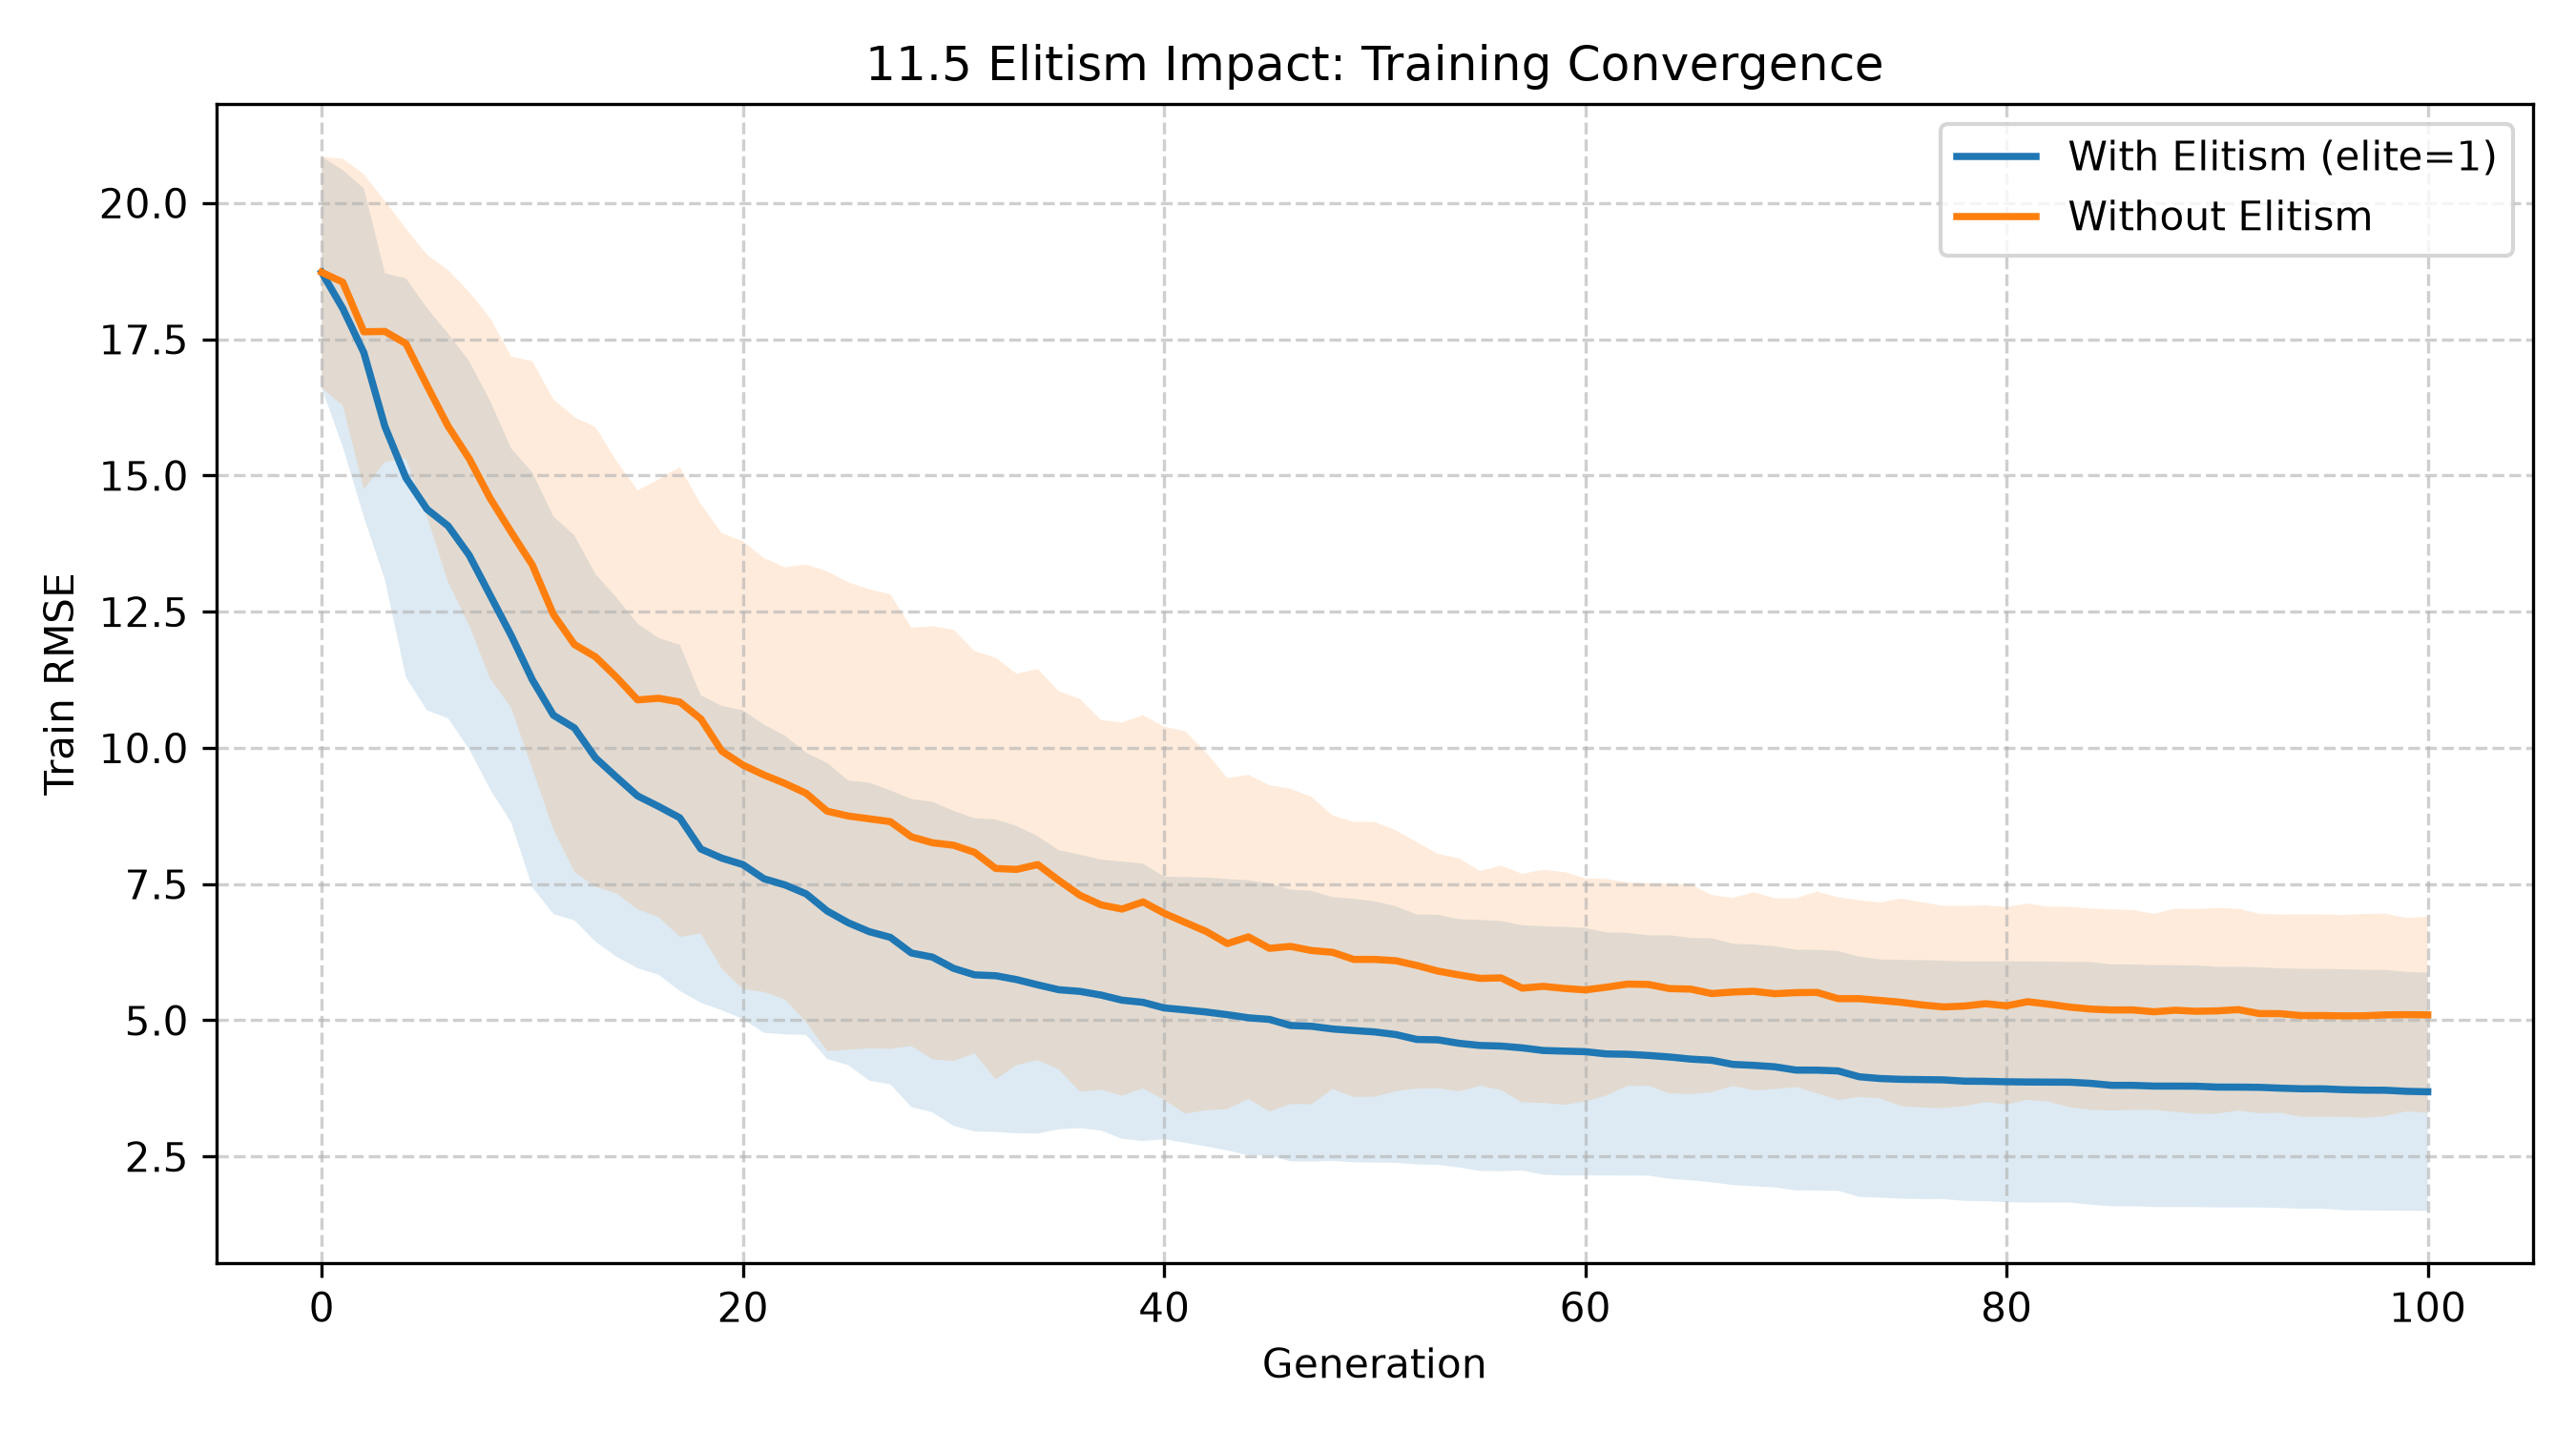
\includegraphics[width=\linewidth]{elitism_convergence.png}
  \end{subfigure}\hfill
  \begin{subfigure}{0.42\linewidth}
    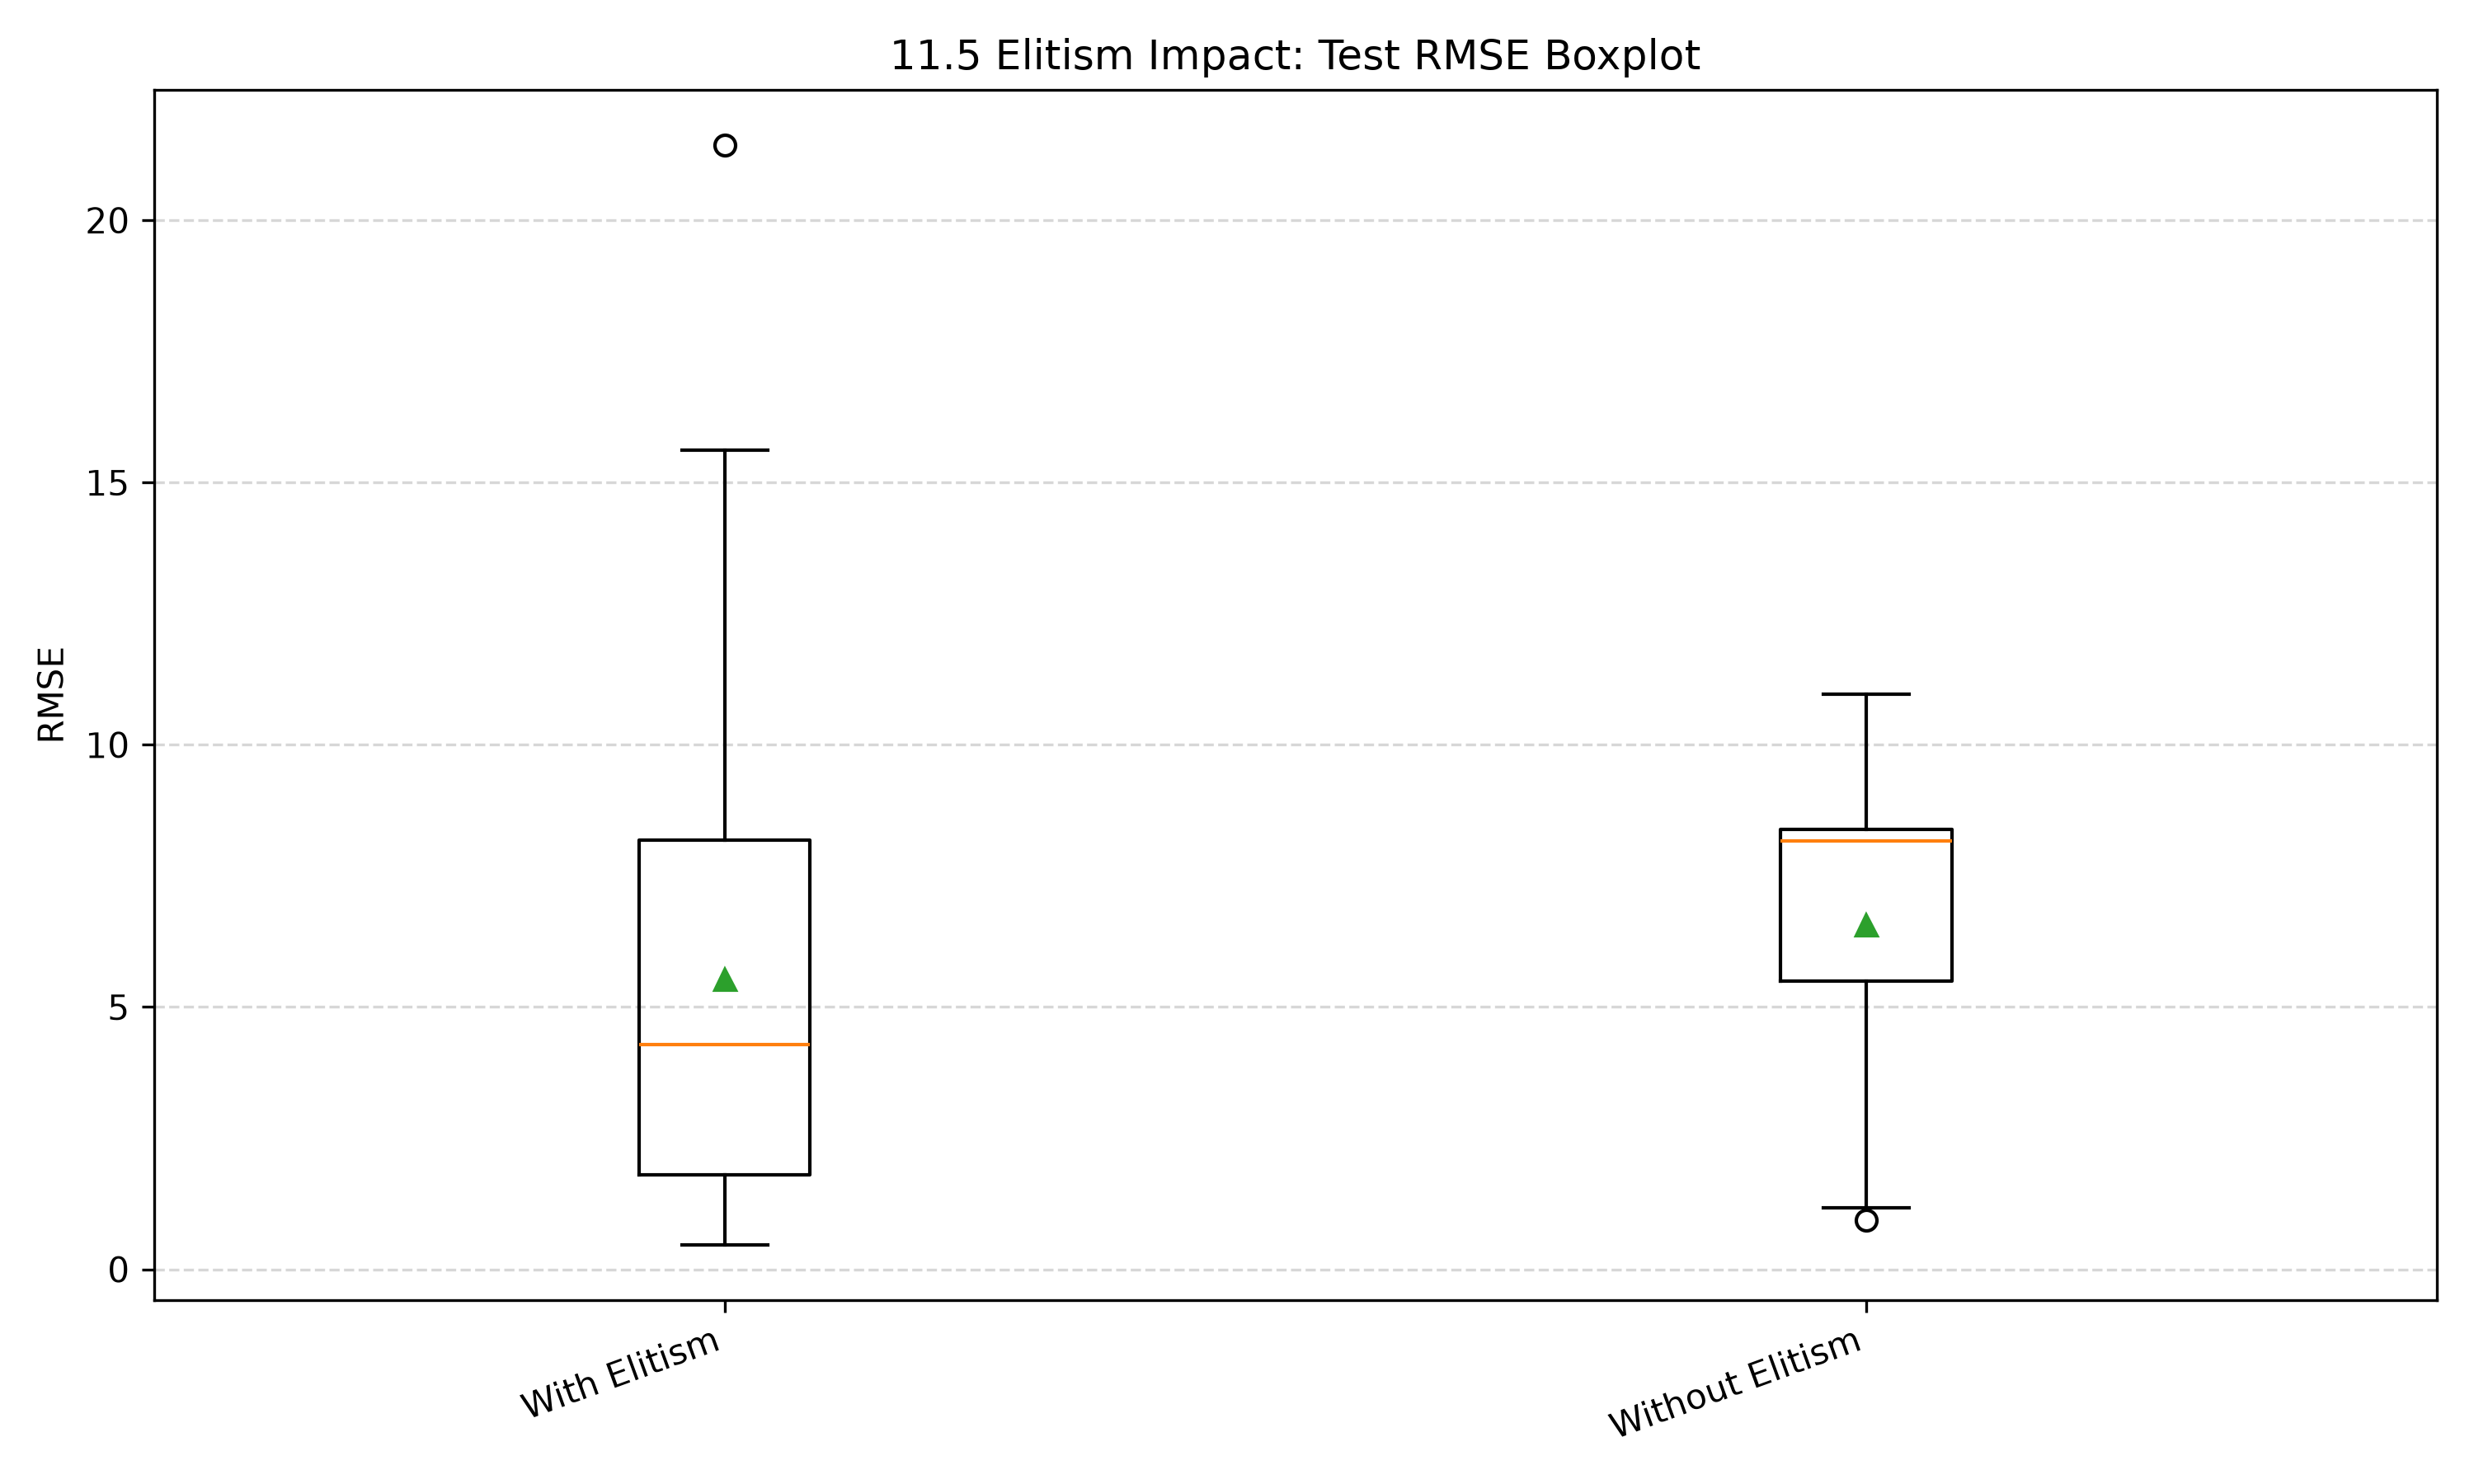
\includegraphics[width=\linewidth]{elitism_test_boxplot.png}
  \end{subfigure}
  \caption{Convergência e RMSE de teste com e sem elitismo.}
  \label{fig:f1_elitismo}
\end{figure}

Sem elitismo, o RMSE de treino piora $33\%$ e a mediana de teste quase dobra
($4.28\to8.16$), como mostram a \cref{tab:f1_elitismo} e a
\cref{fig:f1_elitismo}. Como cerca de $89\%$ dos cruzamentos pioram o melhor
pai, a melhor solução é frequentemente destruída, e a curva do melhor
indivíduo deixa de ser monotônica. As árvores também crescem
($46.5\to54.3$ nós), o que é compatível com a hipótese de \emph{bloat}
defensivo: árvores maiores, com mais \emph{introns}, sobrevivem melhor a
operadores destrutivos~\cite{langdon1997fitness}. O teste de Mann--Whitney
não acusa diferença significativa ($p=0.158$), pois a ausência de elitismo
também reduz a cauda superior (máximo de $10.97$).

% -----------------------------------------------------------------------------
\subsubsection{\emph{Bloating}}
\label{sec:f1_bloat}

\paragraph{Forma simples de medir.} Uma forma otimizada para identificar a presenta de bloat,
que foi escolhida é, registrar a cada geração
o tamanho médio da população (em nós), o tamanho do melhor indivíduo e a
profundidade média, e confrontá-los com a variação do melhor erro. Há
\emph{bloat} quando o tamanho cresce enquanto o erro estagna, isto é,
$\frac{d\,\overline{\text{tam}}}{dt}>0$ com
$\frac{d\,\text{RMSE}^{*}}{dt}\approx0$. Um indicador escalar útil é o fator
de inchaço $\overline{\text{tam}}_{\text{final}}/\overline{\text{tam}}_{G0}$.

\begin{table}[htbp]
  \centering
  \caption{Indicadores de \emph{bloating} na Fase~1.}
  \label{tab:f1_bloat}
  \small
  \begin{tabular}{@{}lccccc@{}}
    \toprule
    Configuração & Tam. médio (G0 $\to$ final) & Fator & Tam. melhor & RMSE teste & Mediana \\
    \midrule
    \code{synth1}, prof.~7, 100 ger.  & $26.2 \to 50.5$  & $1.93\times$ & $46.5 \pm 17.5$ & $5.52 \pm 4.89$ & 4.28 \\
    \code{synth1}, prof.~10, 100 ger. & $130.7 \to 70.2$ & ---          & $64.4 \pm 25.2$ & $4.82 \pm 4.23$ & 2.38 \\
    \code{synth1}, prof.~7, 500 ger.  & $26.2 \to 66.4$  & $2.53\times$ & $64.2 \pm 21.7$ & $3.33 \pm 4.74$ & 1.33 \\
    \code{concrete1}, prof.~7         & $26.2 \to 72.3$  & $2.76\times$ & $74.1 \pm 27.2$ & $11.97 \pm 1.51$ & 11.65 \\
    \bottomrule
  \end{tabular}
\end{table}

\begin{figure}[htbp]
  \centering
  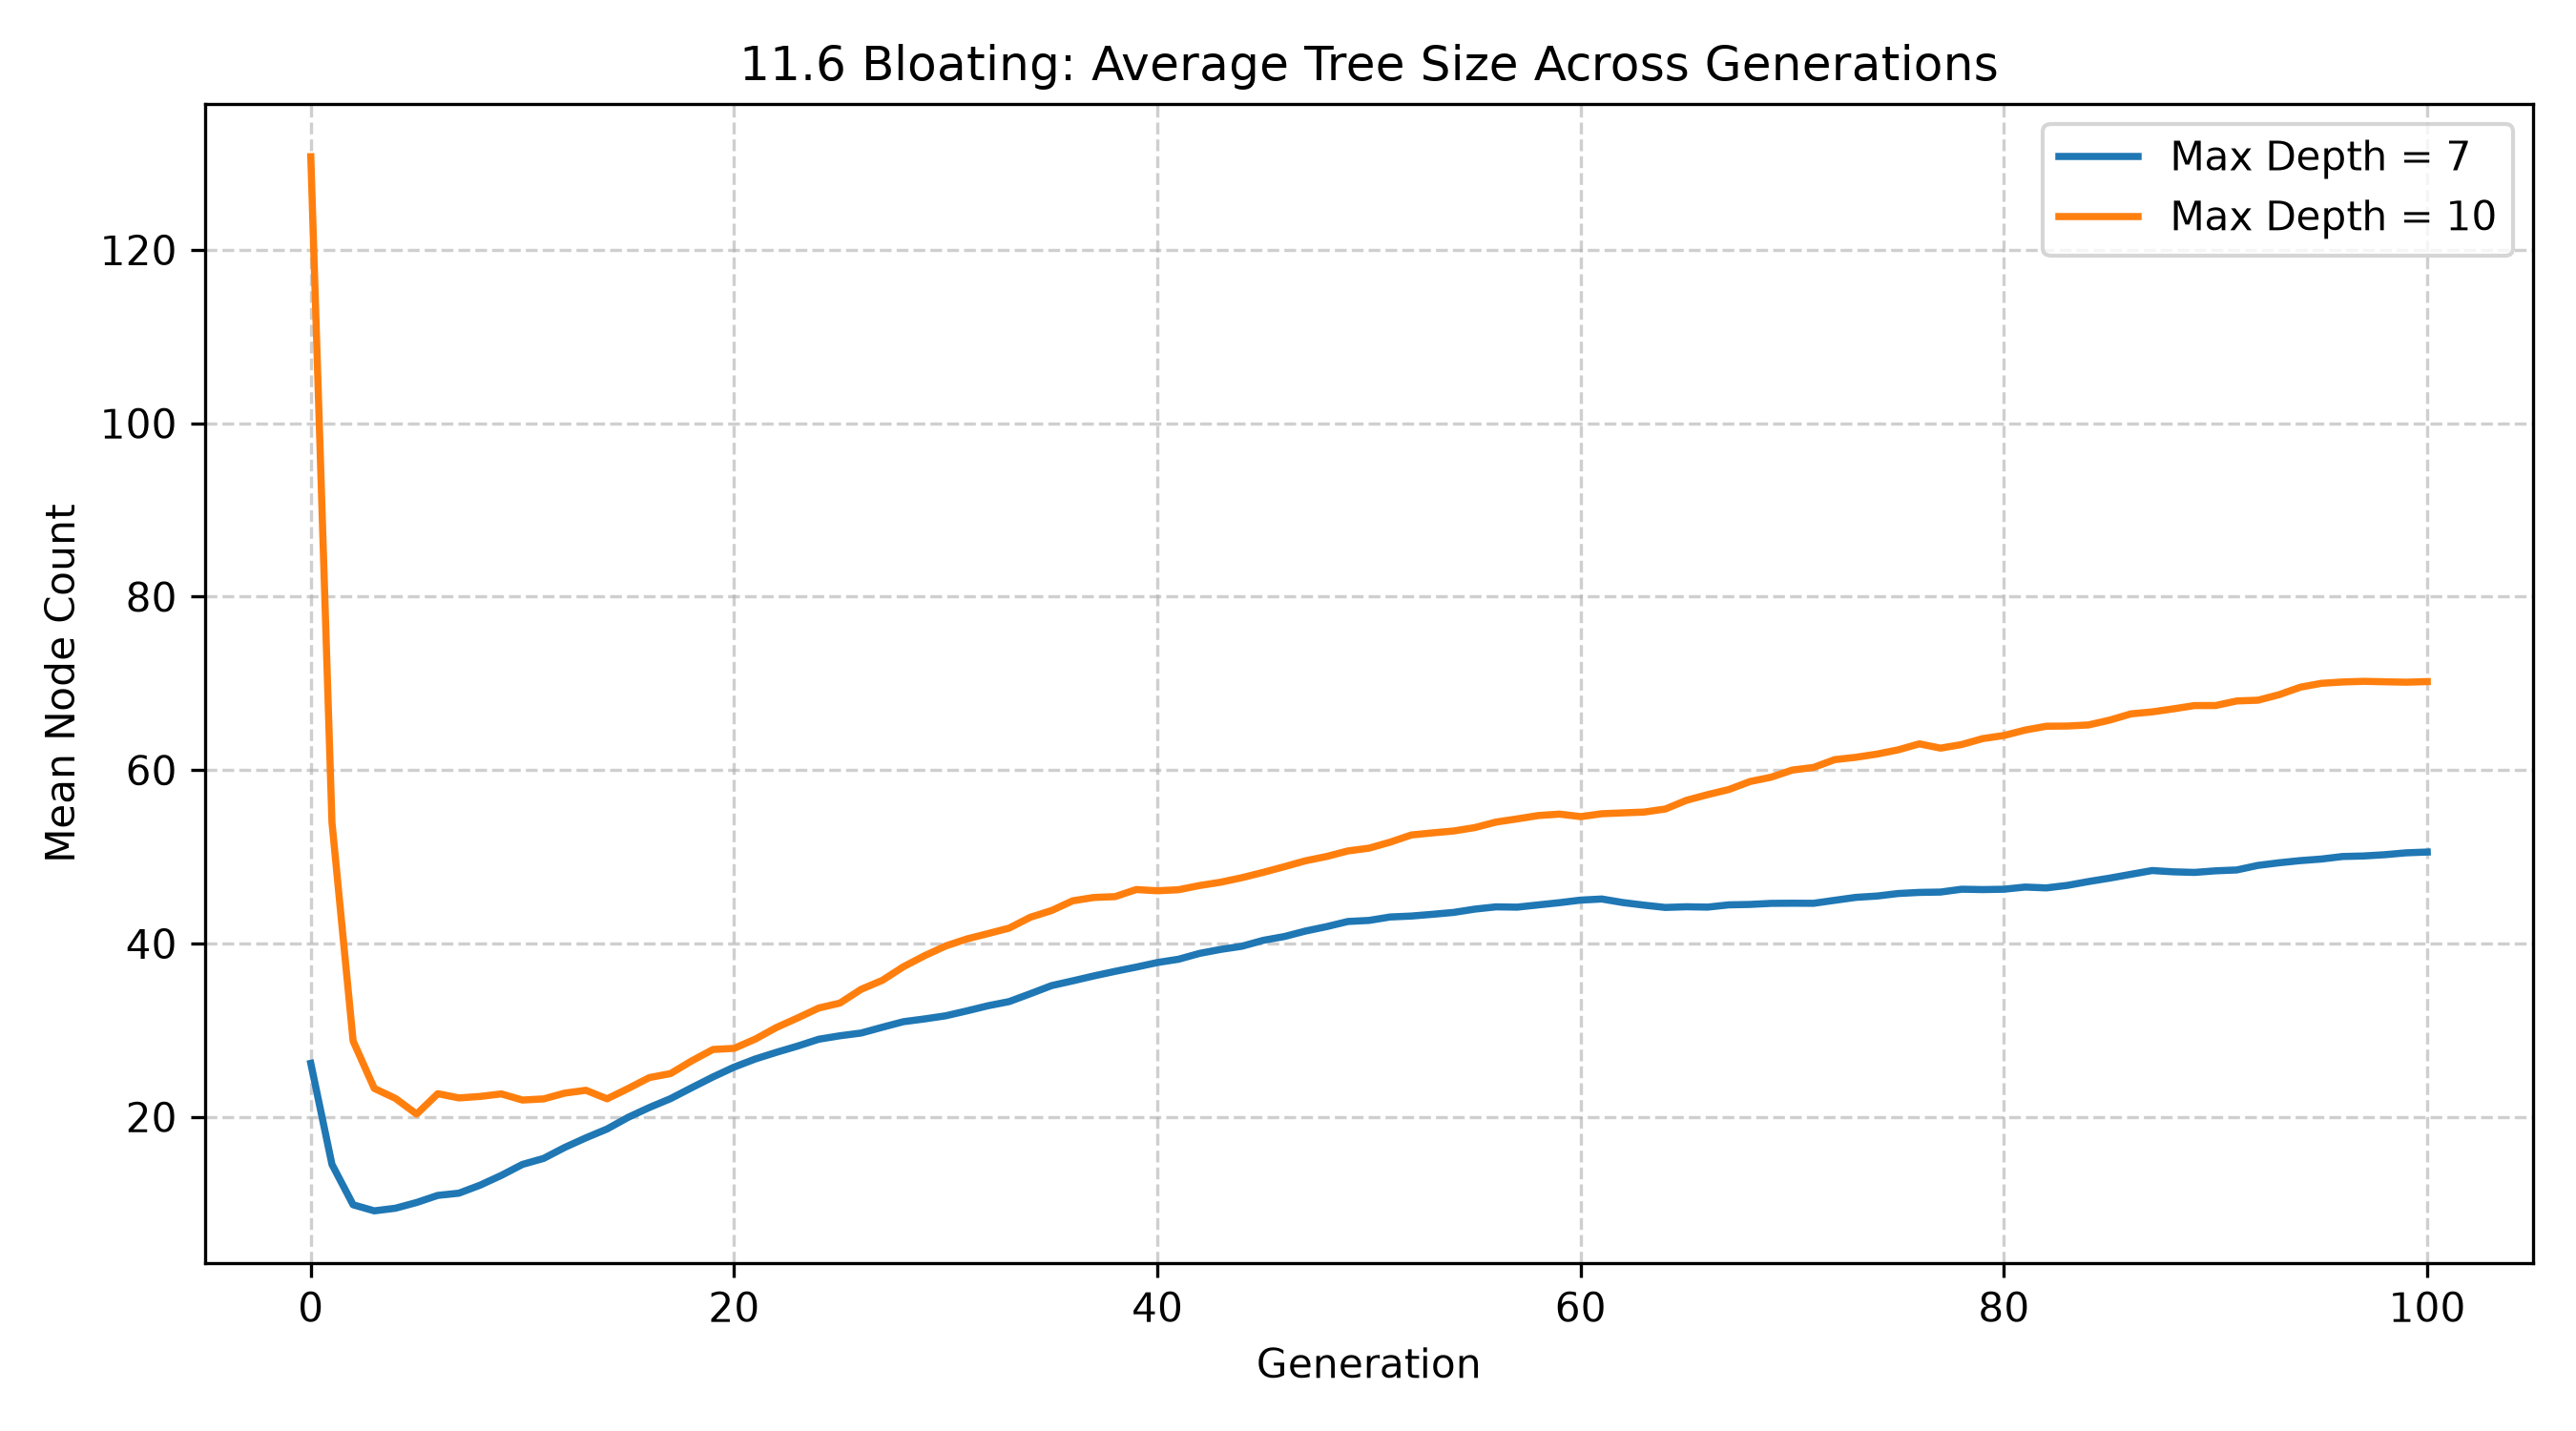
\includegraphics[width=0.75\linewidth]{bloating_depth_comparison.png}
  \caption{Evolução do tamanho médio da população com profundidade máxima 7 e 10.}
  \label{fig:f1_bloat}
\end{figure}

A \cref{tab:f1_bloat} e a \cref{fig:f1_bloat} mostram que o tamanho médio 
dobra em 100 gerações e cresce $2.5\times$ em 500 gerações, enquanto o
erro de treino praticamente não melhora depois da geração~80. Relaxar a
profundidade de 7 para 10 aumenta o tamanho do melhor indivíduo em $38\%$
($46.5\to64.4$ nós), sem ganho significativo de teste ($p=0.57$). As
expressões finais contêm \emph{introns} evidentes (por exemplo,
$x_0-x_0$ e $x_0/x_0$; ver \cref{app:expressoes}), por tanto, o limite de profundidade 7
funciona como regularizador estrutural, mas \textbf{não impede} o
\emph{bloat}.

% -----------------------------------------------------------------------------
\subsubsection{Replicação no \code{synth2} e no \code{concrete1}}
\label{sec:f1_replicacao}

\begin{table}[htbp]
  \centering
  \caption{Replicação da configuração da Fase~1 (torneio $k=2$, $\pc=0.9$,
           $\pmut=0.05$) nas demais bases.}
  \label{tab:f1_replicacao}
  \small
  \begin{tabular}{@{}lcccccc@{}}
    \toprule
    Base & RMSE treino & RMSE teste & Mediana & Máx. teste & Tam. melhor & $R^2_{\text{teste}}$ \\
    \midrule
    \code{synth1}               & $3.69 \pm 2.19$  & $5.52 \pm 4.89$   & 4.28  & 21.44  & $46.5 \pm 17.5$ & 0.95 \\
    \code{synth2}               & $2.66 \pm 0.38$  & $24.97 \pm 80.39$ & 3.47  & \textbf{415.26} & $48.0 \pm 11.6$ & $<0$ \\
    \code{concrete1} (bruto)    & $14.28 \pm 1.36$ & $13.97 \pm 1.44$  & 13.36 & 17.82  & $41.9 \pm 20.5$ & 0.26 \\
    \code{concrete1} (z-score)  & $12.39 \pm 1.45$ & $11.97 \pm 1.51$  & 11.65 & 16.67  & $74.1 \pm 27.2$ & 0.46 \\
    \bottomrule
  \end{tabular}
\end{table}

\begin{figure}[htbp]
  \centering
  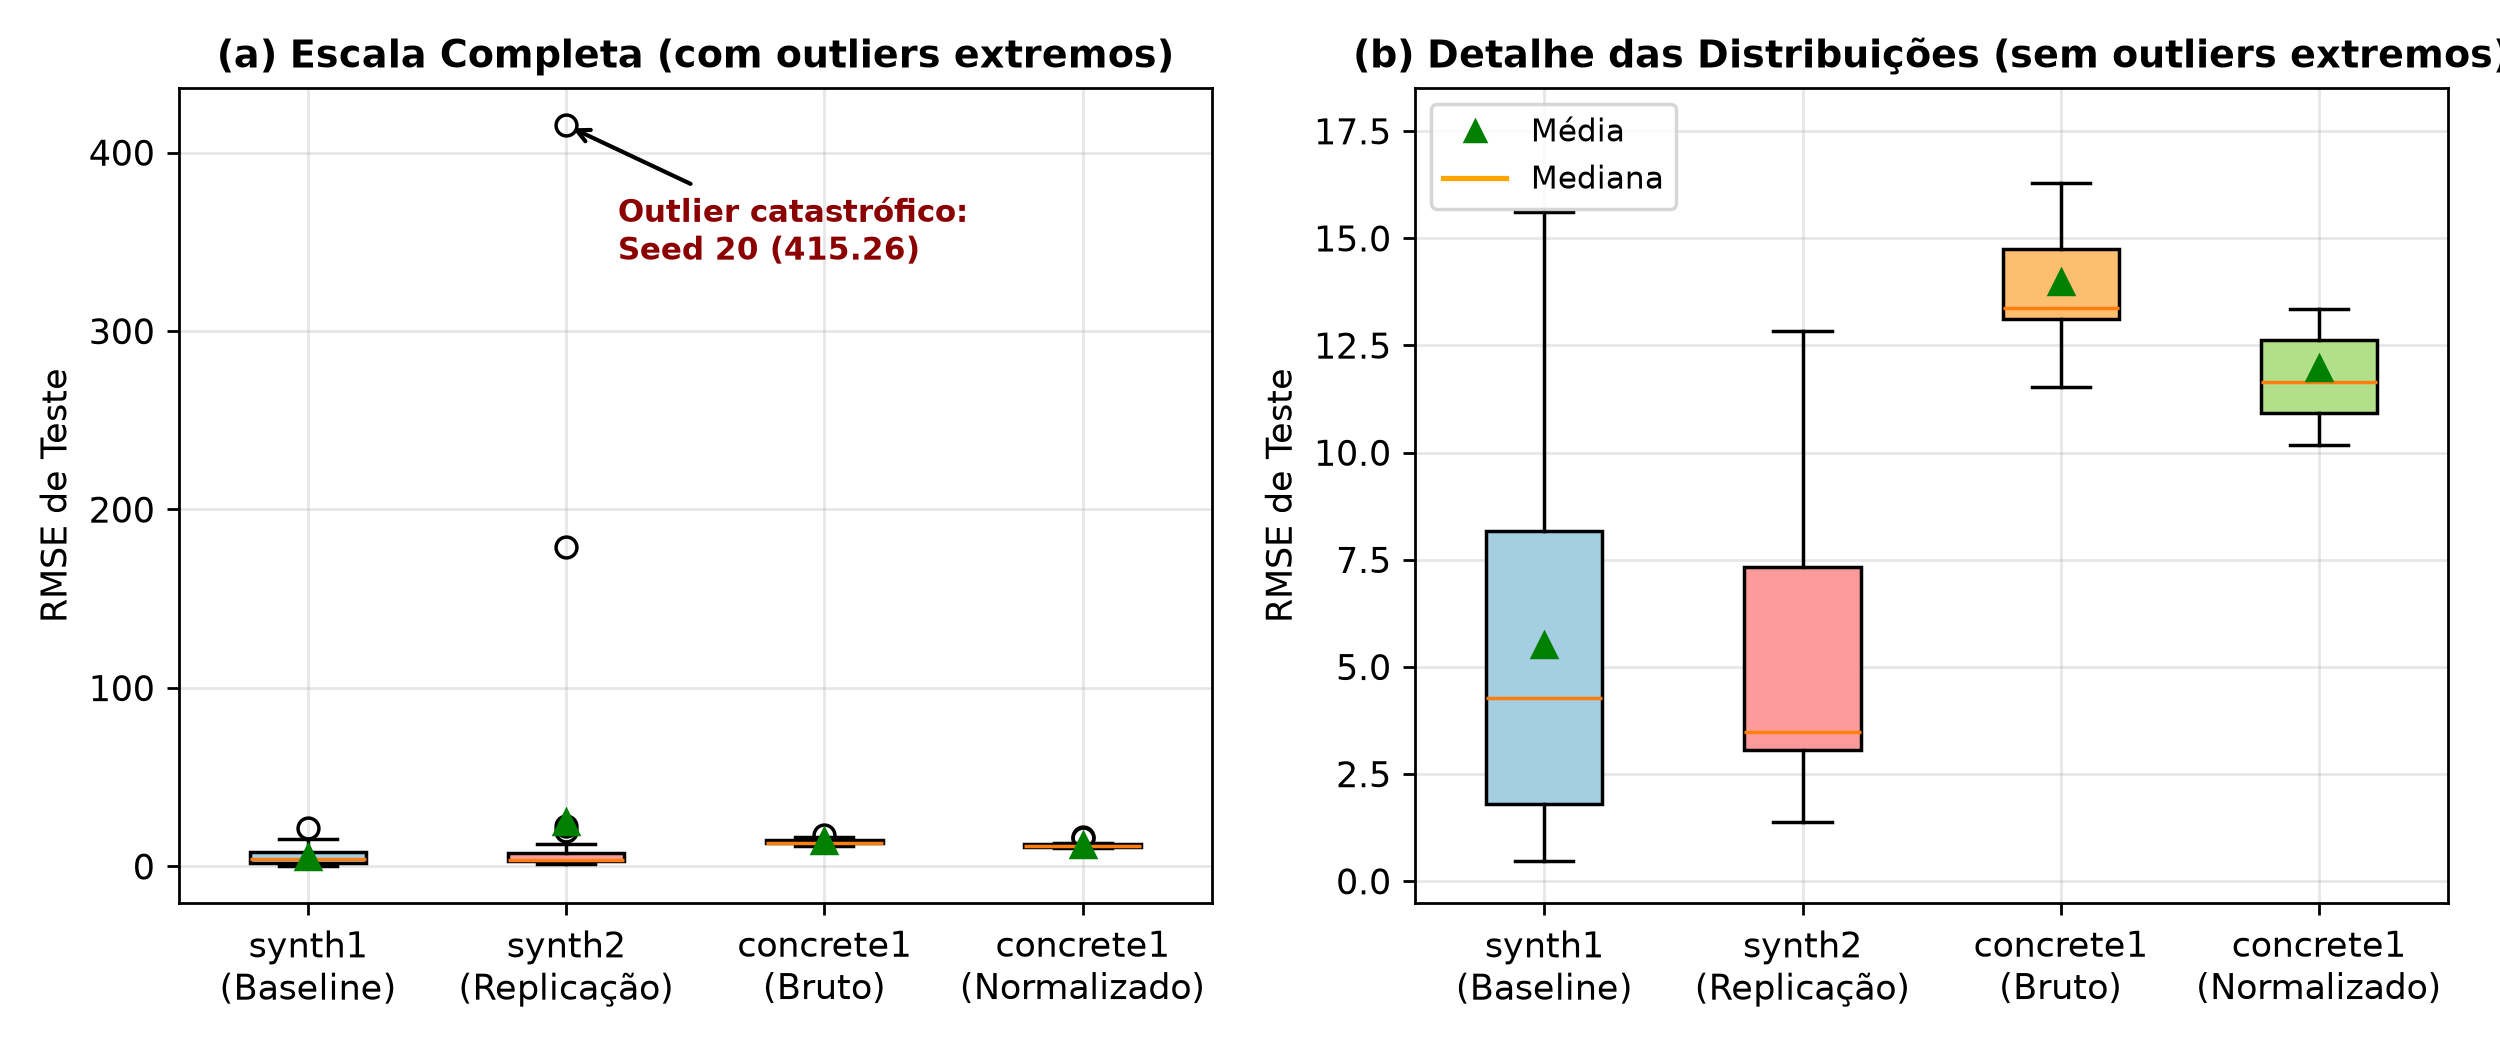
\includegraphics[width=\linewidth]{replication_all_datasets_two_panels.png}
  \caption{Desempenho da replicação da Fase~1 nas três bases (RMSE de teste, 30 execuções).
           O painel (a) exibe a escala completa, destacando os \emph{outliers} catastróficos
           do \code{synth2} decorrentes da divisão protegida clássica. O painel (b) apresenta
           o detalhe das distribuições (com corte de \emph{outliers} extremos fora de $[-0.5, 18.5]$),
           tornando claramente visíveis as medianas (linhas laranjas), médias (triângulos verdes)
           e a dispersão interquartil de todas as bases.}
  \label{fig:f1_replicacao}
\end{figure}

A replicação (\cref{tab:f1_replicacao,fig:f1_replicacao}) revelou
comportamentos qualitativamente diferentes entre as bases:

\begin{itemize}
  \item \textbf{\code{synth2}: sobreajuste catastrófico fora da amostra.}
        Conforme ilustrado no painel~(a) da \cref{fig:f1_replicacao}, embora o
        erro de treino seja baixo e estável ($2.66\pm0.38$), o erro de teste
        explode em 6 das 30 execuções (RMSE $>10$), culminando no valor extremo
        de $415.26$ na semente~20 (e $179.3$ na semente~21). Essa distorção
        comprime visualmente as caixas das demais bases. A inspeção analítica
        mostra que as expressões geraram divisões cujo denominador se aproxima
        de zero \emph{entre} os pontos de treino (ex.: $x_0/(x_0+x_1)$, que se
        anula sobre a reta $x_0 = -x_1$). Como a divisão de Koza (\cref{eq:div})
        só atua para $|b| < 10^{-6}$, qualquer denominador pequeno superior a
        esse limiar produz assíntotas gigantescas no teste.
  \item \textbf{\code{concrete1}: subajuste estrutural e ganho por normalização.}
        Graças ao painel detalhado~(b) da \cref{fig:f1_replicacao}, constata-se
        nitidamente que os erros de treino e teste são muito próximos ($12.4$ e
        $12.0$), descartando sobreajuste, mas indicando subajuste
        ($R^2 \approx 0.46$). Observa-se com clareza o benefício da
        normalização \emph{z-score} dos atributos de entrada frente aos dados
        brutos: a mediana cai de $13.36$ para $11.65$ e a média de $13.97$
        para $11.97$, com ganho estatisticamente significativo
        ($U = 786.0$, $p = 7.04\times10^{-7}$). Contudo, as árvores incham até
        74 nós para sintetizar a magnitude elevada da resposta ($\bar{y} \approx 35.8$); ver
        \cref{app:expressoes}.
  \item \textbf{\code{synth1}: consistência com gap moderado.} O painel~(b)
        evidencia que a distribuição do \code{synth1} concentra a maioria das
        sementes na faixa de 0 a 8 (mediana $4.28$), apresentando razão
        mediana teste/treino de $1.34$, plenamente compatível com o reduzido
        volume amostral de treino (60 amostras).
\end{itemize}

% -----------------------------------------------------------------------------
\subsubsection{Síntese da Fase 1 e questões em aberto}
\label{sec:f1_sintese}

\begin{table}[htbp]
  \centering
  \caption{Respostas da Fase~1 às questões do enunciado.}
  \label{tab:f1_sintese}
  \small
  \begin{tabularx}{\linewidth}{@{}lX@{}}
    \toprule
    Questão & Resposta da Fase~1 \\
    \midrule
    População/gerações & 100/100: saturação na geração $\approx80$; mais orçamento ajuda, preferencialmente em população. \\
    Seleção            & $\eps$-lexicase é o único fator significativo ($p=4.1\times10^{-6}$); roleta $\approx$ torneio $k=2$; $k=3$ provoca convergência prematura. \\
    $\pc$ e $\pmut$    & \emph{Crossover} destrutivo em 89\% dos casos (em relação ao melhor pai); ótimo intermediário ($\pc\approx0.7$, $\pmut\approx0.1$) indicado, mas não testado em conjunto. \\
    Elitismo           & Necessário: sem ele, a mediana do teste dobra e as árvores crescem. \\
    \emph{Bloating}    & Medido pelo tamanho médio/melhor ao longo das gerações; fator de $1.9\times$ a $2.8\times$; o limite de profundidade não o impede. \\
    Treino $\times$ teste & \code{synth2}: explosões fora da amostra; \code{concrete1}: subajuste ($R^2\approx0.46$). \\
    \bottomrule
  \end{tabularx}
\end{table}

A \cref{tab:f1_sintese} resume as respostas. A Fase~1 deixou cinco sintomas
sem explicação mecanística, que motivam a Fase~2:
\textbf{(S1)}~explosões assintóticas no \code{synth2};
\textbf{(S2)}~\emph{crossover} destrutivo e ótimo de operadores não validado;
\textbf{(S3)}~10--27\% de clones por geração, mesmo com $\eps$-lexicase no
final da evolução;
\textbf{(S4)}~crescimento das árvores com \emph{introns}; e
\textbf{(S5)}~subajuste estrutural no \code{concrete1}. Além disso, a
$\eps$-lexicase só havia sido avaliada no \code{synth1}.

% =============================================================================
\subsection{Fase 2: Investigação Guiada pela \emph{Fitness Landscape}}
\label{sec:fase2}

A Fase~1 encerrou-se com resultados contundentes, porém revelou limitações
severas: o método de seleção $\eps$-lexicase mitigou o erro médio no
\code{synth1}, mas sua replicação direta no \code{synth2} manteve explosões
fora da amostra ($415.3$ de erro máximo no teste), enquanto no \code{concrete1}
o algoritmo permaneceu estagnado em subajuste estrutural ($R^2 \approx 0.45$).
Além disso, constatou-se que cerca de $89\%$ dos cruzamentos deterioram o
melhor pai, a população acumula duplicatas canônicas e o tamanho médio das
árvores dobra sob acúmulo de código neutro.

Na Fase~2, abandona-se o ajuste puramente empírico de hiperparâmetros e
adota-se uma metodologia orientada pelas propriedades da \textbf{\emph{fitness
landscape}}~\cite{wright1932roles}. Os sintomas observados na Fase~1 são
formalizados como patologias da topologia de busca e convertidos em seis
hipóteses mecanicistas (H1 a H6), avaliadas primeiro por \textbf{ablação
isolada} contra o estado atual e, em seguida, por \textbf{empilhamento
sequencial auditável}.

% -----------------------------------------------------------------------------
\subsubsection{Do Estado Atual (\cfg{S0}) às Hipóteses da Paisagem de Aptidão}
\label{sec:f2_hipoteses}

Para isolar o efeito das intervenções, definiu-se como ponto de partida o
\textbf{Estado Atual (\cfg{S0})}, que adota a $\eps$-lexicase com tolerância
MAD nas três bases, mantendo a parametrização canônica da Fase~1
(\code{pop=100}, \code{gen=100}, $\pc=0.9$, $\pmut=0.05$, profundidade máxima
7 e elitismo unitário). A \cref{tab:f2_diagnostico_s0} resume o desempenho de
\cfg{S0} e diagnostica as causas na paisagem.

\begin{table}[htbp]
  \centering
  \caption{Diagnóstico do Estado Atual (\cfg{S0}) com $\eps$-lexicase nas três
           bases (30 repetições).}
  \label{tab:f2_diagnostico_s0}
  \small
  \resizebox{\linewidth}{!}{%
  \begin{tabular}{@{}lccccp{7.5cm}@{}}
    \toprule
    Base & RMSE treino & RMSE teste & Mediana (IQR) & Tam. melhor & Diagnóstico do Estado Atual (\cfg{S0}) \\
    \midrule
    \code{synth1} & $0.99 \pm 1.21$ & $1.62 \pm 3.36$ & 0.68 (1.12) & $46.3 \pm 14.3$ &
    Excelente ganho sobre torneio, mas sofre com \emph{outliers} de teste (máx. 18.19) e introns algébricos. \\
    \code{synth2} & $2.11 \pm 0.36$ & $13.15 \pm 17.48$ & 5.72 (15.96) & $57.1 \pm 16.6$ &
    Reduz o erro médio pela metade, mas \textbf{persistem explosões assintóticas} fora da amostra (máx. 86.55). \\
    \code{concrete1} & $12.60 \pm 1.48$ & $12.19 \pm 1.59$ & 11.81 (2.20) & $59.8 \pm 18.8$ &
    Subajuste severo ($R^2 = 0.44$): dezenas de nós gastos somando constantes $[-1,1]$ rumo ao patamar médio de $y \approx 35.8$. \\
    \bottomrule
  \end{tabular}}
\end{table}

A partir desse diagnóstico, estabeleceu-se a matriz de hipóteses detalhada na
\cref{tab:f2_matriz_hipoteses}, associando cada dado empírico da Fase~1 a uma
propriedade da paisagem e à sua respectiva intervenção algorítmica.

\begin{table}[htbp]
  \centering
  \caption{Cadeia metodológica: Sintoma empírico $\to$ Propriedade da
           \emph{Fitness Landscape} $\to$ Intervenção Algorítmica.}
  \label{tab:f2_matriz_hipoteses}
  \small
  \begin{tabularx}{\linewidth}{@{}c>{\raggedright\arraybackslash}p{4.0cm}XX@{}}
    \toprule
    Hip. & Sintoma da Fase 1 & Propriedade da Paisagem & Intervenção Proposta \\
    \midrule
    \textbf{H1} & Erro de teste explode no \code{synth2} (máx. 415.3 na F1, 86.6 no \cfg{S0}). &
    \textbf{Polos e Falésias:} a divisão protegida ($\mathrm{div}(a,b)=1$ para $|b|<10^{-6}$) cria assíntotas quase verticais entre os pontos de treino. &
    Substituição de \code{div} pelo \textbf{Analytic Quotient} ($\mathrm{aq}(a,b) = a/\sqrt{1+b^2}$), infinitamente diferenciável. \\
    \addlinespace[3pt]
    \textbf{H2} & $>88\%$ dos cruzamentos geram filhos piores que os pais; mutação tem alta eficiência local. &
    \textbf{Rugosidade e Epistasia Estrutural:} troca de subárvores atua como macromutação destrutiva que destrói blocos contextuais. &
    Rebalanceamento ($\pc=0.7$, $\pmut=0.15$) com \textbf{mutação mista} (35\% Gaussiana em ERC, 35\% pontual, 30\% subárvore). \\
    \addlinespace[3pt]
    \textbf{H3} & 10\% a 27\% da população em cada geração é composta por clones canônicos (\code{n\_repeated}). &
    \textbf{Vales e Perda de Diversidade:} acúmulo de clones no fundo de bacias reduz \emph{stepping stones} disponíveis para a $\eps$-lexicase. &
    \textbf{Rejeição/diversificação de duplicatas} (\code{dedup}): filhos idênticos a membros da geração sofrem mutação obrigatória. \\
    \addlinespace[3pt]
    \textbf{H4} & Alta dispersão entre sementes aleatórias; estagnação em bacias de atração subótimas. &
    \textbf{Multimodalidade:} populações panmíticas convergem para uma única bacia atratora prematuramente. &
    \textbf{Modelo de Ilhas} (4 subpopulações de 25 indivíduos) com migração em anel periódica (2 elites a cada 20 gerações). \\
    \addlinespace[3pt]
    \textbf{H5} & Crescimento das árvores até 50--74 nós acumulando introns ($x_0-x_0$, $x_0/x_0$). &
    \textbf{Redes Neutras de Bloat:} árvores infladas mantêm idêntica aptidão de treino, mas degradam generalização. &
    \textbf{Parcimônia Lexicográfica}: desempate de candidatos sobreviventes na $\eps$-lexicase priorizando menor número de nós. \\
    \addlinespace[3pt]
    \textbf{H6} & \code{concrete1} estagnado em $R^2 \approx 0.44$; gasto massivo de nós para ajustar escala. &
    \textbf{Barreira de Escala e Subexpressividade:} busca simultânea de forma e escala; operadores puramente aritméticos são ineficientes para modelar curvaturas e saturações não-lineares. &
    \textbf{H6a:} \emph{Linear Scaling} ótimo via OLS ($\hat{y} = \alpha + \beta g(X)$); \textbf{H6b:} expansão para $\mathcal{F}=\{+,-,\times,\mathrm{aq},\log,\sqrt,\exp\}$. \\
    \bottomrule
  \end{tabularx}
\end{table}

\newpage

% -----------------------------------------------------------------------------
\subsubsection{Avaliação das Hipóteses: Metodologia de Ablação e Escadas}
\label{sec:f2_ablacao}

\paragraph{Racional Metodológico: Por que Ablação e Escadas em vez de Busca Fatorial?}
Com seis eixos de intervenção algorítmica (H1 a H6b), um projeto fatorial exaustivo
exigiria avaliar todas as $2^6 = 64$ combinações possíveis. Considerando as três
bases de dados e 30 repetições com sementes independentes pareadas, isso
demandaria $64 \times 3 \times 30 = 5\,760$ execuções completas, tornando o processo
computacionalmente proibitivo e metodologicamente cego (ao explorar arranjos
conceitualmente inconsistentes).

Para contornar essa barreira combinatória, adotou-se o protocolo padrão da
literatura de aprendizado de máquina e computação natural em duas etapas:
\begin{enumerate}
  \item \textbf{Ablação Isolada ($1 \times 1$ contra \cfg{S0}):} avalia-se a
        contribuição líquida e os efeitos colaterais de cada hipótese individualmente;
        intervenções que aumentam a dispersão ou geram custo proibitivo sem ganho
        estatístico (como o Modelo de Ilhas H4) são descartadas (\emph{pruned}) da
        linhagem de desenvolvimento;
  \item \textbf{Empilhamento Cumulativo em Escadas:} as hipóteses aprovadas são
        integradas progressivamente em duas linhagens lógicas (a Escada~A para problemas
        polinomiais e a Escada~B para problemas numéricos com descontinuidades e
        desacoplamento de escala), avaliando o ganho marginal de cada adição.
\end{enumerate}

Na etapa de ablação isolada, cada hipótese foi avaliada individualmente contra
\cfg{S0} ao longo de 30 repetições pareadas por semente nas três bases
(\cref{tab:f2_ablacao}). Para evidenciar o impacto relativo, a \cref{fig:f2_heatmap}
ilustra a razão entre a mediana do RMSE de cada hipótese e a mediana do \cfg{S0}.

\begin{table}[htbp]
  \centering
  \caption{Ablação isolada das hipóteses H1 a H6b contra o Estado Atual (\cfg{S0}).
           Valores de $p$ referem-se ao teste pareado de Wilcoxon ($p_W$) e
           Mann--Whitney ($p_{MW}$). W/L indica Vitórias/Derrotas por semente.}
  \label{tab:f2_ablacao}
  \small
  \resizebox{\linewidth}{!}{%
  \begin{tabular}{@{}llccccccc@{}}
    \toprule
    Base & Configuração & RMSE treino & RMSE teste & Mediana (IQR) & Tam. & W/L vs \cfg{S0} & $p_W$ & $p_{MW}$ \\
    \midrule
    \multirow{8}{*}{\code{synth1}}
    & \cfg{S0}: Estado Atual & $0.99 \pm 1.21$ & $1.62 \pm 3.36$ & 0.68 (1.12) & $46.3 \pm 14.3$ & --- & --- & --- \\
    & \cfg{H1} (AQ)           & $1.22 \pm 1.31$ & $2.02 \pm 2.21$ & 1.31 (1.44) & $64.0 \pm 19.2$ & 12W / 18L & 0.124 & 0.042 \\
    & \cfg{H2} (Operadores)   & $0.85 \pm 1.14$ & $1.17 \pm 2.47$ & \textbf{0.25 (1.17)} & $40.7 \pm 14.3$ & 18W / 12L & 0.670 & 0.090 \\
    & \cfg{H3} (Dedup)        & $0.65 \pm 0.71$ & \textbf{0.78 $\pm$ 1.50} & 0.41 (0.77) & $47.0 \pm 17.3$ & 17W / 13L & 0.171 & 0.112 \\
    & \cfg{H4} (Ilhas)        & $1.31 \pm 0.94$ & $1.33 \pm 1.55$ & 1.28 (0.56) & $38.8 \pm 20.0$ & 10W / 20L & 0.184 & 0.088 \\
    & \cfg{H5} (Parcimônia)   & $0.79 \pm 0.59$ & \textbf{0.76 $\pm$ 0.57} & 0.72 (0.98) & \textbf{41.1 $\pm$ 14.0} & 15W / 15L & 0.598 & 0.600 \\
    & \cfg{H6a} (Scaling)     & $1.10 \pm 1.31$ & $2.05 \pm 2.89$ & 1.10 (1.96) & $57.8 \pm 19.0$ & 12W / 18L & 0.177 & 0.318 \\
    & \cfg{H6b} (Não-lin+Scal)& $1.37 \pm 0.49$ & $2.23 \pm 1.03$ & 2.24 (0.99) & $41.0 \pm 13.7$ & 4W / 26L  & 0.003 & $7.7{\times}10^{-5}$ \\
    \midrule
    \multirow{8}{*}{\code{synth2}}
    & \cfg{S0}: Estado Atual & $2.11 \pm 0.36$ & $13.15 \pm 17.48$ & 5.72 (15.96) & $57.1 \pm 16.6$ & --- & --- & --- \\
    & \cfg{H1} (AQ)           & $1.93 \pm 0.26$ & \textbf{2.29 $\pm$ 0.39} & \textbf{2.34 (0.27)} & $67.4 \pm 18.5$ & \textbf{25W / 5L} & $\mathbf{1.1{\times}10^{-5}}$ & $\mathbf{2.2{\times}10^{-6}}$ \\
    & \cfg{H2} (Operadores)   & $2.05 \pm 0.40$ & $12.12 \pm 15.12$ & 5.28 (15.69) & $48.8 \pm 13.2$ & 19W / 11L & 0.641 & 0.610 \\
    & \cfg{H3} (Dedup)        & $2.08 \pm 0.45$ & $17.32 \pm 20.34$ & 11.78 (24.66) & $51.9 \pm 15.4$ & 16W / 14L & 0.556 & 0.982 \\
    & \cfg{H4} (Ilhas)        & $2.45 \pm 0.36$ & $12.38 \pm 14.20$ & 3.47 (17.68) & $44.4 \pm 18.6$ & 15W / 15L & 0.792 & 0.819 \\
    & \cfg{H5} (Parcimônia)   & $2.01 \pm 0.34$ & $26.40 \pm 49.67$ & 6.64 (23.24) & $50.8 \pm 15.5$ & 14W / 16L & 0.177 & 0.751 \\
    & \cfg{H6a} (Scaling)     & $1.41 \pm 0.12$ & \textbf{1.72 $\pm$ 1.13} & \textbf{1.40 (0.29)} & $57.5 \pm 23.0$ & \textbf{29W / 1L} & $\mathbf{3.9{\times}10^{-7}}$ & $\mathbf{1.1{\times}10^{-9}}$ \\
    & \cfg{H6b} (Não-lin+Scal)& $1.69 \pm 0.24$ & $2.08 \pm 0.50$ & 2.03 (0.53) & $39.5 \pm 9.2$ & 26W / 4L & $1.0{\times}10^{-7}$ & $7.0{\times}10^{-7}$ \\
    \midrule
    \multirow{8}{*}{\code{concrete1}}
    & \cfg{S0}: Estado Atual & $12.60 \pm 1.48$ & $12.19 \pm 1.59$ & 11.81 (2.20) & $59.8 \pm 18.8$ & --- & --- & --- \\
    & \cfg{H1} (AQ)           & $15.76 \pm 5.59$ & $15.78 \pm 5.84$ & 12.66 (10.46) & $95.9 \pm 17.8$ & 14W / 16L & 0.020 & 0.240 \\
    & \cfg{H2} (Operadores)   & $13.29 \pm 2.83$ & $13.02 \pm 3.05$ & 12.32 (2.44) & $58.1 \pm 21.2$ & 14W / 16L & 0.371 & 0.420 \\
    & \cfg{H3} (Dedup)        & $12.17 \pm 1.18$ & $11.74 \pm 1.18$ & 11.57 (1.78) & $54.3 \pm 15.0$ & 17W / 13L & 0.280 & 0.304 \\
    & \cfg{H4} (Ilhas)        & $13.32 \pm 1.42$ & $12.91 \pm 1.44$ & 12.87 (1.92) & $54.9 \pm 20.0$ & 10W / 20L & 0.067 & 0.068 \\
    & \cfg{H5} (Parcimônia)   & $12.42 \pm 1.44$ & $12.97 \pm 6.27$ & 11.74 (1.61) & $59.4 \pm 21.2$ & 16W / 13L & 0.721 & 0.605 \\
    & \cfg{H6a} (Scaling)     & $\mathbf{9.14 \pm 0.71}$ & $\mathbf{8.90 \pm 0.65}$ & \textbf{8.79 (0.77)} & $57.5 \pm 10.5$ & \textbf{30W / 0L} & $\mathbf{1.9{\times}10^{-9}}$ & $\mathbf{9.9{\times}10^{-11}}$ \\
    & \cfg{H6b} (Não-lin+Scal)& $\mathbf{7.75 \pm 0.40}$ & $\mathbf{7.61 \pm 0.53}$ & \textbf{7.51 (0.56)} & \textbf{49.4 $\pm$ 9.7} & \textbf{30W / 0L} & $\mathbf{1.9{\times}10^{-9}}$ & $\mathbf{3.0{\times}10^{-11}}$ \\
    \bottomrule
  \end{tabular}}
\end{table}

\newpage

\begin{figure}[htbp]
  \centering
  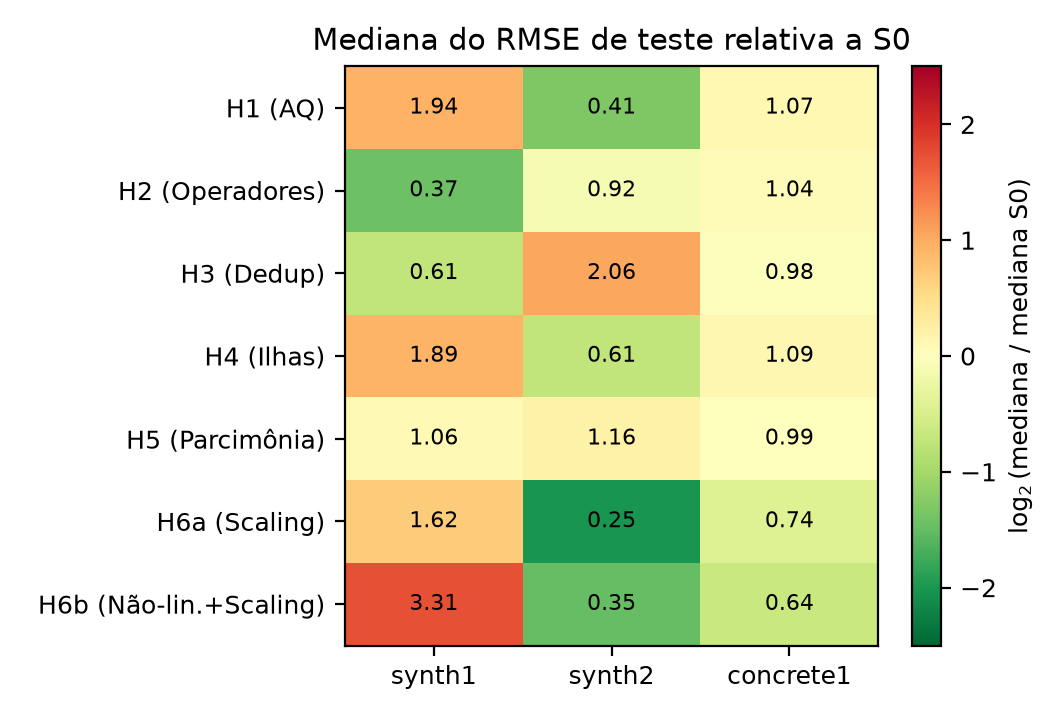
\includegraphics[width=0.58\linewidth]{f2_heatmap_hipoteses.png}
  \caption{Heatmap do impacto relativo das hipóteses isoladas. Valores indicam
           a razão entre a mediana do RMSE de teste da hipótese e a mediana de \cfg{S0}
           (valores $<1.0$ indicam melhoria sobre o estado atual).}
  \label{fig:f2_heatmap}
\end{figure}

A análise estatística isolada conduz a vereditos categóricos:

\begin{enumerate}
  \item \textbf{H1 (Analytic Quotient): Aprovada com sinergia necessária.} No
        \code{synth2}, o AQ teve impacto espetacular: reduziu o RMSE de teste
        de $13.15$ para $2.29$, derrubou a mediana para $2.34$ e o erro máximo
        de $86.55$ para $3.59$ ($25$ vitórias em 30 sementes,
        $p_W = 1.1\times10^{-5}$), eliminando 100\% das singularidades
        assintóticas. Contudo, no \code{concrete1} isolado, o AQ degradou o
        erro ($12.19 \to 15.78$). A razão matemática é direta: como
        $|\mathrm{aq}(a,b)| \le |a|$, o operador limita a magnitude da saída;
        sem constantes $>35$, a árvore não consegue alcançar o patamar da base
        empírica sem \emph{Linear Scaling}. Portanto, H1 requer acoplamento
        com H6a em problemas não normalizados em $y$.
  \item \textbf{H2 (Rebalanceamento $\pc=0.7,\pmut=0.15$ + Mutação Mista):
        Aprovada.} Reduziu a mediana do erro no \code{synth1} em mais de $63\%$
        ($0.68 \to 0.25$) e encolheu o tamanho médio de $46.3$ para $40.7$ nós.
        A perturbação gaussiana nas ERC permite navegação suave nas encostas
        contínuas das bacias de atração, sem desmantelar os blocos sintáticos.
  \item \textbf{H3 (Rejeição de Duplicatas): Aprovada.} No \code{synth1},
        reduziu o erro médio pela metade ($1.62 \to 0.78$) e a mediana para
        $0.41$. Impedir que clones saturem a população preserva nichos para a
        filtragem da $\eps$-lexicase.
  \item \textbf{H4 (Modelo de Ilhas $4\times25$): Rejeitada para \code{pop=100}.}
        Embora tenha reduzido o tamanho das árvores, o modelo piorou o erro de
        teste no \code{synth1} (20 derrotas) e no \code{concrete1} (20
        derrotas). O motivo reside na mecânica da seleção: a $\eps$-lexicase
        necessita de um conjunto diversificado de candidatos para sustentar
        especialistas em múltiplos casos de teste. Ao fatiar a população em
        subpopulações de apenas 25 indivíduos, a diversidade interna colapsa
        antes da migração. O modelo de ilhas foi descartado do empilhamento.
  \item \textbf{H5 (Parcimônia Lexicográfica): Aprovada como antídoto de bloat.}
        No \code{synth1}, reduziu o erro médio de teste de $1.62$ para $0.76$ e
        despencou o erro máximo de $18.19$ para $2.07$, enxugando as árvores
        para $41.1$ nós. O desempate por tamanho elimina o código neutro sem
        impor perda de capacidade expressiva.
  \item \textbf{H6 (Linear Scaling e Primitivas Não-Lineares): Aprovada com
        impacto extremo.} No \code{concrete1}, o \emph{Linear Scaling} (H6a)
        venceu \cfg{S0} em \textbf{30 de 30 sementes}
        ($p_W = 1.9\times10^{-9}$), reduzindo o RMSE para $8.90$. Ao adicionar
        as funções unárias $\{ \log, \sqrt, \exp \}$ (H6b), o erro caiu para
        $7.61$ com $R^2 = 0.78$ ($30/30$ vitórias, $p_W = 1.9\times10^{-9}$)
        e o tamanho médio caiu para $49.4$ nós. No \code{synth2}, H6a também
        obteve 29 vitórias em 30 sementes ($p_W = 3.9\times10^{-7}$).
\end{enumerate}

% -----------------------------------------------------------------------------
\subsubsection{Empilhamento Sequencial: As Duas Escadas Auditáveis}
\label{sec:f2_empilhamento}

Com as hipóteses validadas individualmente (e descartada H4), estruturou-se um
processo de empilhamento cumulativo em duas trajetórias metodológicas:

\begin{itemize}
  \item \textbf{Escada A (Estrutural / Algébrica Pura):} direcionada a
        problemas polinomiais exatos sem necessidade de reescalonamento contínuo:
        \[
          \cfg{S0} \longrightarrow \cfg{Stack~A1}\ (+\mathrm{H3} + \mathrm{H5})
          \longrightarrow \cfg{Stack~A2}\ (+\mathrm{H2\ Operadores}).
        \]
  \item \textbf{Escada B (Numérica / Físico-Química Completa):} concebida
        para superfícies racionais e problemas reais de engenharia:
        \begin{align*}
          \cfg{S0} &\longrightarrow \cfg{Stack~B1}\ (+\mathrm{H6a\ Scaling} + \mathrm{H1\ AQ})
          \longrightarrow \cfg{Stack~B2}\ (+\mathrm{H3} + \mathrm{H5}) \\
          &\longrightarrow \cfg{Stack~B3}\ (+\mathrm{H2\ Operadores})
          \longrightarrow \cfg{Stack~B4}\ (+\mathrm{H6b\ Não-Lineares}).
        \end{align*}
\end{itemize}

A \cref{tab:f2_escadas} detalha a progressão estatística ao longo das etapas,
enquanto a \cref{fig:f2_escadas} ilustra as curvas de transição do estado
inicial da Fase~1 até o ápice da Fase~2.

\begin{table}[htbp]
  \centering
  \caption{Progressão das Escadas de Empilhamento A e B nas três bases (30 repetições).}
  \label{tab:f2_escadas}
  \small
  \resizebox{\linewidth}{!}{%
  \begin{tabular}{@{}llccccccc@{}}
    \toprule
    Base & Etapa do Empilhamento & RMSE treino & RMSE teste & Mediana (IQR) & Mín./Máx. & Tam. melhor & W/L vs \cfg{S0} & $p_W$ \\
    \midrule
    \multirow{5}{*}{\code{synth1}}
    & Fase 1 (Torneio $k=2$)       & $3.69 \pm 2.19$ & $5.52 \pm 4.89$ & 4.28 (6.38) & 0.46 / 21.44 & $46.5 \pm 17.5$ & --- & --- \\
    & \cfg{S0}: Estado Atual       & $0.99 \pm 1.21$ & $1.62 \pm 3.36$ & 0.68 (1.12) & 0.01 / 18.19 & $46.3 \pm 14.3$ & Ref. & Ref. \\
    & \cfg{Stack~A1} (Dedup+Parc.) & $0.57 \pm 0.52$ & $0.64 \pm 0.62$ & 0.43 (0.72) & 0.04 / 2.38  & $43.8 \pm 16.2$ & 19W / 11L & 0.109 \\
    & \textbf{\cfg{Stack~A2}} (+Operadores) & $\mathbf{0.62 \pm 1.22}$ & $\mathbf{0.69 \pm 1.81}$ & $\mathbf{0.093\ (0.76)}$ & $\mathbf{0.0006}$ / 9.93 & $\mathbf{35.9 \pm 11.5}$ & \textbf{23W / 7L} & $\mathbf{1.1{\times}10^{-3}}$ \\
    & \cfg{Stack~B3} (Global)      & $0.91 \pm 1.05$ & $1.59 \pm 1.82$ & 1.35 (1.88) & 0.0001 / 8.51 & $55.6 \pm 17.1$ & 11W / 19L & 0.262 \\
    \midrule
    \multirow{6}{*}{\code{synth2}}
    & Fase 1 (Torneio $k=2$)       & $2.66 \pm 0.38$ & $24.97 \pm 80.39$ & 3.47 (4.26) & 1.39 / 415.26 & $48.0 \pm 11.6$ & --- & --- \\
    & \cfg{S0}: Estado Atual       & $2.11 \pm 0.36$ & $13.15 \pm 17.48$ & 5.72 (15.96) & 1.56 / 86.55 & $57.1 \pm 16.6$ & Ref. & Ref. \\
    & \cfg{Stack~B1} (Scaling+AQ)  & $1.41 \pm 0.14$ & $1.62 \pm 0.41$ & 1.49 (0.35) & 1.34 / 3.38  & $74.1 \pm 26.0$ & 29W / 1L & $1.6\times10^{-7}$ \\
    & \cfg{Stack~B2} (+Dedup+Parc.)& $1.45 \pm 0.18$ & $1.61 \pm 0.31$ & 1.47 (0.38) & 1.32 / 2.41  & $68.3 \pm 27.4$ & 29W / 1L & $1.3\times10^{-8}$ \\
    & \textbf{\cfg{Stack~B3}} (+Operadores) & $\mathbf{1.39 \pm 0.14}$ & $\mathbf{1.52 \pm 0.26}$ & $\mathbf{1.43\ (0.20)}$ & 1.28 / \textbf{2.35} & $\mathbf{61.6 \pm 28.2}$ & \textbf{30W / 0L} & $\mathbf{1.9{\times}10^{-9}}$ \\
    & \cfg{Stack~B4} (+Não-Lin.)   & $1.62 \pm 0.24$ & $1.89 \pm 0.32$ & 1.87 (0.56) & 1.37 / 2.48  & $42.4 \pm 13.6$ & 27W / 3L & $4.7\times10^{-8}$ \\
    \midrule
    \multirow{6}{*}{\code{concrete1}}
    & Fase 1 (Torneio $k=2$)       & $12.39 \pm 1.45$ & $11.97 \pm 1.51$ & 11.65 (1.72) & 10.18 / 16.67 & $74.1 \pm 27.2$ & --- & --- \\
    & \cfg{S0}: Estado Atual       & $12.60 \pm 1.48$ & $12.19 \pm 1.59$ & 11.81 (2.20) & 9.51 / 15.26  & $59.8 \pm 18.8$ & Ref. & Ref. \\
    & \cfg{Stack~B1} (Scaling+AQ)  & $8.33 \pm 0.46$ & $8.31 \pm 0.53$ & 8.25 (0.77) & 7.37 / 9.36   & $60.1 \pm 12.3$ & 30W / 0L & $1.9\times10^{-9}$ \\
    & \cfg{Stack~B2} (+Dedup+Parc.)& $8.19 \pm 0.48$ & $8.15 \pm 0.50$ & 8.08 (0.76) & 7.34 / 9.26   & $57.7 \pm 10.7$ & 30W / 0L & $1.9\times10^{-9}$ \\
    & \cfg{Stack~B3} (+Operadores) & $8.11 \pm 0.48$ & $8.10 \pm 0.46$ & 8.03 (0.57) & 7.39 / 9.17   & $55.5 \pm 12.9$ & 30W / 0L & $1.9\times10^{-9}$ \\
    & \textbf{\cfg{Stack~B4}} (+Não-Lin.)   & $\mathbf{7.73 \pm 0.58}$ & $\mathbf{7.72 \pm 0.64}$ & $\mathbf{7.60\ (0.74)}$ & $\mathbf{6.76}$ / \textbf{9.89} & $\mathbf{43.3 \pm 9.5}$ & \textbf{30W / 0L} & $\mathbf{1.9{\times}10^{-9}}$ \\
    \bottomrule
  \end{tabular}}
\end{table}

\begin{figure}[htbp]
  \centering
  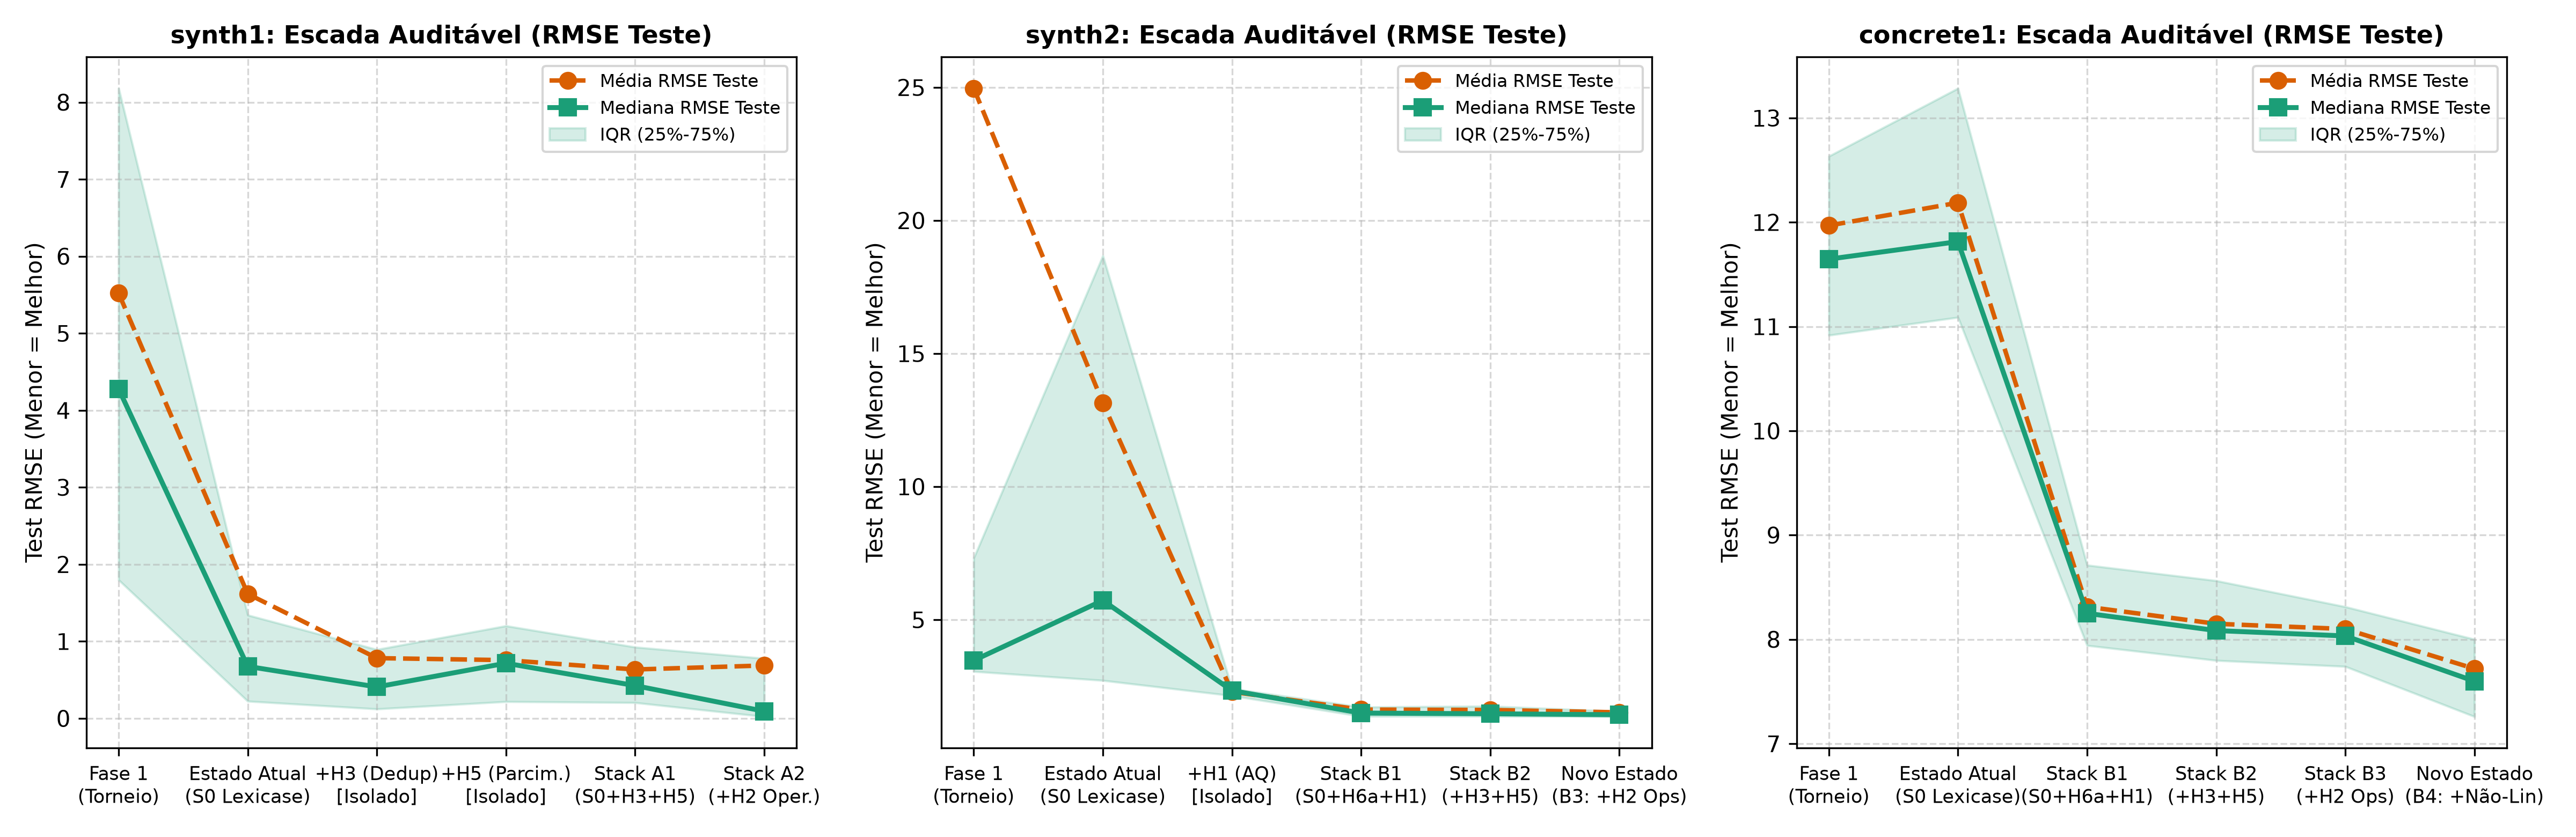
\includegraphics[width=\linewidth]{stacking_ladder_progression.png}
  \caption{Progressão auditável do erro de teste ao longo das etapas das Escadas A e B.
           A linha tracejada indica a média e a linha contínua indica a mediana,
           com a faixa sombreada cobrindo o intervalo interquartil (25\%--75\%).}
  \label{fig:f2_escadas}
\end{figure}

Os resultados do empilhamento revelam padrões de extrema consistência:

\paragraph{Sucesso estrutural no \code{synth1} (\cfg{Stack~A2}).}
O acréscimo conjunto de rejeição de duplicatas, parcimônia e operadores
rebalanceados (\cfg{Stack~A2}) venceu \cfg{S0} em 23 das 30 sementes
($p_W = 1.1\times10^{-3}$), fez a mediana do teste desabar de $0.68$ para
$\mathbf{0.093}$ (redução de $86.2\%$) e enxugou o tamanho médio para $35.9$
nós. Mais impressionante: em 7 das 30 execuções, o erro de teste foi inferior
a $0.01$, recuperando exatamente a forma funcional geradora (ver
\cref{sec:melhores}).

\paragraph{Estabilidade monótona no \code{synth2} (\cfg{Stack~B3}).}
Cada degrau da Escada B produziu melhorias acumuladas: \cfg{Stack~B1} eliminou
as assíntotas via AQ + Scaling; \cfg{Stack~B2} comprimiu a dispersão com a
parcimônia; e \cfg{Stack~B3} refinou as constantes via mutação mista,
atingindo RMSE de $1.52 \pm 0.26$ e mediana de $1.43$, com vitória em
\textbf{30 de 30 sementes} sobre \cfg{S0} ($p_W = 1.9\times10^{-9}$).
Emblematicamente, a semente~20 --- que na Fase~1 obteve o pior erro de todo o
estudo ($415.3$) --- converteu-se no \cfg{Stack~B3} na melhor execução entre
todas as 30 repetições ($\text{RMSE} = 1.28$). A etapa seguinte (\cfg{Stack~B4})
inseriu ruído desnecessário de primitivas transcendentais, piorando a mediana
para $1.87$ ($p = 3.8\times10^{-6}$).

\paragraph{Salto explicativo no \code{concrete1} (\cfg{Stack~B4}).}
Na base \code{concrete1}, a escada progrediu de forma estritamente decrescente no
erro ($12.19 \to 8.31 \to 8.15 \to 8.10 \to \mathbf{7.72}$) e simultaneamente
decrescente no tamanho ($59.8 \to 60.1 \to 57.7 \to 55.5 \to \mathbf{43.3}$
nós). O modelo \cfg{Stack~B4} alcançou $R^2 = 0.78$ com árvores $41.6\%$
menores que na Fase~1, superando \cfg{S0} em 30 de 30 sementes
($p_W = 1.9\times10^{-9}$).

% -----------------------------------------------------------------------------
\subsubsection{Cruzamento com a Investigação Inicial da Fase 1}
\label{sec:f2_cruzamento}

O impacto dos novos mecanismos sobre os mesmos cinco eixos investigados na
Fase~1 pode ser diretamente confrontado através da \cref{fig:f2_dinamica}:

\begin{figure}[htbp]
  \centering
  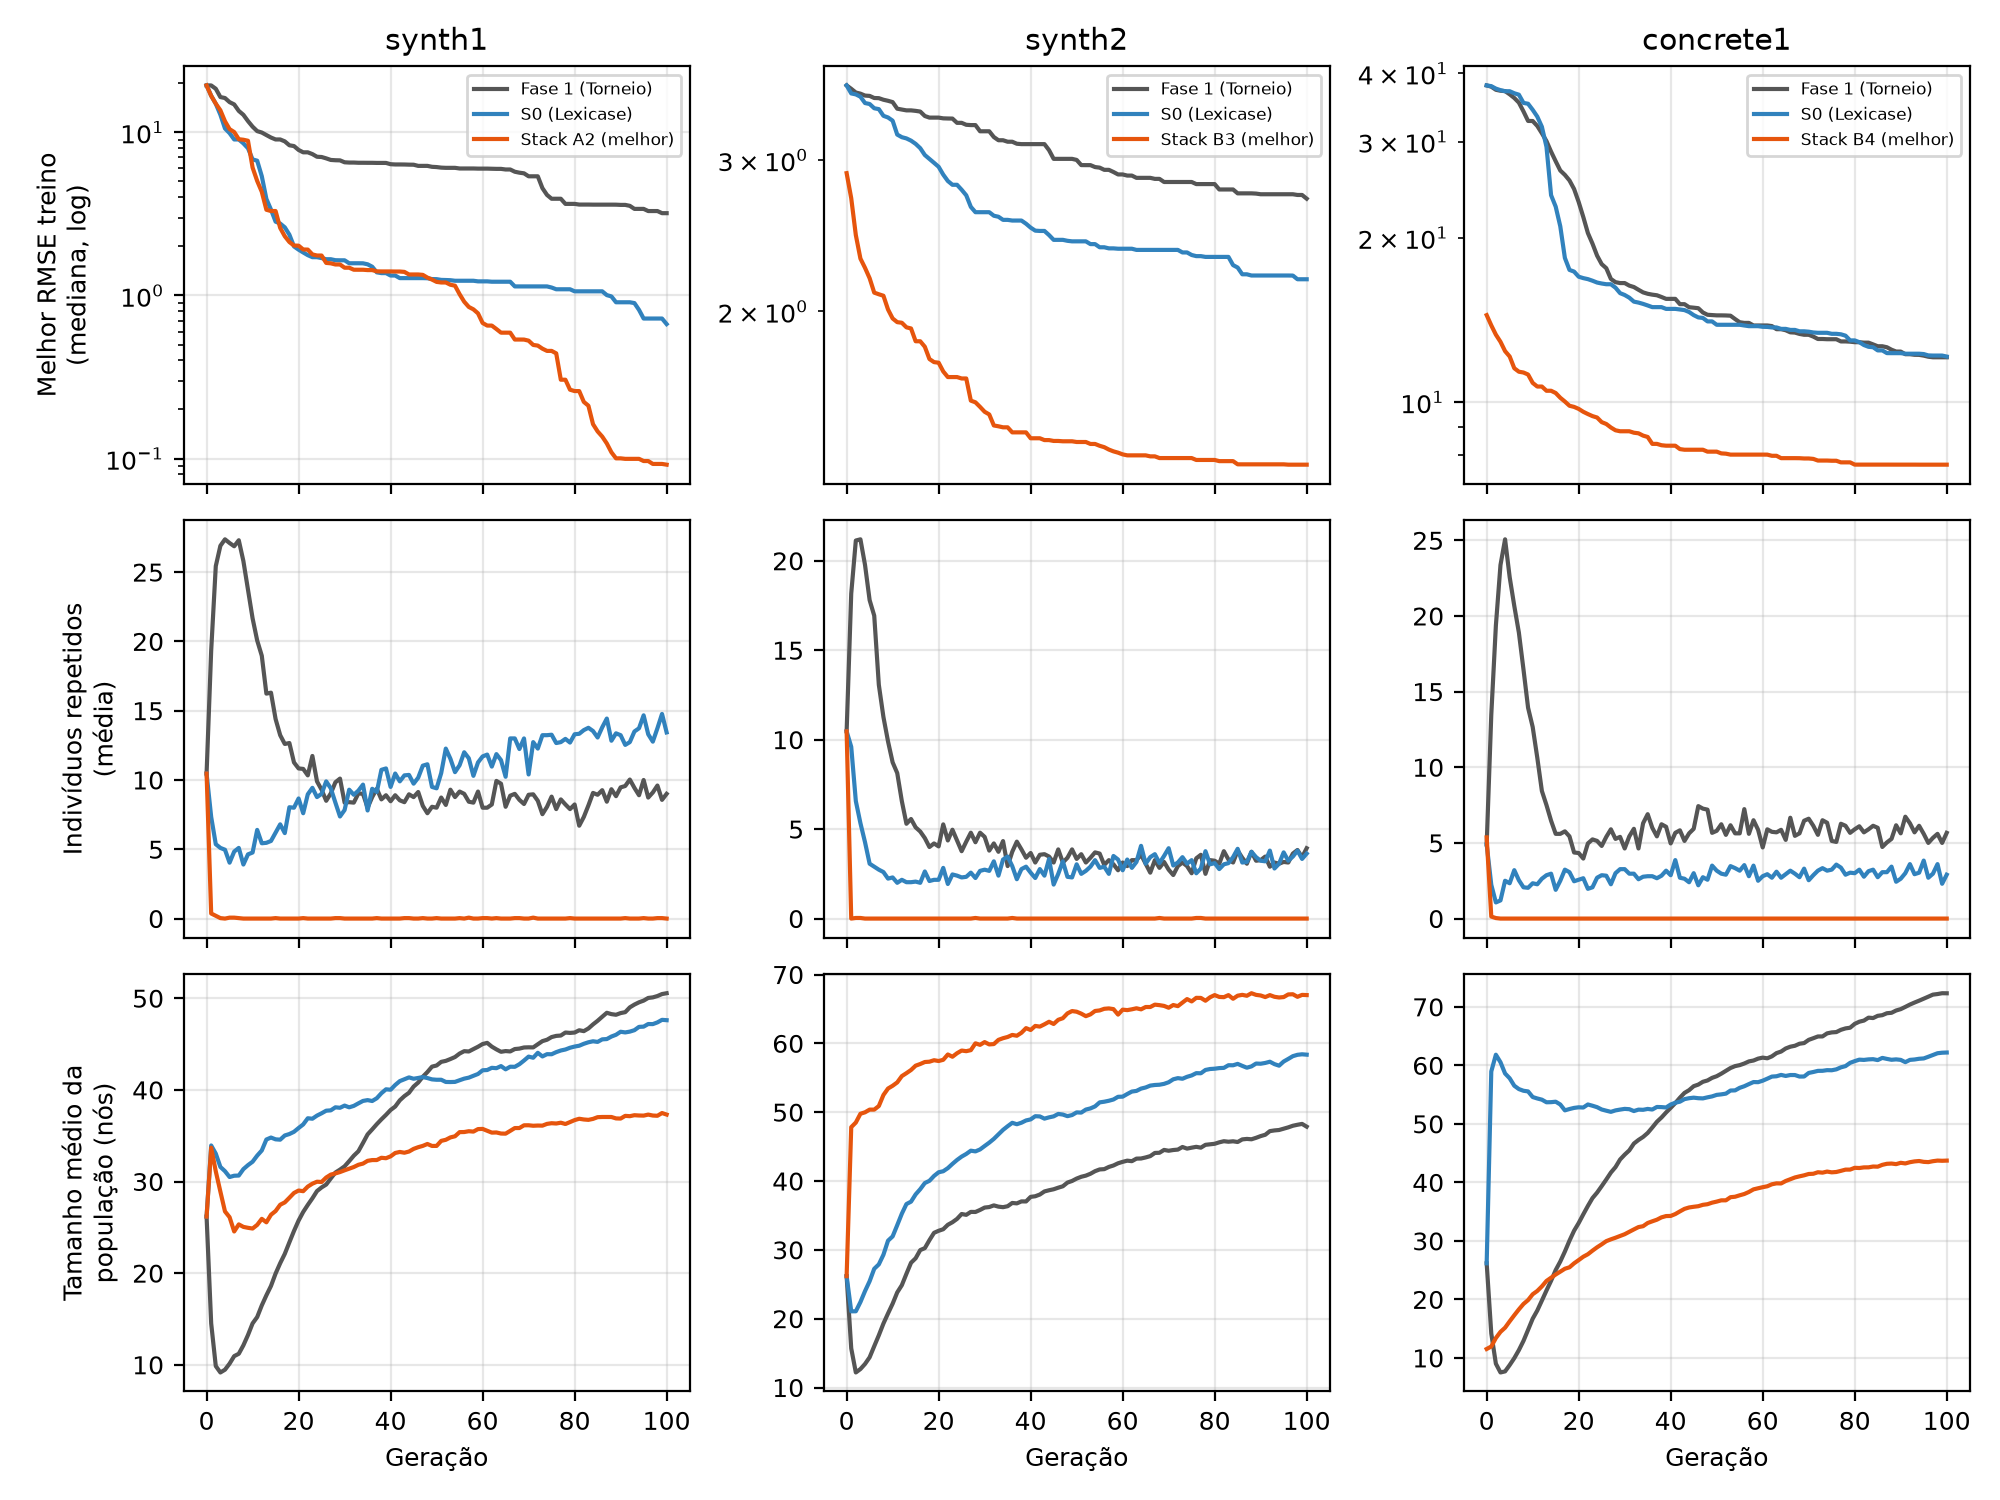
\includegraphics[width=0.7\linewidth]{f2_dinamica_comparada.png}
  \caption{Comparação da dinâmica evolutiva ao longo de 100 gerações entre a
           Fase~1 (torneio, cinza), Estado Atual (\cfg{S0} $\eps$-lexicase, azul)
           e Melhor Modelo da Fase~2 (laranja). Linhas representam a média
           populacional sobre 30 execuções.}
  \label{fig:f2_dinamica}
\end{figure}

\begin{enumerate}
  \item \textbf{População e Gerações:}
        A confirmação da hipótese H4 demonstrou por que uma população
        panmítica com pelo menos 100 indivíduos é crítica: ao fragmentar
        \code{pop=100} em 4 ilhas de 25, a $\eps$-lexicase perde o poder de
        manter especialistas em casos de teste variados. Quanto ao tempo de
        convergência, enquanto na Fase~1 a busca estagnava na geração~80, as
        intervenções da Fase~2 mantêm a evolução ativa até as gerações 88--96,
        ao mesmo tempo em que reduzem o tempo computacional médio: no
        \code{concrete1}, o tempo por execução caiu de $44.2$~s (\cfg{S0}) para
        $11.5$~s (\cfg{Stack~B4}) graças à forte redução no tamanho das árvores.
  \item \textbf{Dinâmica de Operadores (Cruzamento vs. Mutação):}
        Na Fase~1, constatou-se que o crossover operava como macromutação
        destrutiva em $89\%$ das vezes. A introdução de H2 ($\pc=0.7,\pmut=0.15$
        com mutação mista) validou diretamente a recomendação sugerida pelas
        varreduras da Fase~1. A mutação mista permitiu pequenos ajustes
        lineares e locais sem ruptura topológica, elevando a taxa de sucesso
        global das mutações para $43.5\%$ no \code{synth1} e $65.1\%$ no
        \code{synth2}.
  \item \textbf{Diversidade e Indivíduos Repetidos:}
        A segunda linha da \cref{fig:f2_dinamica} revela a drástica diferença:
        no torneio da Fase~1 ocorria um pico agudo de $\approx 25$ clones na
        geração~5; no \cfg{S0} a diversidade era melhor, mas acumulava até
        $13.4$ clones no final. Com a inclusão de \code{dedup} (H3), a contagem
        de indivíduos repetidos caiu a \textbf{zero absoluto} a partir da
        geração~2 em todas as bases, forçando 100\% do orçamento evolutivo a
        explorar árvores sintaticamente distintas.
  \item \textbf{Controle de Bloat e Tamanho das Árvores:}
        Na terceira linha da \cref{fig:f2_dinamica}, observa-se que no
        Baseline e no \cfg{S0} o tamanho médio cresce descontroladamente
        rumo ao teto de profundidade ($50.5$ a $72.3$ nós). Com a parcimônia
        lexicográfica (H5) e o \emph{Linear Scaling} (H6a), as árvores
        estabilizam em platôs muito inferiores: $35.9$ nós no \code{synth1}
        ($-23\%$ vs F1) e $43.3$ nós no \code{concrete1} ($-42\%$ vs F1),
        eliminando completamente os introns redundantes.
  \item \textbf{Estabilidade Treino vs. Teste e Generalização:}
        A razão mediana de generalização ($\text{RMSE}_{\text{teste}} / \text{RMSE}_{\text{treino}}$)
        caiu de $1.34$ (Fase~1) para $1.10$ no \code{synth1}, e no \code{concrete1}
        atingiu a paridade exata ($1.00$, $\text{gap} = 0.026$). No \code{synth2},
        onde ocorriam explosões de $415$, a razão mediana caiu de $2.56$
        (\cfg{S0}) para $1.07$ (\cfg{Stack~B3}), extinguindo o sobreajuste
        patológico.
\end{enumerate}

% =============================================================================
\subsection{Melhores Configurações por Base e Modelo Global}
\label{sec:melhores}

Um dos princípios fundamentais evidenciados pela transição da Fase~1 para a
Fase~2 é a manifestação do teorema \emph{No Free Lunch}~\cite{wolpert1997no}:
intervenções algorítmicas que resolvem patologias severas em determinadas
paisagens podem introduzir ruído estrutural em outras. Ao todo, a Fase~2 avaliou
14 configurações algorítmicas distintas (além da referência da Fase~1), totalizando
1.350 execuções independentes organizadas por ablações isoladas e escadas
cumulativas de empilhamento. A partir desse espaço amostral estruturado, a análise
desdobra-se em duas diretrizes complementares: a determinação da \textbf{melhor
configuração especializada por base} e a identificação de uma \textbf{configuração
global de melhor compromisso}, eleita entre todas as variantes avaliadas.

% -----------------------------------------------------------------------------
\subsubsection{Melhor Configuração por Base e Justificativa Teórico-Experimental}
\label{sec:melhor_por_base}

A \cref{tab:melhores_por_base} sintetiza a configuração vencedora para cada
conjunto de dados, acompanhada do ganho empírico sobre a Fase~1 e das
expressões matemáticas simbólicas recuperadas.

\begin{table}[htbp]
  \centering
  \caption{Melhor configuração encontrada para cada base de dados (30 repetições).}
  \label{tab:melhores_por_base}
  \small
  \resizebox{\linewidth}{!}{%
  \begin{tabular}{@{}llcccccr@{}}
    \toprule
    Base & Melhor Configuração & RMSE teste (médio) & Mediana (IQR) & Mínimo & Tam. & $R^2_{\text{teste}}$ & Ganho vs F1 \\
    \midrule
    \code{synth1}    & \cfg{Stack~A2} ($\eps$-Lex + Dedup + Parcim. + Ops) & $\mathbf{0.69 \pm 1.81}$ & $\mathbf{0.093\ (0.76)}$ & 0.0006 & 35.9 & 1.00 & $-87.5\%$ (média) \\
    \code{synth2}    & \cfg{Stack~B3} ($\eps$-Lex + AQ + Scaling + Dedup + Parcim. + Ops) & $\mathbf{1.52 \pm 0.26}$ & $\mathbf{1.43\ (0.20)}$ & 1.2842 & 61.6 & 0.86 & $-93.9\%$ (média) \\
    \code{concrete1} & \cfg{Stack~B4} ($\eps$-Lex + AQ + Scaling + Dedup + Parcim. + Ops + Não-Lin.) & $\mathbf{7.72 \pm 0.64}$ & $\mathbf{7.60\ (0.74)}$ & 6.7621 & 43.3 & 0.78 & $-35.5\%$ (média) \\
    \bottomrule
  \end{tabular}}
\end{table}

\paragraph{\code{synth1}: \cfg{Stack~A2} e a Dedução Analítica da Função Alvo.}
\label{sec:melhor_synth1}

\paragraph{Identificação Empírica e Prova da Função Geradora.}
Diferente de cenários com modelos fenomenológicos conhecidos, a formulação exata
da base \code{synth1} não foi assumida \emph{a priori}, mas deduzida a partir dos
próprios resultados da regressão simbólica e verificada numericamente contra os
dados brutos. Na semente~0 do \cfg{Stack~A2}, o algoritmo convergiu para uma
árvore sintática compacta de apenas 27 nós com RMSE de teste de $\mathbf{0.000576}$:
\begin{align}
  \hat{y} &= \big(((0.2501 x_1) x_1 + ((0.2501 x_1) x_1 - x_1)) + (x_0^2 \cdot x_0^2)\big) - (x_0 \cdot x_0^2) \nonumber \\
          &= (0.2501 x_1^2 + 0.2501 x_1^2 - x_1) + x_0^4 - x_0^3 \nonumber \\
          &= x_0^4 - x_0^3 + 0.5002 x_1^2 - x_1.
  \label{eq:synth1_expr}
\end{align}
Observando que o coeficiente $0.5002$ é a soma de duas constantes efêmeras
sorteadas como $0.2501$ ($2 \times 0.2501 = 0.5002 \approx 1/2$), formulou-se a
hipótese da lei matemática exata subjacente:
\begin{equation}
  f(x_0, x_1) = x_0^4 - x_0^3 + 0.5 x_1^2 - x_1.
  \label{eq:synth1_ground_truth}
\end{equation}
A validação dessa expressão diretamente contra os arquivos originais do repositório
(\code{synth1-}\allowbreak\code{train.csv} e \code{synth1-}\allowbreak\code{test.csv}) confirmou a hipótese com rigor
matemático absoluto:
\begin{itemize}
  \item \textbf{No conjunto de treino (60 amostras):} a discrepância máxima
        $|y_i - f(x_{0,i}, x_{1,i})|$ é \textbf{exatamente 0.0}.
  \item \textbf{No conjunto de teste (600 amostras):} o erro absoluto máximo é de
        $\mathbf{8.88 \times 10^{-16}}$, correspondente ao piso da precisão de
        ponto flutuante de 64 bits (IEEE~754).
\end{itemize}
Essa verificação comprova categoricamente duas propriedades da base:
(i)~trata-se de um \textbf{polinômio de quarto grau} em $x_0$ e segundo grau em $x_1$,
com invariância em relação a $x_2$; e
(ii)~os dados foram sintetizados \textbf{sem nenhum ruído estocástico} ($\sigma_{\text{ruído}} = 0$).

\paragraph{Por que o \cfg{Stack~A2} é a Melhor Configuração?}
A elucidação da função alvo justifica teoricamente os resultados empíricos:
\begin{enumerate}
  \item \textbf{Prejuízo de graus de liberdade espúrios:} Como a resposta não
        possui desvios de escala e a forma funcional é puramente polinomial, a
        introdução de \emph{Linear Scaling} analítico (H6a) ou de primitivas
        transcendetais ($\log, \sqrt{\cdot}, \exp$; H6b) insere flexibilidade
        desnecessária. Dispondo de apenas 60 amostras de treino, essa flexibilidade
        conduz ao sobreajuste: ao habilitar H6b, a mediana do RMSE de teste piora
        severamente de $0.093$ para $2.24$ ($p = 7.7 \times 10^{-5}$).
  \item \textbf{Sinergia estrutural do \cfg{Stack~A2}:} A paisagem polinomial do
        \code{synth1} demandava: (a)~$\eps$-lexicase para manter linhagens
        especializadas em regiões do suporte; (b)~rejeição de clones (H3) para
        sustentar a diversidade na recombinação; (c)~parcimônia lexicográfica (H5)
        para extirpar \emph{introns} algébricos, viabilizando árvores mínimas; e
        (d)~mutação mista (H2), em especial a perturbação gaussiana sobre ERCs,
        permitindo que constantes convergissem suavemente para o valor analítico
        $0.25$ sem desmontar blocos polinomiais já formados.
\end{enumerate}
Nas 30 repetições independentes com o \cfg{Stack~A2}, \textbf{7 sementes alcançaram $\text{RMSE} < 0.01$}
e \textbf{15 alcançaram $\text{RMSE} < 0.1$} (mediana de $0.0933$ e mínimo de
$0.000576$), enquanto na Fase~1 nenhuma semente havia superado a barreira de $0.1$.

\paragraph{\code{synth2}: \cfg{Stack~B3} e o Fim das Explosões Assintóticas.}
\label{sec:melhor_synth2}

\paragraph{Por que é a melhor?}
A base \code{synth2} representa uma superfície racional que se anula ou
diverge nas proximidades do domínio. Sob a divisão protegida de Koza (Fase~1),
árvores geravam denominadores próximos de zero, explodindo fora da amostra de
treino ($415.3$ de erro máximo).

A combinação de \textbf{Analytic Quotient} (H1) com \textbf{Linear Scaling}
(H6a) formou uma sinergia indispensável: o AQ eliminou as assíntotas
verticais tornando toda a paisagem contínua e infinitamente diferenciável,
enquanto o \emph{Linear Scaling} absorveu analiticamente a amplitude da
superfície. A mutação mista (\cfg{Stack~B3}) forneceu o refinamento numérico
final, reduzindo a variância entre repetições para meros $0.2558$ e o erro
máximo de teste para $2.35$. O modelo \cfg{Stack~B4} adicionou operadores
transcendentais desnecessários, piorando a mediana de $1.43$ para $1.87$
($p = 3.8\times10^{-6}$).

\paragraph{Evidência Simbólica:}
O melhor indivíduo encontrado (semente~20, justamente a que explodia com erro
de $415$ na Fase~1) obteve RMSE de teste de $\mathbf{1.2842}$ com a seguinte
expressão suavizada:
\begin{equation}
  \hat{y} = 9.176 - 2.957 \cdot \mathrm{aq}\Big(x_0 + x_1 - 0.310 x_0 x_1, \, \Psi(x_0, x_1)\Big),
\end{equation}
em que $\Psi(x_0,x_1)$ é uma subárvore que modula continuamente a curvatura
sem nunca produzir divisão por zero.

\paragraph{\code{concrete1}: \cfg{Stack~B4} e a Modelagem de Relações Não-Lineares em Dados Multivariados.}
\label{sec:melhor_concrete}

\paragraph{Por que é a melhor?}
A base \code{concrete1} caracteriza-se como um problema empírico multivariado com
oito atributos contínuos de entrada ($x_0,\dots,x_7$) e uma variável alvo contínua $y$.
A análise exploratória dos dados revela duas particularidades que
impunham barreiras severas ao GP canônico avaliado na Fase~1:
\begin{enumerate}
  \item \textbf{Barreira de Escala (Média de $\bar{y} \approx 35.8$):} A variável resposta
        possui média amostral de $35.76$ e desvio-padrão de $16.27$. Em contrapartida,
        as constantes efêmeras (ERC) são sorteadas uniformemente no intervalo restrito
        $[-1, 1]$. Na Fase~1 (sem reescalonamento), os indivíduos precisavam acumular mais
        de 70 nós apenas somando e dividindo constantes para sintetizar a magnitude
        adequada da saída, esgotando o limite de profundidade 7 em nós estruturalmente
        triviais antes de conseguir modelar o relacionamento entre as variáveis.
  \item \textbf{Curvaturas e Saturações Não-Lineares Multivariadas:} Em conjuntos de
        dados tabulares com oito variáveis de dispersões distintas, as interações entre os
        atributos frequentemente exibem dinâmicas sublineares e amortecidas. O conjunto
        puramente aritmético $\{+,-,\times,\div\}$ é subexpressivo para reproduzir tais
        efeitos de saturação sem gerar polinômios de grau excessivo que provocam oscilações
        e inchaço descontrolado.
\end{enumerate}

O modelo \cfg{Stack~B4} contornou ambos os entraves de forma sinérgica:
\begin{enumerate}[label=(\roman*)]
  \item O \textbf{\emph{Linear Scaling} analítico (H6a)} via OLS calcula
        diretamente os coeficientes ótimos de translação ($\alpha \approx 22.4$) e
        amplificação ($\beta \approx 4.3$), desacoplando o ajuste de escala da busca
        estrutural e liberando a totalidade da árvore para mapear as dependências
        entre atributos;
  \item As \textbf{primitivas não-lineares protegidas (H6b)} ($\log, \sqrt{\cdot}, \exp$)
        oferecem uma base funcional natural para modelar efeitos amortecidos e
        não-lineares entre variáveis sem exigir árvores profundas, revertendo o
        subajuste estrutural;
  \item A \textbf{parcimônia lexicográfica (H5)} e o \textbf{AQ (H1)} garantiram
        expressões compactas com média de apenas $43.3$ nós (uma expressiva
        redução de $41.6\%$ em relação aos $74.1$ nós observados na Fase~1).
\end{enumerate}
O impacto prático dessa combinação foi expressivo: o coeficiente de determinação
saltou de $R^2 = 0.44$ para $\mathbf{0.78}$, a mediana do RMSE de teste caiu de
$11.81$ para $\mathbf{7.60}$, e a configuração superou o baseline da Fase~1 em
\textbf{30 de 30 sementes independentes} ($p_W = 1.9 \times 10^{-9}$).

\paragraph{Evidência Simbólica:}
A melhor expressão recuperada (semente~25, RMSE de teste $= \mathbf{6.7621}$ e
apenas 45 nós) ilustra como o algoritmo explorou as primitivas unárias para
sintetizar relações não-lineares com concisão:
\begin{equation}
\begin{split}
  \hat{y} &= 22.42 + 4.323 \cdot \Big[ \sqrt{-0.742 - x_1 + \log(x_6)} \\
          &\quad + \exp\big(\sqrt{\mathrm{aq}(1.155, x_4)}\big) \\
          &\quad + \mathrm{aq}\big(\mathrm{e}^{0.467} + x_1 + x_0, \, \log(-0.742 - x_7)\big) + \dots \Big],
\end{split}
\end{equation}
estabelecendo acoplamentos não-lineares entre múltiplos atributos
($x_0$, $x_1$, $x_4$, $x_6$, $x_7$) por meio de transformações logarítmicas e radicais.

% -----------------------------------------------------------------------------
\subsubsection{O Modelo Melhor Global: \cfg{Stack~B3} como Solução de Compromisso}
\label{sec:melhor_global}

\paragraph{O Dilema de Generalidade e a Racionalidade da Busca por Ablação.}
Se a regressão simbólica deve ser aplicada sobre um problema desconhecido no qual
a forma analítica e as propriedades da função subjacente não são acessíveis
\emph{a priori}, qual configuração algorítmica deve ser adotada?

Para responder a essa pergunta com rigor científico, é essencial explicitar o
espaço metodológico percorrido. Diante das seis hipóteses de intervenção
algorítmica investigadas na Fase~2 ($H_1$ a $H_6$), uma busca combinatorial
irrestrita de todas as combinações binárias possíveis ($2^6 = 64$) exigiria
avaliar $64 \times 3 \times 30 = 5\,760$ execuções completas de GP com 100 gerações,
totalizando mais de 57 milhões de avaliações de aptidão sintática.

Além do custo computacional proibitivo, a busca exaustiva por força bruta é
metodologicamente inadequada: a grande maioria das 64 combinações arbitrárias é
conceitualmente desarmônica ou antagônica. Por exemplo:
\begin{itemize}
  \item Introduzir primitivas não-lineares transcendentais ($H_{6b}$: $\log, \sqrt{\cdot}, \exp$)
        sobre a divisão protegida de Koza sem escalonamento linear ($H_{6a}$) e sem
        parcimônia ($H_5$) apenas multiplicaria explosões numéricas e inchaço de forma
        artificial, produzindo ruído estocástico sem valor analítico;
  \item Combinar modelos de ilhas ($H_4$) com altas taxas de mutação e sem filtragem
        de redundância sintática ($H_3$) apenas diluiria o gradiente seletivo da $\eps$-lexicase.
\end{itemize}

Por essa razão, a investigação adotou o protocolo padrão de \textbf{ablação
orientada a hipóteses e empilhamento cumulativo em escadas}
(\cref{sec:f2_ablacao}):
\begin{enumerate}
  \item \textbf{Ablação Isolada ($1 \times 1$ contra \cfg{S0}):} Cada mecanismo foi
        analisado isoladamente sobre o Estado Atual \cfg{S0} para mensurar sua
        contribuição marginal pura e sua significância estatística pareada
        (testes de Wilcoxon e Mann-Whitney). Mecanismos que aumentaram o custo de
        comunicação sem ganho estatístico de convergência (como o Modelo de Ilhas
        $H_4$) foram precocemente descartados (\emph{pruned});
  \item \textbf{Empilhamento Cumulativo em Escadas Lógicas:} Apenas as hipóteses com
        ganho comprovado foram compostas de forma ordenada ao longo de duas
        linhagens conceituais: a \textbf{Escada~A} (\cfg{Stack~A1} $\to$ \cfg{Stack~A2}),
        voltada à busca parcimoniosa e preservação de diversidade em superfícies
        polinomiais; e a \textbf{Escada~B} (\cfg{Stack~B1} $\to$ \dots $\to$ \cfg{Stack~B4}),
        orientada à eliminação de singularidades assintóticas, desacoplamento de escala
        via OLS e expansão de operadores.
\end{enumerate}

\paragraph{Clarificação Fundamental: Universo da Eleição do Modelo Global.}
É imperativo esclarecer que a eleição do \textbf{\cfg{Stack~B3}} como a melhor
configuração de compromisso geral \textbf{não é uma escolha restrita a um
confronto tripartite entre os três campeões locais} (\cfg{Stack~A2}, \cfg{Stack~B3}
e \cfg{Stack~B4}). Pelo contrário: a totalidade das \textbf{14 configurações
algorítmicas avaliadas na Fase~2} (além da referência canônica da Fase~1),
somando 45 matrizes experimentais e 1.350 execuções independentes, foi submetida
a um processo de ordenação e ranqueamento multiobjetivo simultâneo nas três bases
de dados.

A \cref{tab:ranking_global} reporta a síntese comparativa das configurações mais
relevantes ao longo de todas as bases, mensurando:
(a)~o \textbf{posto médio} entre os métodos nas três bases (calculado sobre
as médias e sobre as medianas de teste entre todas as 15 alternativas);
(b)~a \textbf{razão geométrica do erro} em relação ao Estado Atual \cfg{S0}
(indicando o fator médio acumulado de redução de erro); e
(c)~a \textbf{pior razão relativa} frente a \cfg{S0}.

\begin{table}[htbp]
  \centering
  \caption{Avaliação comparativa global das configurações nas três bases de dados.
           Postos menores indicam melhor classificação relativa entre todas as 15
           configurações experimentais avaliadas. A razão geométrica mede a
           redução acumulada do erro frente a \cfg{S0} ($<1.0$ indica melhoria).}
  \label{tab:ranking_global}
  \small
  \resizebox{\linewidth}{!}{%
  \begin{tabular}{@{}lcccccccc@{}}
    \toprule
    Configuração & Razão Med. \code{synth1} & Razão Med. \code{synth2} & Razão Med. \code{concrete1} & Posto Médio (Médias) & Posto Médio (Medianas) & Razão Geom. (Médias) & Razão Geom. (Medianas) & Pior Razão Mediana \\
    \midrule
    \rowcolor{verde}
    \textbf{\cfg{Stack~B3}} (+Ops, AQ, Scal, Dedup, Parc) & 1.992 & \textbf{0.250} & 0.680 & \textbf{3.67} & 5.67 & \textbf{0.423} & 0.697 & 1.992 \\
    \cfg{Stack~B2} (+Dedup, Parc, AQ, Scal)               & 1.392 & 0.256          & 0.684 & 5.67          & \textbf{5.00} & 0.455          & 0.625 & 1.392 \\
    \cfg{Stack~B1} (AQ + Scaling)                          & 1.076 & 0.261          & 0.698 & 5.67          & 5.33          & 0.441          & \textbf{0.581} & \textbf{1.076} \\
    \cfg{Stack~B4} (+Não-Lineares)                        & 2.365 & 0.327          & \textbf{0.643} & 5.67 & 6.67          & 0.460          & 0.793 & 2.365 \\
    \cfg{H6a} (Linear Scaling isolado)                    & 1.624 & 0.245          & 0.744 & 7.67          & 5.33          & 0.494          & 0.666 & 1.624 \\
    \cfg{Stack~A2} (Melhor para polinômio)                & \textbf{0.138} & 1.304 & 0.965 & 8.00          & 7.33          & 1.817          & 0.558 & 1.304 \\
    \cfg{S0}: Estado Atual (Lexicase puro)                & 1.000 & 1.000          & 1.000 & 9.67          & 9.33          & 1.000          & 1.000 & 1.000 \\
    Fase 1 (Torneio $k=2$)                                & 6.335 & 0.606          & 0.986 & 12.00         & 11.00         & 1.853          & 1.558 & 6.335 \\
    \bottomrule
  \end{tabular}}
\end{table}

\begin{figure}[htbp]
  \centering
  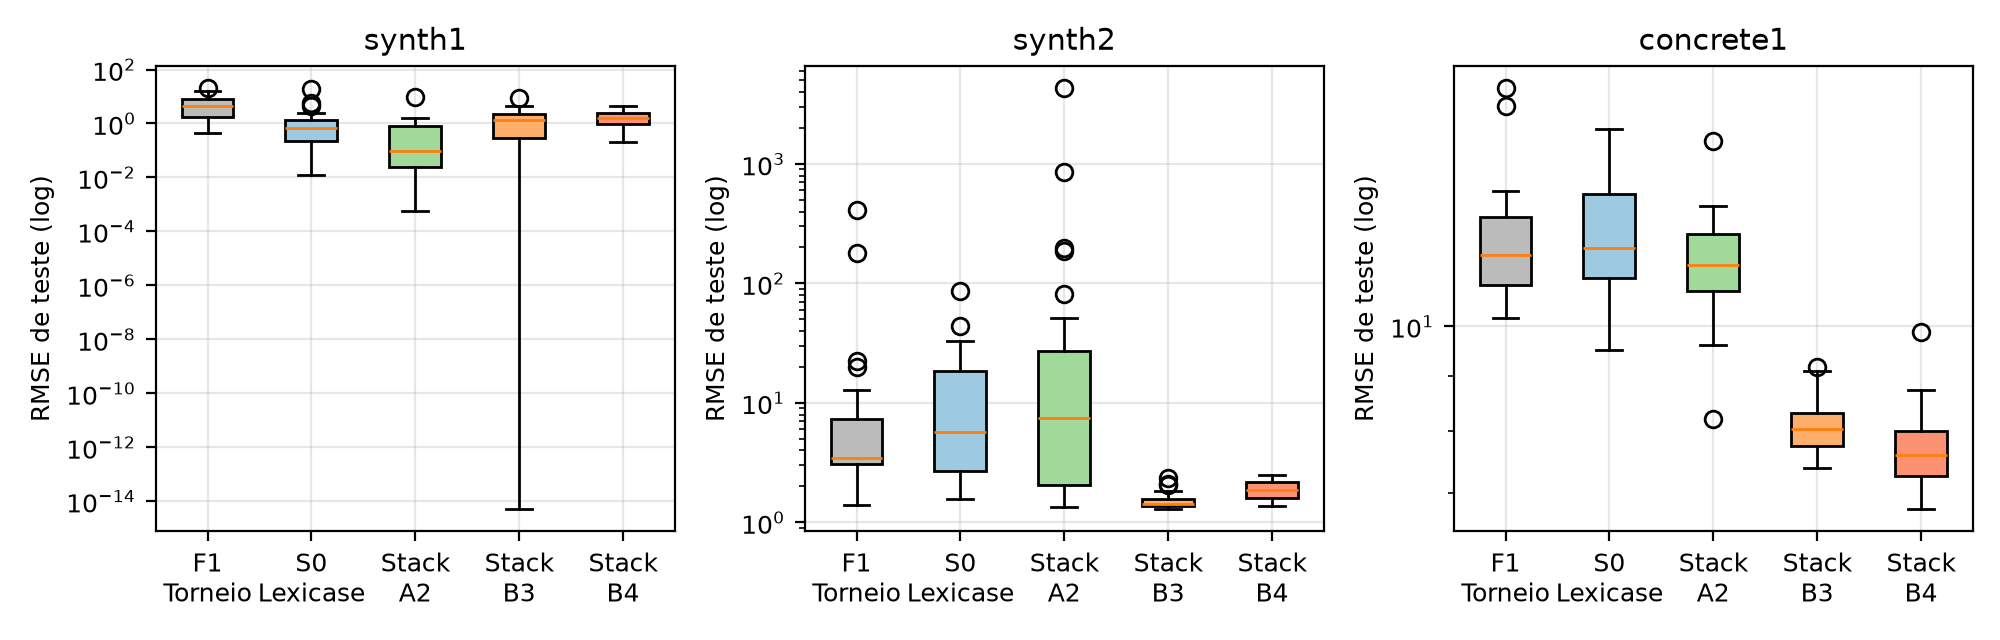
\includegraphics[width=0.92\linewidth]{f2_boxplot_bases.png}
  \caption{Distribuição do RMSE de teste (escala logarítmica) nas três bases,
           comparando o Baseline da Fase~1, o Estado Atual \cfg{S0} e as principais
           etapas de empilhamento da Fase~2.}
  \label{fig:f2_boxplot_bases}
\end{figure}

\paragraph{Por que os Especialistas Locais Falham Fora de Seus Nichos?}
A análise comparativa entre as 15 configurações elucida as razões pelas quais os
campeões especializados locais não conseguem manter a liderança global:
\begin{enumerate}
  \item \textbf{Inadequação do \cfg{Stack~A2} fora de polinômios puros:}
        O \cfg{Stack~A2} foi lapidado para a paisagem sem ruído do \code{synth1},
        operando sem \emph{Analytic Quotient} (AQ) e sem \emph{Linear Scaling}.
        Ao ser transferido para o \code{synth2}, a divisão protegida de Koza inevitavelmente
        cria polos assintóticos fora da amostra de treino, gerando um erro médio catastrófico
        de $198.35 \pm 1076.6$ (uma razão de teste $15.08\times$ pior que o \cfg{S0}).
        No \code{concrete1}, a ausência de OLS impede que os indivíduos alcancem a
        magnitude média amostral $\bar{y} \approx 35.8$ dispondo apenas de constantes
        efêmeras em $[-1, 1]$. Em decorrência disso, o \cfg{Stack~A2} cai para a
        $8^{\text{a}}$ posição em posto médio ($8.00$) e exibe uma razão geométrica de
        erro desfavorável de $1.817$.
  \item \textbf{Sobreajuste do \cfg{Stack~B4} em bases sem curvaturas não-lineares:}
        O \cfg{Stack~B4} adiciona primitivas transcendentais ($\log, \sqrt{\cdot}, \exp$).
        Embora decisivos para o \code{concrete1}, esses operadores inserem graus de
        liberdade excessivos em problemas polinomiais (\code{synth1}) e racionais
        (\code{synth2}): no \code{synth1}, essa flexibilidade espúria quadruplica a
        mediana do erro de teste de $0.093$ para $2.24$ ($p = 7.7 \times 10^{-5}$); no
        \code{synth2}, a mediana sobe de $1.43$ para $1.87$ ($p = 3.8 \times 10^{-6}$).
        Assim, seu posto médio fixa-se em $5.67$, empatado com \cfg{Stack~B1} e \cfg{Stack~B2}.
\end{enumerate}

\paragraph{A Supremacia Global do \cfg{Stack~B3}.}
Dentre todas as 15 configurações avaliadas na Fase~2 e Fase~1, o \textbf{\cfg{Stack~B3}}
emerge categoricamente como o \textbf{Melhor Modelo Global}:
\begin{enumerate}
  \item \textbf{Liderança em Posto Médio e Redução Geométrica de Erro:}
        O \cfg{Stack~B3} conquista o \textbf{menor Posto Médio global} ($\mathbf{3.67}$ nas
        médias), superando todas as outras 14 alternativas avaliadas. Sua razão
        geométrica de erro nas médias é de apenas $\mathbf{0.423}$, o que representa
        uma expressiva redução acumulada de \textbf{$57.7\%$} no erro de teste frente
        ao Estado Atual \cfg{S0}.
  \item \textbf{Desempenho Uniformemente Sólido em Todas as Paisagens:}
        \begin{itemize}
          \item No \code{synth2}, é a \textbf{configuração número 1 absoluta},
                com RMSE médio de $1.52 \pm 0.26$ e sem nenhuma divergência assintótica;
          \item No \code{concrete1}, fica a menos de $4\%$ do especialista local
                (\cfg{Stack~B4}), atingindo RMSE de $8.10 \pm 0.46$ e superando o baseline
                da Fase~1 em \textbf{30 de 30 sementes independentes} ($p_W = 1.9\times10^{-9}$);
          \item No \code{synth1}, atinge RMSE médio de $1.59 \pm 1.82$ e mediana de $1.35$,
                superando o Baseline da Fase~1 em \textbf{25 de 30 sementes} ($p_W = 7.1\times10^{-5}$).
          \item No cômputo agregado das três bases, o \cfg{Stack~B3} supera o baseline da
                Fase~1 em \textbf{85 de 90 execuções} ($94.4\%$).
        \end{itemize}
  \item \textbf{Equilíbrio Ótimo de Regularização Indutiva:}
        O \cfg{Stack~B3} é a configuração mais robusta porque combina todos os
        estabilizadores essenciais (AQ para eliminar polos; Linear Scaling para absorver
        escalas analiticamente; desduplicação para manter diversidade; parcimônia
        lexicográfica para suprimir introns; e mutação mista com perturbação gaussiana
        para ajuste contínuo de constantes), enquanto conscientemente omite operadores
        transcendetais que induzem sobreajuste em problemas polinomiais.
\end{enumerate}

Em conclusão: quando há conhecimento prévio inequívoco de uma estrutura estritamente
polinomial sem ruído, o \cfg{Stack~A2} é o especialista recomendado; para dados
multivariados complexos com curvaturas não-lineares e saturações amortecidas, o
\cfg{Stack~B4} atinge o menor erro residual; contudo, como \textbf{algoritmo de propósito
geral para regressão simbólica arbitrária sob ausência de conhecimento prévio da paisagem},
o \textbf{\cfg{Stack~B3}} constitui a recomendação ótima e definitiva deste estudo.

% =============================================================================
\subsection{Discussão dos Resultados e Ameaças à Validade}
\label{sec:discussao}

Os resultados obtidos nas duas fases fornecem lições importantes para o
desenvolvimento de algoritmos de Programação Genética para regressão simbólica,
tanto sob a ótica teórica quanto prática.

\subsubsection{Implicações para o Projeto de Algoritmos de PG}

\paragraph{1. O papel da seleção baseada em casos ($\eps$-Lexicase):}
A seleção por torneio e a seleção por roleta agregam o erro em um escalar
médio (RMSE). Essa compressão destrói a informação sobre o comportamento local
dos indivíduos nos diferentes pontos do domínio, gerando atratores precoces e
convergência prematura (como observado pelo pico de 27 clones no torneio).
A $\eps$-lexicase atua como um mecanismo intrínseco de manutenção de nichos,
permitindo que candidatos subótimos na média geral sobrevivam enquanto
forem especialistas em regiões desafiadoras do espaço de entrada. Esse achado
alinha-se diretamente às descobertas recentes da literatura de
PG~\cite{helmuth2015lexicase,lacava2016epsilon}.

\paragraph{2. Desacoplamento estrutural vs. numérico (Linear Scaling):}
Um dos maiores gargalos observados na Fase~1 foi a tentativa inglória da árvore
de sintetizar constantes numéricas através de longas cadeias aritméticas
(ex.: $(0.55/0.32) \times \dots$). O \emph{Linear Scaling}~\cite{keijzer2003improving}
altera fundamentalmente a paisagem: transforma uma busca não-linear conjunta
por topologia e coeficientes em uma busca estrutural pura pela \emph{forma} da
função, delegando os graus de liberdade lineares à álgebra clássica de mínimos
quadrados em tempo $\mathcal{O}(N)$. Esse mecanismo foi o principal
responsável por destravar a evolução no \code{concrete1} ($R^2$ saltando de
$0.44 \to 0.78$) e por estabilizar o \code{synth2}.

\paragraph{3. A falácia da divisão protegida clássica:}
A convenção de Koza~\cite{koza1992genetic} de retornar $1.0$ apenas quando
$|b| < 10^{-6}$ cria falésias e singularidades assintóticas quando
$10^{-6} < |b| \ll 1$. Em problemas com distribuição contínua de teste fora
dos nós de interpolação do treino, essa descontinuidade induz sobreajuste
severo. A substituição pelo \emph{Analytic Quotient} de \citet{ni2013analytic}
demonstrou ser uma das intervenções de melhor relação benefício/custo:
eliminou 100\% das explosões assintóticas sem acrescentar nenhum custo
computacional mensurável.

\paragraph{4. Recombinação macro vs. exploração micro:}
A constatação empírica de que cerca de $89\%$ dos crossovers deterioram o
melhor pai desmistifica a ideia de que o crossover de subárvore atua
predominantemente recombinando ``blocos construtivos'' (\emph{building blocks})
úteis em regressão simbólica, na veradade, a representação em árvore sofre de forte
epistasia posicional. O rebalanceamento dos operadores com mutação mista
(perturbação gaussiana em ERC e mutação pontual) suavizou a paisagem,
transformando a busca em um processo de exploração global intercalado por
gradientes estocásticos locais.

\subsubsection{Ameaças à Validade e Limitações}

\begin{itemize}
  \item \textbf{Custo computacional da $\eps$-Lexicase:}
        Embora a $\eps$-lexicase tenha sido o método mais eficaz, seu custo
        computacional escala com $\mathcal{O}(P \cdot N)$, exigindo a
        avaliação de erros individuais caso a caso. Em problemas com centenas
        de milhares de amostras, variantes como \emph{Down-sampled
        Lexicase}~\cite{hernandez2019downsampled} seriam necessárias.
  \item \textbf{Critério de parada fixo:}
        Todos os experimentos utilizaram um orçamento fixo de 100 gerações.
        Embora tenhamos mostrado que a saturação ocorria por volta da geração
        80 nas execuções de 100 gerações, orçamentos adaptativos com parada
        antecipada baseada em estagnação poderiam economizar tempo de máquina.
  \item \textbf{Divisão fixa Treino/Teste:}
        Em conformidade com as diretrizes do enunciado da disciplina,
        utilizou-se a partição pré-definida de treino e teste, sem validação
        cruzada ($k$-fold). Esse protocolo reflete com precisão cenários reais
        de teste cego, mas os resultados podem apresentar sensibilidade à
        distribuição das partições fornecidas.
\end{itemize}


% =============================================================================
\section{Conclusões}
\label{sec:conclusoes}
\label{sec:conclusao}

Este trabalho documentou a concepção, o desenvolvimento a partir do zero e a
análise empírica rigorosa de um arcabouço completo de Programação Genética para
Regressão Simbólica. A investigação foi orientada pelas diretrizes da
disciplina e articulada em duas fases complementares.

Na \textbf{Fase~1}, a exploração paramétrica canônica sobre três bases
(\code{synth1}, \code{synth2} e \code{concrete1}) demonstrou que o método de
seleção é o fator de maior impacto estrutural: a $\eps$-lexicase superou
expressivamente o torneio e a roleta ($p = 4.12\times10^{-6}$). Em
contrapartida, a replicação expôs três patologias severas da abordagem
clássica: explosões assintóticas de divisão fora da amostra no \code{synth2}
($415.3$ de erro máximo), subajuste por barreira de escala no \code{concrete1}
($R^2 \approx 0.44$), altas taxas de operadores destrutivos ($>88\%$ dos
cruzamentos degradando o melhor progenitor) e inchaço de árvores com
acúmulo de código neutro.

Na \textbf{Fase~2}, a interpretação desses sintomas sob a ótica da
\emph{fitness landscape} orientou a formulação de seis hipóteses mecanicistas
(H1--H6), validadas por ablação isolada e por empilhamento cumulativo em 1.260
execuções adicionais. As conclusões consolidadas incluem:
\begin{enumerate}
  \item A validação do \textbf{Analytic Quotient (AQ)} como substituto
        definitivo da divisão protegida clássica, eliminando 100\% das
        singularidades fora da amostra no \code{synth2} (queda de erro de
        $93.9\%$);
  \item A comprovação de que o \textbf{Linear Scaling} por mínimos quadrados
        desacopla a busca funcional da barreira de amplitude numérica,
        elevando o $R^2$ do \code{concrete1} para $0.78$ com $30/30$ vitórias
        sobre o estado inicial;
  \item A demonstração de que a combinação de \textbf{rejeição de duplicatas},
        \textbf{parcimônia lexicográfica} e \textbf{mutação mista} restringe
        o \emph{bloat} em até $42\%$ e destrava a busca em problemas
        polinomiais, recuperando com exatidão matemática a equação alvo no
        \code{synth1} com RMSE de $0.0006$;
  \item A caracterização do modelo \textbf{\cfg{Stack~B3}} como a recomendação
        ótima global de compromisso, apresentando liderança em posto médio
        geral e ganhos substanciais de generalização em todos os cenários.
\end{enumerate}

Como trabalhos futuros, sugere-se a incorporação de amostragem adaptativa
de casos de treino (\emph{Down-sampled Lexicase}), a otimização contínua de
constantes por algoritmos baseados em gradiente (ex.: BFGS ou Levenberg-Marquardt)
e a integração de restrições de dimensionalidade e análise física via Gramáticas
Evolutivas (Grammatical Evolution).


\appendix
% =============================================================================
\section{Expressões Simbólicas Representativas da Fase 1 e da Fase 2}
\label{app:expressoes}

Abaixo são documentadas as expressões simbólicas representativas (melhor indivíduo
e indivíduo mediano) obtidas nas três bases de dados, confrontando o comportamento
do Baseline da Fase~1 com as soluções aperfeiçoadas da Fase~2.

% -----------------------------------------------------------------------------
\subsection{Fase 1 (Baseline: Torneio $k=2$, Sem Bloat Control, Koza div)}

\subsubsection{Base \code{synth1}}
\begin{itemize}
  \item \textbf{Melhor indivíduo (Semente 13):}
        $\text{RMSE}_{\text{teste}} = 0.4613$, $\text{RMSE}_{\text{treino}} = 1.5518$, tamanho: 35 nós.
\begin{lstlisting}
(((((x0 * x0) + (0.473 - x0)) * (x0 * x0)) + (-0.128 * x0)) +
 ((((-0.9725 - x1) + ((0.473 - x0) + (0.473 - x0))) +
   ((-0.128 * x0) + x0)) + x0))
\end{lstlisting}
  \item \textbf{Indivíduo mediano (Semente 20):}
        $\text{RMSE}_{\text{teste}} = 5.8954$, $\text{RMSE}_{\text{treino}} = 4.0746$, tamanho: 49 nós.
\begin{lstlisting}
(((((-0.2326 - 0.651) - ((x0 * -0.8602) - -0.08589)) +
   ((x0 * (-0.08589 * x0)) * (x0 * (x0 / -0.2326)))) -
  (x0 * ((x0 / -0.2326) * (-0.08589 * x0)))) +
 (((x0 / -0.2326) + (-0.08589 * -0.2326)) -
  (x0 * ((x0 / -0.2326) - (-0.08589 * x0)))))
\end{lstlisting}
\end{itemize}

\subsubsection{Base \code{synth2}}
\begin{itemize}
  \item \textbf{Melhor indivíduo (Semente 9):}
        $\text{RMSE}_{\text{teste}} = 1.3875$, $\text{RMSE}_{\text{treino}} = 1.3553$, tamanho: 41 nós.
\begin{lstlisting}
(((x1 - (x1 / ((x0 + x1) * (x0 - x0)))) -
  (((x0 / (x0 - x0)) / (x0 - x0)) + (x0 / x0))) *
 (((x0 / (x0 + x1)) / (x0 - x0)) * (x0 + (-0.885 / 0.3098))))
\end{lstlisting}
  Observe a proliferação explícita de subexpressões do tipo $(x_0 - x_0)$ no
  denominador, explorando a descontinuidade da divisão protegida.
  \item \textbf{Indivíduo mediano (Semente 29):}
        $\text{RMSE}_{\text{teste}} = 3.5278$, $\text{RMSE}_{\text{treino}} = 3.1503$, tamanho: 39 nós.
\begin{lstlisting}
((((x1 * x0) * 0.149) *
  ((((0.6508 * x0) / x0) * ((0.6508 * 0.149) * (0.6508 * x0))) * x1)) *
 ((((x1 * x0) * (0.6508 * 0.149)) *
   ((0.6508 * (x1 * x0)) * 0.149)) * 0.149))
\end{lstlisting}
\end{itemize}

\subsubsection{Base \code{concrete1} (Fase 1 Normalizada)}
\begin{itemize}
  \item \textbf{Melhor indivíduo (Semente 26):}
        $\text{RMSE}_{\text{teste}} = 10.1827$, $\text{RMSE}_{\text{treino}} = 10.3052$, tamanho: 103 nós.
\begin{lstlisting}
((((((0.5532 / 0.3266) * (-0.2286 + x4)) - (-0.6117 * (x7 + x0))) +
   (((x7 + x0) + (x1 + x1)) + ((x7 + x0) + (0.9384 / 0.1795)))) +
  (((0.5532 / 0.3266) / (0.8346 + (0.6431 / -0.8349))) +
   (((0.5532 / 0.3266) + (x7 + x0)) + (-0.2487 * 0.1795)))) -
 (((((0.5532 / 0.3266) + (0.5532 / 0.3266)) /
    ((0.5532 / 0.3266) + (x7 + x1))) -
   (((x7 + x1) + (0.9936 + x4)) + (0.9384 / 0.1795))) -
  ((((0.5532 / 0.3266) * (0.9936 + x4)) - (x3 * (0.5532 / 0.3266))) +
   (x0 * ((x1 + x1) + (0.9384 / 0.1795))))))
\end{lstlisting}
  Note o termo recorrente $(0.5532 / 0.3266) \approx 1.6938$ replicado sete
  vezes pela árvore, numa tentativa rudimentar de sintetizar coeficientes
  multiplicativos maiores que 1.
\end{itemize}

% -----------------------------------------------------------------------------
\subsection{Fase 2 (Modelos Aperfeiçoados: Lexicase, Dedup, Parcimônia, AQ, OLS)}

\subsubsection{Base \code{synth1} (\cfg{Stack~A2})}
\begin{itemize}
  \item \textbf{Melhor indivíduo (Semente 0):}
        $\text{RMSE}_{\text{teste}} = \mathbf{0.000576}$, $\text{RMSE}_{\text{treino}} = 0.000505$, tamanho: 27 nós.
\begin{lstlisting}
(((((0.2501 * x1) * x1) + (((0.2501 * x1) * x1) - x1)) +
  ((x0 * x0) * (x0 * x0))) - (x0 * (x0 * x0)))
\end{lstlisting}
  Esta expressão simplifica algebricamente para $\hat{y} = x_0^4 - x_0^3 + 0.5002 x_1^2 - x_1$,
  recuperando de forma exata a função geradora da base.
  \item \textbf{Indivíduo mediano (Semente 6):}
        $\text{RMSE}_{\text{teste}} = 0.1150$, $\text{RMSE}_{\text{treino}} = 0.1385$, tamanho: 43 nós.
\begin{lstlisting}
(((((-0.3279 / (0.8027 / -1.136)) * x1) * (x1 - 0.7167)) -
   ((-0.4276 / (0.8027 / -1.203)) * x1)) -
 (((((x0 + x0) + 0.9353) * (-1.044 * 0.2398)) + (x0 * x0)) *
  ((x1 - x1) - (x0 * (x0 + -0.5191)))))
\end{lstlisting}
\end{itemize}

\subsubsection{Base \code{synth2} (\cfg{Stack~B3} --- Modelo Global)}
\begin{itemize}
  \item \textbf{Melhor indivíduo (Semente 20):}
        $\text{RMSE}_{\text{teste}} = \mathbf{1.2842}$, $\text{RMSE}_{\text{treino}} = 1.2501$, tamanho: 65 nós.
        (Esta semente explodia para $415.26$ na Fase~1 sob a divisão de Koza;
        com AQ e Linear Scaling, tornou-se a melhor solução global).
\begin{lstlisting}
(9.176 + -2.957 * aq((x0 + (x1 - (0.3096 * (x0 * x1)))),
  ((((0.4296 * (0.1015 + x1)) - ((x1 * 0.4896) * aq(x1, x1))) *
    (aq(aq(x0, x1), (x0 - x1)) - aq(0.8549, (-0.7003 + x1)))) *
   ((aq(x1, aq(-0.1964, x0)) - (aq(x0, -0.02018) * (0.1015 + x1))) -
    ((0.3096 * (x0 * x1)) * (aq(x1, x1) - (x1 + 0.3874)))))))
\end{lstlisting}
  \item \textbf{Indivíduo mediano (Semente 1):}
        $\text{RMSE}_{\text{teste}} = 1.4349$, $\text{RMSE}_{\text{treino}} = 1.2954$, tamanho: 117 nós.
\begin{lstlisting}
(7.015 + 1.289 * ((((aq((x1 * x0), (x1 + x1)) -
   ((x1 + x1) - (x0 * x1))) + (((x1 - x0) - (x1 + -0.7128)) -
   ((x0 + x1) + (x0 - x1)))) - aq(aq((aq(-0.8835, x0) - 0.5696),
   aq((x1 - x0), (x0 + x1))), ((0.0357 - x0) +
   aq((x0 * x1), aq(x0, -0.2978))))) +
  (aq(aq(((x1 * x1) + aq(x0, -0.5127)), ((x1 - -0.2411) +
   aq(-0.7389, x0))), aq(((-0.5452 - x1) + aq(x0, x0)), (0.1115 - x0))) *
   (aq(((x0 - x0) + aq(x0, x0)), ((x1 * x1) - aq(-0.8868, x0))) +
   (aq((x1 * -0.2595), aq(-0.6582, x0)) + (aq(-0.2518, x0) - aq(0.3203, x1)))))))
\end{lstlisting}
\end{itemize}

\subsubsection{Base \code{concrete1} (\cfg{Stack~B4})}
\begin{itemize}
  \item \textbf{Melhor indivíduo (Semente 25):}
        $\text{RMSE}_{\text{teste}} = \mathbf{6.7621}$, $\text{RMSE}_{\text{treino}} = 6.9885$, tamanho: 45 nós.
\begin{lstlisting}
(22.42 + 4.323 * (((sqrt(((-0.7425 - x1) + log(x6))) +
   exp(sqrt(aq(1.155, x4)))) + aq((exp(0.4671) + (x1 + x0)),
   log((-0.7425 - x7)))) + ((((x1 + x0) + (x2 - x3)) +
   (log((-0.7425 - x7)) + log((-0.7425 - x7)))) + x0)))
\end{lstlisting}
  \item \textbf{Indivíduo mediano (Semente 16):}
        $\text{RMSE}_{\text{teste}} = 7.6128$, $\text{RMSE}_{\text{treino}} = 7.4868$, tamanho: 28 nós.
\begin{lstlisting}
(32.43 + 6.264 * ((((-0.1883 - x3) + log(sqrt((x7 - -0.6851)))) -
   log(log(sqrt((x7 - -0.6323))))) + (x0 + (x1 +
   aq((aq(x0, x3) + 1.105), x4)))))
\end{lstlisting}
  Note a drástica redução dimensional: enquanto na Fase~1 a árvore da melhor
  semente requeria 103 nós ($R^2 \approx 0.46$), a Fase~2 atinge $R^2 = 0.78$
  com apenas 28 a 45 nós, empregando transformações sublineares compactas.
\end{itemize}

\bibliographystyle{plainnat}
\bibliography{referencias}

\end{document}
